\documentclass[a4paper]{book}
\usepackage{a4wide}
\usepackage{makeidx}
\usepackage{fancyhdr}
\usepackage{graphicx}
\usepackage{multicol}
\usepackage{float}
\usepackage{textcomp}
\usepackage{alltt}
\usepackage{doxygen}
\makeindex
\setcounter{tocdepth}{1}
\renewcommand{\footrulewidth}{0.4pt}
\begin{document}
\begin{titlepage}
\vspace*{7cm}
\begin{center}
{\Large fmm3d Reference Manual}\\
\vspace*{1cm}
{\large Generated by Doxygen 1.4.5}\\
\vspace*{0.5cm}
{\small Sun Dec 4 19:24:39 2005}\\
\end{center}
\end{titlepage}
\clearemptydoublepage
\pagenumbering{roman}
\tableofcontents
\clearemptydoublepage
\pagenumbering{arabic}
\chapter{fmm3d Directory Hierarchy}
\section{fmm3d Directories}
This directory hierarchy is sorted roughly, but not completely, alphabetically:\begin{CompactList}
\item \contentsline{section}{fmm3d}{\pageref{dir__2Fharper_2Fkifmm3d_2Ffmm3d_2F}}{}
\end{CompactList}

\chapter{fmm3d Namespace Index}
\section{fmm3d Namespace List}
Here is a list of all namespaces with brief descriptions:\begin{CompactList}
\item\contentsline{section}{{\bf std} }{\pageref{namespacestd}}{}
\end{CompactList}

\chapter{fmm3d Hierarchical Index}
\section{fmm3d Class Hierarchy}
This inheritance list is sorted roughly, but not completely, alphabetically:\begin{CompactList}
\item \contentsline{section}{Com\-Object}{\pageref{classComObject}}{}
\begin{CompactList}
\item \contentsline{section}{Knl\-Mat3d}{\pageref{classKnlMat3d}}{}
\begin{CompactList}
\item \contentsline{section}{Dense3d}{\pageref{classDense3d}}{}
\item \contentsline{section}{FMM3d}{\pageref{classFMM3d}}{}
\end{CompactList}
\item \contentsline{section}{Let3d}{\pageref{classLet3d}}{}
\end{CompactList}
\item \contentsline{section}{FMM3d::Node}{\pageref{classFMM3d_1_1Node}}{}
\item \contentsline{section}{Kernel3d}{\pageref{classKernel3d}}{}
\item \contentsline{section}{Let3d::Node}{\pageref{classLet3d_1_1Node}}{}
\item \contentsline{section}{Mat\-Mgnt3d}{\pageref{classMatMgnt3d}}{}
\end{CompactList}

\chapter{fmm3d Class Index}
\section{fmm3d Class List}
Here are the classes, structs, unions and interfaces with brief descriptions:\begin{CompactList}
\item\contentsline{section}{{\bf Com\-Object} (Com\-Object class for communication purposes. For sequential code, Com\-Object does very little. See comobject\_\-mpi.hpp for parallel code and how it is used $\ast$/ )}{\pageref{classComObject}}{}
\item\contentsline{section}{{\bf Dense3d} (Dense3d implements the virtual setup and eval functions of {\bf Knl\-Mat3d}{\rm (p.\,\pageref{classKnlMat3d})} $\ast$/ )}{\pageref{classDense3d}}{}
\item\contentsline{section}{{\bf FMM3d} (FMM3d sequential class )}{\pageref{classFMM3d}}{}
\item\contentsline{section}{{\bf FMM3d::Node} ({\bf Node}{\rm (p.\,\pageref{classFMM3d_1_1Node})} Class for {\bf FMM3d}{\rm (p.\,\pageref{classFMM3d})} )}{\pageref{classFMM3d_1_1Node}}{}
\item\contentsline{section}{{\bf Kernel3d} }{\pageref{classKernel3d}}{}
\item\contentsline{section}{{\bf Knl\-Mat3d} }{\pageref{classKnlMat3d}}{}
\item\contentsline{section}{{\bf Let3d} }{\pageref{classLet3d}}{}
\item\contentsline{section}{{\bf Let3d::Node} }{\pageref{classLet3d_1_1Node}}{}
\item\contentsline{section}{{\bf Mat\-Mgnt3d} }{\pageref{classMatMgnt3d}}{}
\end{CompactList}

\chapter{fmm3d File Index}
\section{fmm3d File List}
Here is a list of all files with brief descriptions:\begin{CompactList}
\item\contentsline{section}{fmm3d/{\bf comobject.hpp} }{\pageref{comobject_8hpp}}{}
\item\contentsline{section}{fmm3d/{\bf dense3d.cpp} }{\pageref{dense3d_8cpp}}{}
\item\contentsline{section}{fmm3d/{\bf dense3d.hpp} }{\pageref{dense3d_8hpp}}{}
\item\contentsline{section}{fmm3d/{\bf fmm3d.cpp} }{\pageref{fmm3d_8cpp}}{}
\item\contentsline{section}{fmm3d/{\bf fmm3d.hpp} }{\pageref{fmm3d_8hpp}}{}
\item\contentsline{section}{fmm3d/{\bf fmm3d\_\-check.cpp} }{\pageref{fmm3d__check_8cpp}}{}
\item\contentsline{section}{fmm3d/{\bf fmm3d\_\-eval.cpp} }{\pageref{fmm3d__eval_8cpp}}{}
\item\contentsline{section}{fmm3d/{\bf fmm3d\_\-mex.cpp} }{\pageref{fmm3d__mex_8cpp}}{}
\item\contentsline{section}{fmm3d/{\bf fmm3d\_\-setup.cpp} }{\pageref{fmm3d__setup_8cpp}}{}
\item\contentsline{section}{fmm3d/{\bf kernel3d.cpp} }{\pageref{kernel3d_8cpp}}{}
\item\contentsline{section}{fmm3d/{\bf kernel3d.hpp} }{\pageref{kernel3d_8hpp}}{}
\item\contentsline{section}{fmm3d/{\bf knlmat3d.cpp} }{\pageref{knlmat3d_8cpp}}{}
\item\contentsline{section}{fmm3d/{\bf knlmat3d.hpp} }{\pageref{knlmat3d_8hpp}}{}
\item\contentsline{section}{fmm3d/{\bf let3d.cpp} }{\pageref{let3d_8cpp}}{}
\item\contentsline{section}{fmm3d/{\bf let3d.hpp} }{\pageref{let3d_8hpp}}{}
\item\contentsline{section}{fmm3d/{\bf matmgnt3d.cpp} }{\pageref{matmgnt3d_8cpp}}{}
\item\contentsline{section}{fmm3d/{\bf matmgnt3d.hpp} }{\pageref{matmgnt3d_8hpp}}{}
\item\contentsline{section}{fmm3d/{\bf mexaux.hpp} }{\pageref{mexaux_8hpp}}{}
\item\contentsline{section}{fmm3d/{\bf tt.cpp} }{\pageref{tt_8cpp}}{}
\end{CompactList}

\chapter{fmm3d Directory Documentation}
\section{fmm3d/ Directory Reference}
\label{dir__2Fharper_2Fkifmm3d_2Ffmm3d_2F}\index{fmm3d/ Directory Reference@{fmm3d/ Directory Reference}}


\subsection*{Files}
\begin{CompactItemize}
\item 
file {\bf comobject.hpp}
\item 
file {\bf dense3d.cpp}
\item 
file {\bf dense3d.hpp}
\item 
file {\bf fmm3d.cpp}
\item 
file {\bf fmm3d.hpp}
\item 
file {\bf fmm3d\_\-check.cpp}
\item 
file {\bf fmm3d\_\-eval.cpp}
\item 
file {\bf fmm3d\_\-mex.cpp}
\item 
file {\bf fmm3d\_\-setup.cpp}
\item 
file {\bf kernel3d.cpp}
\item 
file {\bf kernel3d.hpp}
\item 
file {\bf knlmat3d.cpp}
\item 
file {\bf knlmat3d.hpp}
\item 
file {\bf let3d.cpp}
\item 
file {\bf let3d.hpp}
\item 
file {\bf matmgnt3d.cpp}
\item 
file {\bf matmgnt3d.hpp}
\item 
file {\bf mexaux.hpp}
\item 
file {\bf tt.cpp}
\end{CompactItemize}

\chapter{fmm3d Namespace Documentation}
\section{std Namespace Reference}
\label{namespacestd}\index{std@{std}}





\chapter{fmm3d Class Documentation}
\section{Com\-Object Class Reference}
\label{classComObject}\index{ComObject@{ComObject}}
{\tt \#include $<$comobject.hpp$>$}

Inheritance diagram for Com\-Object::\begin{figure}[H]
\begin{center}
\leavevmode
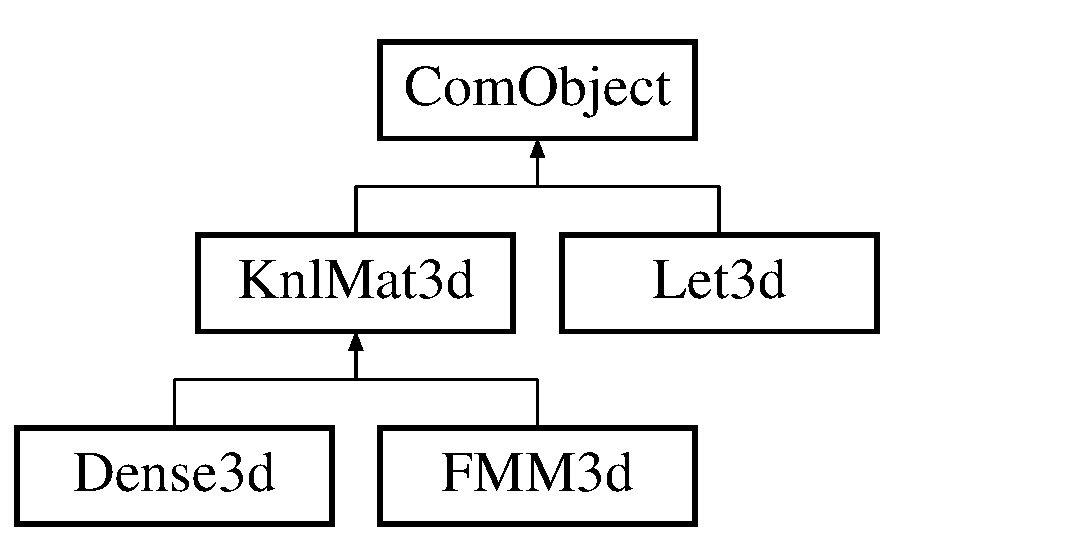
\includegraphics[height=3cm]{classComObject}
\end{center}
\end{figure}


\subsection{Detailed Description}
Com\-Object class for communication purposes. For sequential code, Com\-Object does very little. See comobject\_\-mpi.hpp for parallel code and how it is used $\ast$/. 



Definition at line 27 of file comobject.hpp.\subsection*{Public Member Functions}
\begin{CompactItemize}
\item 
{\bf Com\-Object} (const string \&prefix)
\item 
virtual {\bf $\sim$Com\-Object} ()
\item 
const string \& {\bf prefix} ()
\end{CompactItemize}
\subsection*{Protected Attributes}
\begin{CompactItemize}
\item 
string {\bf \_\-prefix}
\end{CompactItemize}


\subsection{Constructor \& Destructor Documentation}
\index{ComObject@{Com\-Object}!ComObject@{ComObject}}
\index{ComObject@{ComObject}!ComObject@{Com\-Object}}
\subsubsection{\setlength{\rightskip}{0pt plus 5cm}Com\-Object::Com\-Object (const string \& {\em prefix})\hspace{0.3cm}{\tt  [inline]}}\label{classComObject_cf233a08894f1cdd0f9bfb83b3251686_cf233a08894f1cdd0f9bfb83b3251686}


Initialize Com\-Object using string prefix 

Definition at line 34 of file comobject.hpp.

\footnotesize\begin{verbatim}34 : _prefix(prefix) {;}
\end{verbatim}\normalsize 


\index{ComObject@{Com\-Object}!~ComObject@{$\sim$ComObject}}
\index{~ComObject@{$\sim$ComObject}!ComObject@{Com\-Object}}
\subsubsection{\setlength{\rightskip}{0pt plus 5cm}virtual Com\-Object::$\sim$Com\-Object ()\hspace{0.3cm}{\tt  [inline, virtual]}}\label{classComObject_cf63f06cbc455a408453fe3d9d3dea0a_cf63f06cbc455a408453fe3d9d3dea0a}


Destroy Com\-Object 

Definition at line 36 of file comobject.hpp.

\footnotesize\begin{verbatim}36 {;}
\end{verbatim}\normalsize 




\subsection{Member Function Documentation}
\index{ComObject@{Com\-Object}!prefix@{prefix}}
\index{prefix@{prefix}!ComObject@{Com\-Object}}
\subsubsection{\setlength{\rightskip}{0pt plus 5cm}const string\& Com\-Object::prefix ()\hspace{0.3cm}{\tt  [inline]}}\label{classComObject_8171d0694121d77c4bfba18e5745faa9_8171d0694121d77c4bfba18e5745faa9}


Return \_\-prefic string 

Definition at line 39 of file comobject.hpp.

References \_\-prefix.

Referenced by Let3d::setup(), and FMM3d::setup().

\footnotesize\begin{verbatim}39 { return _prefix; }  
\end{verbatim}\normalsize 




\subsection{Member Data Documentation}
\index{ComObject@{Com\-Object}!_prefix@{\_\-prefix}}
\index{_prefix@{\_\-prefix}!ComObject@{Com\-Object}}
\subsubsection{\setlength{\rightskip}{0pt plus 5cm}string {\bf Com\-Object::\_\-prefix}\hspace{0.3cm}{\tt  [protected]}}\label{classComObject_b933f996cea3f524cf1514eb8539edfa_b933f996cea3f524cf1514eb8539edfa}


\_\-prefix is a string such as \char`\"{}fmm3d\_\-\char`\"{} which describes the type of object this is 

Definition at line 31 of file comobject.hpp.

Referenced by prefix().

The documentation for this class was generated from the following file:\begin{CompactItemize}
\item 
fmm3d/{\bf comobject.hpp}\end{CompactItemize}

\section{Dense3d Class Reference}
\label{classDense3d}\index{Dense3d@{Dense3d}}
{\tt \#include $<$dense3d.hpp$>$}

Inheritance diagram for Dense3d::\begin{figure}[H]
\begin{center}
\leavevmode
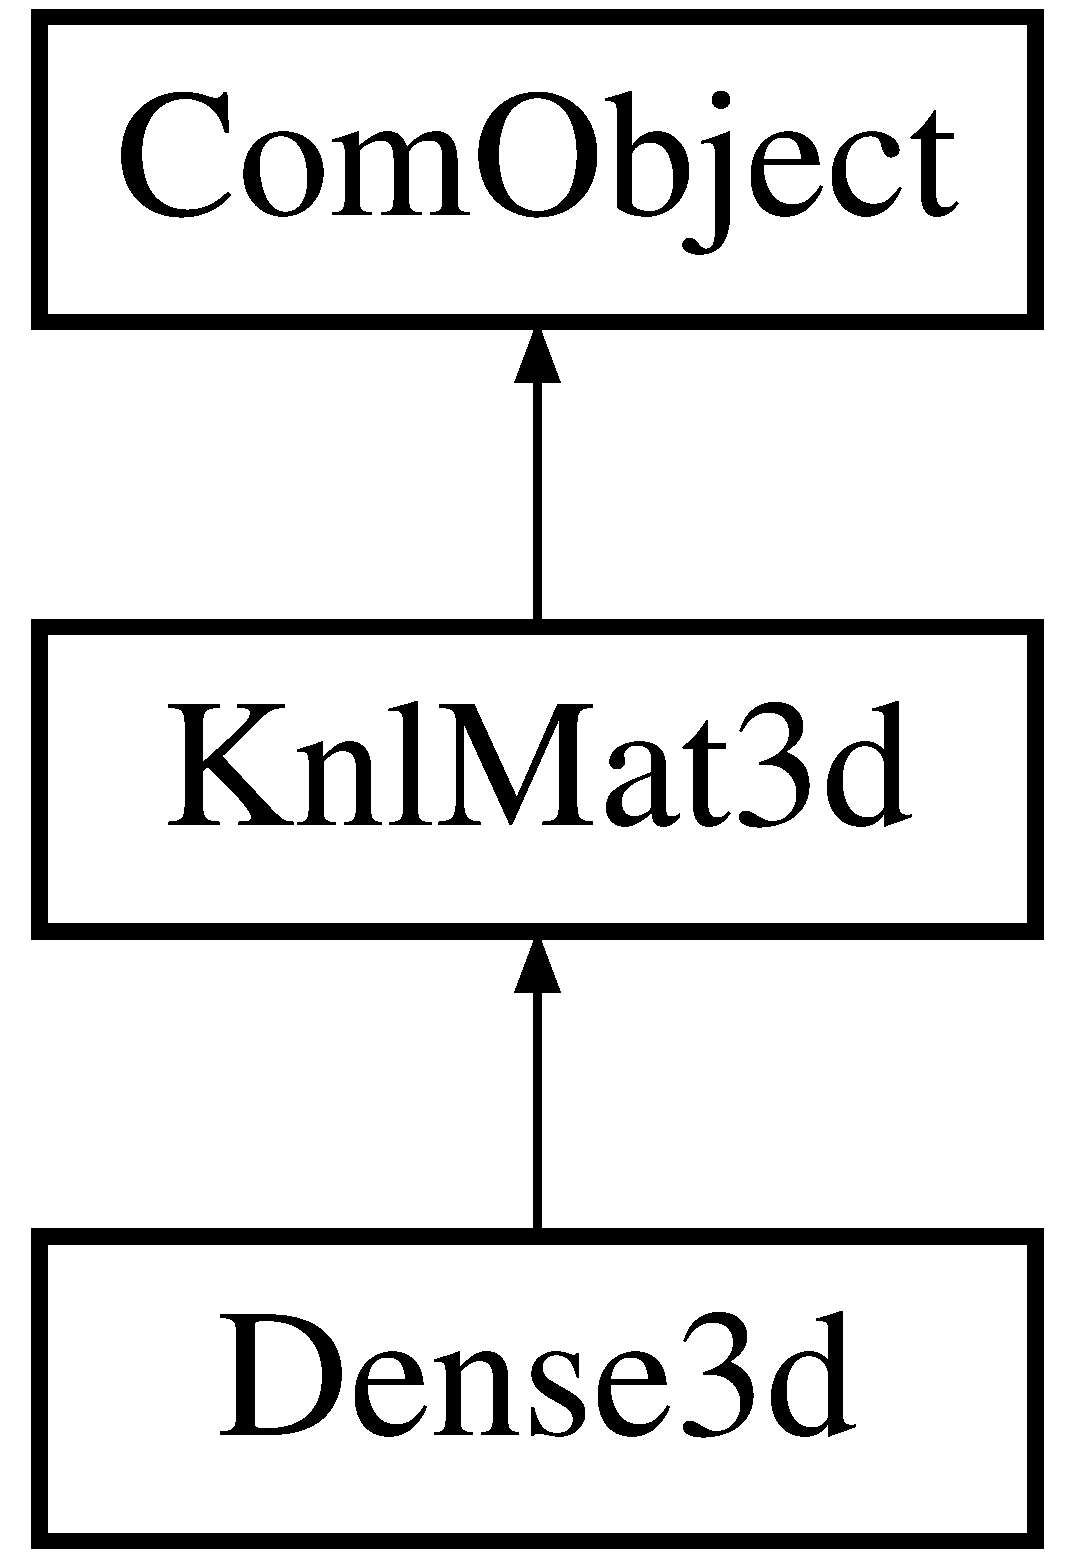
\includegraphics[height=3cm]{classDense3d}
\end{center}
\end{figure}


\subsection{Detailed Description}
Dense3d implements the virtual setup and eval functions of {\bf Knl\-Mat3d}{\rm (p.\,\pageref{classKnlMat3d})} $\ast$/. 



Definition at line 26 of file dense3d.hpp.\subsection*{Public Member Functions}
\begin{CompactItemize}
\item 
{\bf Dense3d} (const string \&p)
\item 
{\bf $\sim$Dense3d} ()
\item 
int {\bf setup} (map$<$ string, string $>$ \&)
\item 
int {\bf evaluate} (const Dbl\-Num\-Vec \&src\-Den, Dbl\-Num\-Vec \&trg\-Val)
\end{CompactItemize}


\subsection{Constructor \& Destructor Documentation}
\index{Dense3d@{Dense3d}!Dense3d@{Dense3d}}
\index{Dense3d@{Dense3d}!Dense3d@{Dense3d}}
\subsubsection{\setlength{\rightskip}{0pt plus 5cm}Dense3d::Dense3d (const string \& {\em p})}\label{classDense3d_26942f58b7764c78dc6281f8bf79c4b5_26942f58b7764c78dc6281f8bf79c4b5}


Dense3d constructor takes string to declare type 

Definition at line 22 of file dense3d.cpp.

\footnotesize\begin{verbatim}22                                : KnlMat3d(p)
23 {
24 }
\end{verbatim}\normalsize 


\index{Dense3d@{Dense3d}!~Dense3d@{$\sim$Dense3d}}
\index{~Dense3d@{$\sim$Dense3d}!Dense3d@{Dense3d}}
\subsubsection{\setlength{\rightskip}{0pt plus 5cm}Dense3d::$\sim$Dense3d ()}\label{classDense3d_465b01ffd81006def662ecab05e22099_465b01ffd81006def662ecab05e22099}


Dense3d destructor 

Definition at line 26 of file dense3d.cpp.

\footnotesize\begin{verbatim}27 {
28 }
\end{verbatim}\normalsize 




\subsection{Member Function Documentation}
\index{Dense3d@{Dense3d}!evaluate@{evaluate}}
\index{evaluate@{evaluate}!Dense3d@{Dense3d}}
\subsubsection{\setlength{\rightskip}{0pt plus 5cm}int Dense3d::evaluate (const Dbl\-Num\-Vec \& {\em src\-Den}, Dbl\-Num\-Vec \& {\em trg\-Val})\hspace{0.3cm}{\tt  [virtual]}}\label{classDense3d_3d2ce8cfb3d9632d6b69352f1bb5eda2_3d2ce8cfb3d9632d6b69352f1bb5eda2}


Virtual evaluation function 

Implements {\bf Knl\-Mat3d} {\rm (p.\,\pageref{classKnlMat3d_fcf3de1e6ce4ee024ef0d320363bd920_fcf3de1e6ce4ee024ef0d320363bd920})}.

Definition at line 39 of file dense3d.cpp.

References Knl\-Mat3d::\_\-knl, Knl\-Mat3d::\_\-src\-Nor, Knl\-Mat3d::\_\-src\-Pos, Knl\-Mat3d::dim(), Kernel3d::kernel(), Knl\-Mat3d::src\-DOF(), and Knl\-Mat3d::trg\-DOF().

\footnotesize\begin{verbatim}40 {
41   //-----------------------------------
42   iA(srcDen.m()==srcDOF()*(*_srcPos).n());  iA(trgVal.m()==trgDOF()*(*_trgPos).n());
43   
44   int dim  = this->dim();
45   int srcDOF = this->srcDOF();
46   int trgDOF = this->trgDOF();
47   /* Number of sources */
48   int numSrc = (*_srcPos).n();
49   /* Number of targets */
50   int numTrg = (*_trgPos).n();
51   
52   DblNumMat inter(trgDOF, numSrc*srcDOF);
53   for(int i=0; i<numTrg; i++) {
54          DblNumMat onePosMat(dim, 1, false, (*_trgPos).clmdata(i));
55          DblNumVec oneValVec(trgDOF, false, trgVal.data()+trgDOF*i);
56          iC( _knl.kernel((*_srcPos), (*_srcNor), onePosMat, inter) );
57          iC( dgemv(1.0, inter, srcDen, 0.0, oneValVec) );
58   }
59   
60   return 0;
61 }
\end{verbatim}\normalsize 


\index{Dense3d@{Dense3d}!setup@{setup}}
\index{setup@{setup}!Dense3d@{Dense3d}}
\subsubsection{\setlength{\rightskip}{0pt plus 5cm}int Dense3d::setup (map$<$ string, string $>$ \&)\hspace{0.3cm}{\tt  [virtual]}}\label{classDense3d_6c9d66eef2ad01ccfea65cb116bf5726_6c9d66eef2ad01ccfea65cb116bf5726}


Virtual setup function 

Implements {\bf Knl\-Mat3d} {\rm (p.\,\pageref{classKnlMat3d_24cbbecf677cd909a522d252feebf2c6_24cbbecf677cd909a522d252feebf2c6})}.

Definition at line 31 of file dense3d.cpp.

References Knl\-Mat3d::\_\-src\-Nor, Knl\-Mat3d::\_\-src\-Pos, Knl\-Mat3d::\_\-trg\-Pos, and Knl\-Mat3d::dim().

\footnotesize\begin{verbatim}32 {
33   iA(_srcPos!=NULL && _srcNor!=NULL && _trgPos!=NULL);
34   iA((*_srcPos).m()==dim() && (*_trgPos).m()==dim());  //nothing to do
35   return 0;
36 }
\end{verbatim}\normalsize 




The documentation for this class was generated from the following files:\begin{CompactItemize}
\item 
fmm3d/{\bf dense3d.hpp}\item 
fmm3d/{\bf dense3d.cpp}\end{CompactItemize}

\section{FMM3d Class Reference}
\label{classFMM3d}\index{FMM3d@{FMM3d}}
{\tt \#include $<$fmm3d.hpp$>$}

Inheritance diagram for FMM3d::\begin{figure}[H]
\begin{center}
\leavevmode
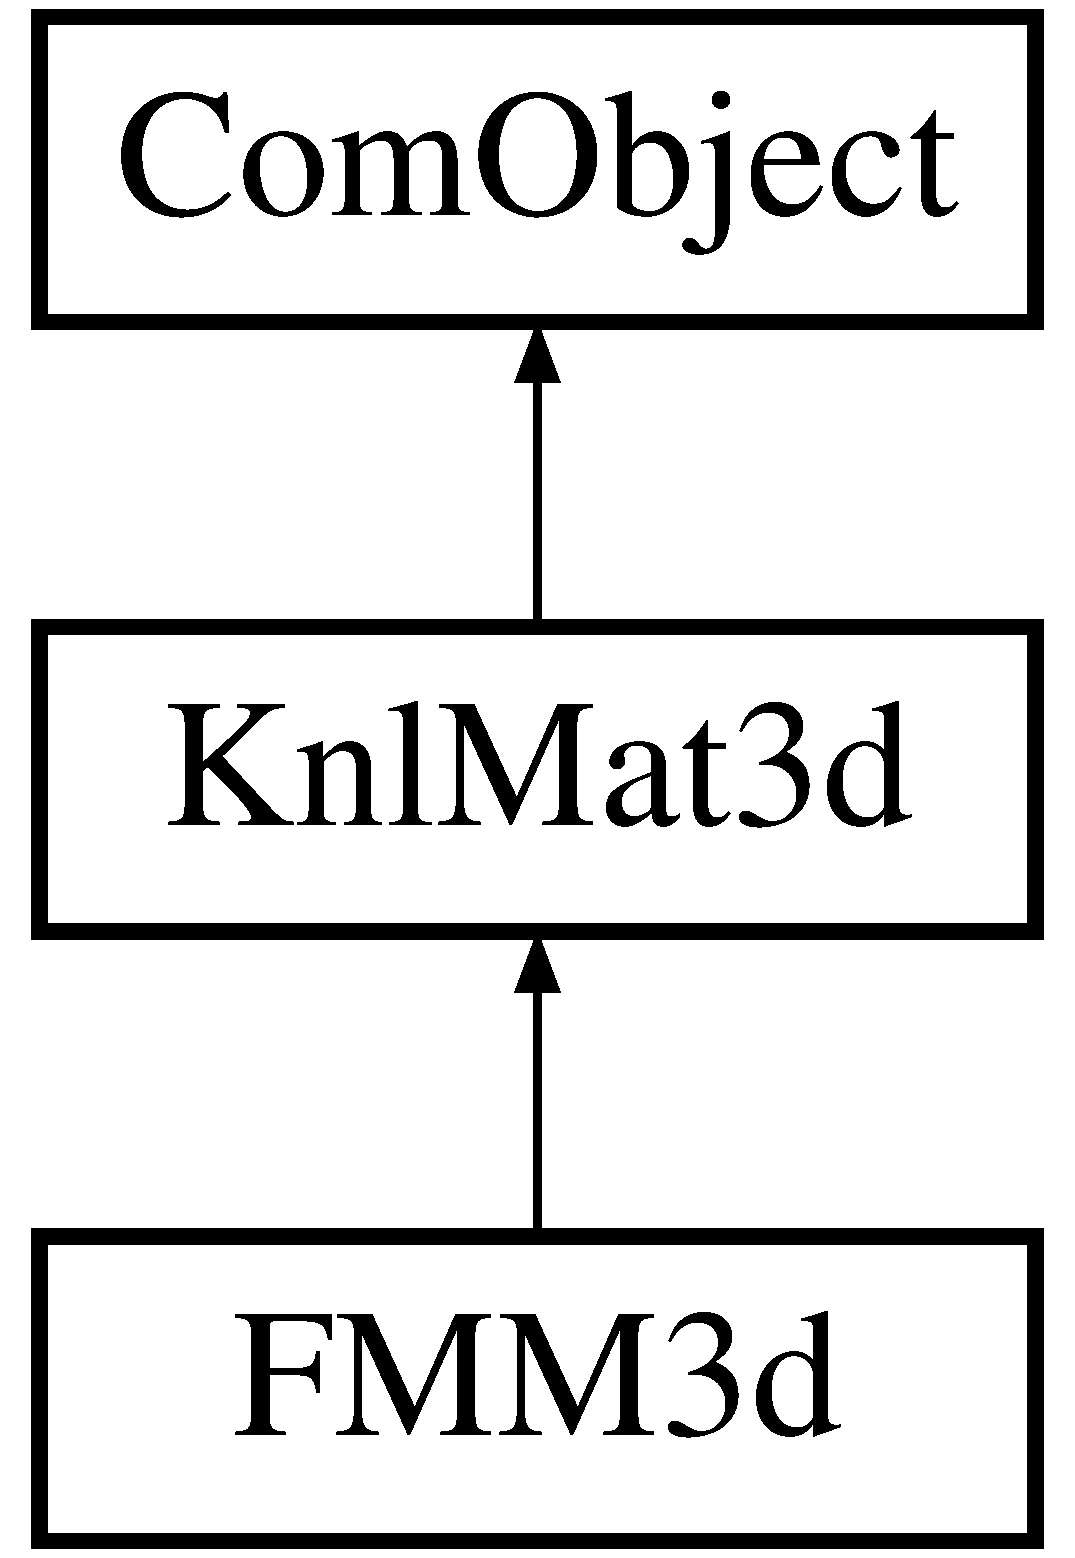
\includegraphics[height=3cm]{classFMM3d}
\end{center}
\end{figure}


\subsection{Detailed Description}
FMM3d sequential class. 

FMM3d implements {\bf Knl\-Mat3d}{\rm (p.\,\pageref{classKnlMat3d})} 



Definition at line 31 of file fmm3d.hpp.\subsection*{Public Types}
\begin{CompactItemize}
\item 
typedef pair$<$ int, int $>$ {\bf intpair}
\item 
enum \{ {\bf UE} = 0, 
{\bf UC} = 1, 
{\bf DE} = 2, 
{\bf DC} = 3
 \}
\end{CompactItemize}
\subsection*{Public Member Functions}
\begin{CompactItemize}
\item 
{\bf FMM3d} (const string \&p)
\item 
{\bf $\sim$FMM3d} ()
\item 
Point3 \& {\bf center} ()
\item 
int \& {\bf root\-Level} ()
\item 
int \& {\bf np} ()
\item 
int {\bf setup} (map$<$ string, string $>$ \&opts)
\item 
int {\bf evaluate} (const Dbl\-Num\-Vec \&src\-Den, Dbl\-Num\-Vec \&trg\-Val)
\item 
int {\bf check} (const Dbl\-Num\-Vec \&src\-Den, Dbl\-Num\-Vec \&trg\-Val, int num\-Chk, double \&relative\-Err)
\item 
{\bf Let3d} $\ast$ {\bf let} ()
\item 
{\bf Mat\-Mgnt3d} $\ast$ {\bf matmgnt} ()
\item 
vector$<$ {\bf Node} $>$ \& {\bf node\-Vec} ()
\item 
{\bf Node} \& {\bf node} (int g\-Node\-Idx)
\end{CompactItemize}
\subsection*{Protected Member Functions}
\begin{CompactItemize}
\item 
int {\bf dat\-Sze} (int tp)
\item 
int {\bf Src\-Equ2Trg\-Chk\_\-dgemv} (const Dbl\-Num\-Mat \&src\-Pos, const Dbl\-Num\-Mat \&src\-Nor, const Dbl\-Num\-Mat \&trg\-Pos, const Dbl\-Num\-Vec \&src\-Den, Dbl\-Num\-Vec \&trg\-Val)
\item 
int {\bf Src\-Equ2Upw\-Chk\_\-dgemv} (const Dbl\-Num\-Mat \&src\-Pos, const Dbl\-Num\-Mat \&src\-Nor, Point3 trg\-Ctr, double trg\-Rad, const Dbl\-Num\-Vec \&src\-Den, Dbl\-Num\-Vec \&trg\-Val)
\item 
int {\bf Src\-Equ2Dwn\-Chk\_\-dgemv} (const Dbl\-Num\-Mat \&src\-Pos, const Dbl\-Num\-Mat \&src\-Nor, Point3 trg\-Ctr, double trg\-Rad, const Dbl\-Num\-Vec \&src\-Den, Dbl\-Num\-Vec \&trg\-Val)
\item 
int {\bf Dwn\-Equ2Trg\-Chk\_\-dgemv} (Point3 src\-Ctr, double src\-Rad, const Dbl\-Num\-Mat \&trg\-Pos, const Dbl\-Num\-Vec \&src\-Den, Dbl\-Num\-Vec \&trg\-Val)
\item 
int {\bf Upw\-Equ2Trg\-Chk\_\-dgemv} (Point3 src\-Ctr, double src\-Rad, const Dbl\-Num\-Mat \&trg\-Pos, const Dbl\-Num\-Vec \&src\-Den, Dbl\-Num\-Vec \&trg\-Val)
\item 
Dbl\-Num\-Mat {\bf src\-Exa\-Pos} (int g\-Node\-Idx)
\item 
Dbl\-Num\-Mat {\bf src\-Exa\-Nor} (int g\-Node\-Idx)
\item 
Dbl\-Num\-Vec {\bf src\-Exa\-Den} (int g\-Node\-Idx)
\item 
Dbl\-Num\-Vec {\bf src\-Upw\-Equ\-Den} (int g\-Node\-Idx)
\item 
Dbl\-Num\-Vec {\bf src\-Upw\-Chk\-Val} (int g\-Node\-Idx)
\item 
Dbl\-Num\-Mat {\bf trg\-Exa\-Pos} (int g\-Node\-Idx)
\item 
Dbl\-Num\-Vec {\bf trg\-Exa\-Val} (int g\-Node\-Idx)
\item 
Dbl\-Num\-Vec {\bf trg\-Dwn\-Equ\-Den} (int g\-Node\-Idx)
\item 
Dbl\-Num\-Vec {\bf trg\-Dwn\-Chk\-Val} (int g\-Node\-Idx)
\item 
int {\bf src\-Data} ()
\item 
int {\bf trg\-Data} ()
\end{CompactItemize}
\subsection*{Protected Attributes}
\begin{CompactItemize}
\item 
Point3 {\bf \_\-center}
\item 
int {\bf \_\-root\-Level}
\item 
int {\bf \_\-np}
\item 
{\bf Let3d} $\ast$ {\bf \_\-let}
\item 
{\bf Mat\-Mgnt3d} $\ast$ {\bf \_\-matmgnt}
\item 
vector$<$ {\bf Node} $>$ {\bf \_\-node\-Vec}
\item 
Dbl\-Num\-Mat {\bf \_\-src\-Exa\-Pos}
\item 
Dbl\-Num\-Mat {\bf \_\-src\-Exa\-Nor}
\item 
Dbl\-Num\-Vec {\bf \_\-src\-Exa\-Den}
\item 
Dbl\-Num\-Vec {\bf \_\-src\-Upw\-Equ\-Den}
\item 
Dbl\-Num\-Vec {\bf \_\-src\-Upw\-Chk\-Val}
\item 
Dbl\-Num\-Mat {\bf \_\-trg\-Exa\-Pos}
\item 
Dbl\-Num\-Vec {\bf \_\-trg\-Exa\-Val}
\item 
Dbl\-Num\-Vec {\bf \_\-trg\-Dwn\-Equ\-Den}
\item 
Dbl\-Num\-Vec {\bf \_\-trg\-Dwn\-Chk\-Val}
\item 
{\bf Kernel3d} {\bf \_\-knl\_\-mm}
\item 
int {\bf \_\-mul\_\-mm}
\end{CompactItemize}
\subsection*{Classes}
\begin{CompactItemize}
\item 
class {\bf Node}
\begin{CompactList}\small\item\em {\bf Node}{\rm (p.\,\pageref{classFMM3d_1_1Node})} Class for {\bf FMM3d}{\rm (p.\,\pageref{classFMM3d})}. \item\end{CompactList}\end{CompactItemize}


\subsection{Member Typedef Documentation}
\index{FMM3d@{FMM3d}!intpair@{intpair}}
\index{intpair@{intpair}!FMM3d@{FMM3d}}
\subsubsection{\setlength{\rightskip}{0pt plus 5cm}typedef pair$<$int,int$>$ {\bf FMM3d::intpair}}\label{classFMM3d_516fcca2e14cd2e14fd71db54824f696_516fcca2e14cd2e14fd71db54824f696}




Definition at line 34 of file fmm3d.hpp.

\subsection{Member Enumeration Documentation}
\subsubsection{\setlength{\rightskip}{0pt plus 5cm}anonymous enum}\label{classFMM3d_dca29a1140aadadfd92b34a02fa516ef_dca29a1140aadadfd92b34a02fa516ef}


UE = Upper Equivalent UC = Upper Check DE = Downward Equivalent DC = Downward Check \begin{Desc}
\item[Enumerator: ]\par
\begin{description}
\index{UE@{UE}!FMM3d@{FMM3d}}\index{FMM3d@{FMM3d}!UE@{UE}}\item[{\em 
UE\label{classFMM3d_dca29a1140aadadfd92b34a02fa516ef_dca29a1140aadadfd92b34a02fa516ef0612e93d65abcdaeed533a0876474251}
}]\index{UC@{UC}!FMM3d@{FMM3d}}\index{FMM3d@{FMM3d}!UC@{UC}}\item[{\em 
UC\label{classFMM3d_dca29a1140aadadfd92b34a02fa516ef_dca29a1140aadadfd92b34a02fa516ef6a2fb30a2dacdda4d74122697262a8b7}
}]\index{DE@{DE}!FMM3d@{FMM3d}}\index{FMM3d@{FMM3d}!DE@{DE}}\item[{\em 
DE\label{classFMM3d_dca29a1140aadadfd92b34a02fa516ef_dca29a1140aadadfd92b34a02fa516ef3a52f3c22ed6fcde5bf696a6c02c9e73}
}]\index{DC@{DC}!FMM3d@{FMM3d}}\index{FMM3d@{FMM3d}!DC@{DC}}\item[{\em 
DC\label{classFMM3d_dca29a1140aadadfd92b34a02fa516ef_dca29a1140aadadfd92b34a02fa516efcf75e54791dd1f49f918345fdfe2430b}
}]\end{description}
\end{Desc}



Definition at line 40 of file fmm3d.hpp.

\footnotesize\begin{verbatim}40 {        UE=0,   UC=1,   DE=2,   DC=3,  };
\end{verbatim}\normalsize 




\subsection{Constructor \& Destructor Documentation}
\index{FMM3d@{FMM3d}!FMM3d@{FMM3d}}
\index{FMM3d@{FMM3d}!FMM3d@{FMM3d}}
\subsubsection{\setlength{\rightskip}{0pt plus 5cm}FMM3d::FMM3d (const string \& {\em p})}\label{classFMM3d_c6779767af55d215c788dcaf4dfbaf6e_c6779767af55d215c788dcaf4dfbaf6e}




Definition at line 23 of file fmm3d.cpp.

\footnotesize\begin{verbatim}23                            :
24   KnlMat3d(p), _center(0,0,0), _rootLevel(0),
25   _np(6), _let(NULL), _matmgnt(NULL)
26 {
27 }

\end{verbatim}\normalsize 


\index{FMM3d@{FMM3d}!~FMM3d@{$\sim$FMM3d}}
\index{~FMM3d@{$\sim$FMM3d}!FMM3d@{FMM3d}}
\subsubsection{\setlength{\rightskip}{0pt plus 5cm}FMM3d::$\sim$FMM3d ()}\label{classFMM3d_95ad154aae7c25cde0cc2a7108470c36_95ad154aae7c25cde0cc2a7108470c36}




Definition at line 29 of file fmm3d.cpp.

References \_\-let.

\footnotesize\begin{verbatim}30 {
31   if(_let!=NULL)         delete _let;
32 }
\end{verbatim}\normalsize 




\subsection{Member Function Documentation}
\index{FMM3d@{FMM3d}!center@{center}}
\index{center@{center}!FMM3d@{FMM3d}}
\subsubsection{\setlength{\rightskip}{0pt plus 5cm}Point3\& FMM3d::center ()\hspace{0.3cm}{\tt  [inline]}}\label{classFMM3d_5c0517b22b09f08712cbfd01aa1f29d7_5c0517b22b09f08712cbfd01aa1f29d7}


Return center of toplevel box 

Definition at line 109 of file fmm3d.hpp.

References \_\-center.

\footnotesize\begin{verbatim}109 { return _center; }
\end{verbatim}\normalsize 


\index{FMM3d@{FMM3d}!check@{check}}
\index{check@{check}!FMM3d@{FMM3d}}
\subsubsection{\setlength{\rightskip}{0pt plus 5cm}int FMM3d::check (const Dbl\-Num\-Vec \& {\em src\-Den}, Dbl\-Num\-Vec \& {\em trg\-Val}, int {\em num\-Chk}, double \& {\em relative\-Err})}\label{classFMM3d_03ae26a8343213f8e305ed8df685173f_03ae26a8343213f8e305ed8df685173f}


Check relative error - in fmm\_\-check.cpp 

Definition at line 25 of file fmm3d\_\-check.cpp.

References Knl\-Mat3d::\_\-src\-Pos, Knl\-Mat3d::\_\-trg\-Pos, Knl\-Mat3d::dim(), Knl\-Mat3d::src\-DOF(), and Knl\-Mat3d::trg\-DOF().

\footnotesize\begin{verbatim}26 {
27   iA(_trgPos->n()>0); //have things to check
28   int dim = this->dim();
29   int srcDOF = this->srcDOF();
30   int trgDOF = this->trgDOF();
31   int srcNum = _srcPos->n();
32   int trgNum = _trgPos->n();   //int lclnum = this->lclnum();
33   
34   //1. select point to check
35   vector<int> chkVec(numChk);
36   for(int k=0; k<numChk; k++) {
37          chkVec[k] = int( floor(drand48()*trgNum) );     iA(chkVec[k]>=0 && chkVec[k]<trgNum);
38   }
39   DblNumMat ChkPos(dim, numChk);
40   DblNumVec chkVal(numChk*trgDOF);
41   DblNumVec chkDen(numChk*trgDOF);
42   for(int k=0; k<numChk; k++) {
43          for(int i=0; i<dim; i++)               ChkPos(i, k) = (*_trgPos)(i, chkVec[k]);
44          for(int i=0; i<trgDOF;i++)             chkVal(k*trgDOF+i) = trgVal(chkVec[k]*trgDOF+i);
45   }
46   
47   //2. compute and gather
48   DblNumMat inter(trgDOF, srcNum*srcDOF);
49   for(int i=0; i<numChk; i++) {
50          DblNumMat oneChkPos(dim, 1, false, ChkPos.clmdata(i));
51          DblNumVec onechkDen(trgDOF, false, chkDen.data()+i*trgDOF);
52          iC( _knl.kernel(*_srcPos, *_srcNor, oneChkPos, inter) );
53          iC( dgemv(1.0, inter, srcden, 0.0, onechkDen) );
54   }
55   
56   //3. distribute to individual
57   for(int k=0; k<numChk; k++)
58          for(int i=0; i<trgDOF; i++)
59                 chkDen(k*trgDOF+i) -= chkVal(k*trgDOF+i);
60   
61   double vn = 0;  double en = 0;
62   for(int k=0; k<numChk; k++)
63          for(int i=0; i<trgDOF; i++) {
64                 vn += chkVal(k*trgDOF+i) * chkVal(k*trgDOF+i);
65                 en += chkDen(k*trgDOF+i) * chkDen(k*trgDOF+i);
66          }
67   vn = sqrt(vn);
68   en = sqrt(en);
69   
70   //cerr<<"relative error: "<<en/vn<<endl;  cerr<<"error norm    : "<<en<<endl;  cerr<<"solution norm : "<<vn<<endl;
71   rerr = en/vn; //relative error
72   
73   return 0;
74 }
\end{verbatim}\normalsize 


\index{FMM3d@{FMM3d}!datSze@{datSze}}
\index{datSze@{datSze}!FMM3d@{FMM3d}}
\subsubsection{\setlength{\rightskip}{0pt plus 5cm}int FMM3d::dat\-Sze (int {\em tp})\hspace{0.3cm}{\tt  [inline, protected]}}\label{classFMM3d_e698f5e6e784c12d19a62b0d40456fc6_e698f5e6e784c12d19a62b0d40456fc6}


Data Size 

Definition at line 128 of file fmm3d.hpp.

References \_\-matmgnt, and Mat\-Mgnt3d::pln\-Dat\-Sze().

Referenced by src\-Data(), src\-Upw\-Chk\-Val(), src\-Upw\-Equ\-Den(), trg\-Data(), trg\-Dwn\-Chk\-Val(), and trg\-Dwn\-Equ\-Den().

\footnotesize\begin{verbatim}128 { return _matmgnt->plnDatSze(tp); }
\end{verbatim}\normalsize 


\index{FMM3d@{FMM3d}!DwnEqu2TrgChk_dgemv@{DwnEqu2TrgChk\_\-dgemv}}
\index{DwnEqu2TrgChk_dgemv@{DwnEqu2TrgChk\_\-dgemv}!FMM3d@{FMM3d}}
\subsubsection{\setlength{\rightskip}{0pt plus 5cm}int FMM3d::Dwn\-Equ2Trg\-Chk\_\-dgemv (Point3 {\em src\-Ctr}, double {\em src\-Rad}, const Dbl\-Num\-Mat \& {\em trg\-Pos}, const Dbl\-Num\-Vec \& {\em src\-Den}, Dbl\-Num\-Vec \& {\em trg\-Val})\hspace{0.3cm}{\tt  [protected]}}\label{classFMM3d_044a9a8966c365ba77585ecc38a2073e_044a9a8966c365ba77585ecc38a2073e}


Downward Equivalent To Target Check 

Definition at line 84 of file fmm3d.cpp.

References \_\-knl\_\-mm, \_\-matmgnt, DE, Kernel3d::kernel(), Mat\-Mgnt3d::local\-Pos(), Kernel3d::src\-DOF(), and Kernel3d::trg\-DOF().

\footnotesize\begin{verbatim}85 {
86   int TMAX = 1024;
87   if(trgPos.n()<=TMAX) {
88          DblNumMat srcPos; iC( _matmgnt->localPos(DE, srcCtr, srcRad, srcPos) );
89          int M = trgPos.n() * _knl_mm.trgDOF();
90          int N = srcPos.n() * _knl_mm.srcDOF();
91          DblNumMat tmp(M,N);
92          iC( _knl_mm.kernel(srcPos, srcPos, trgPos, tmp) );
93          iC( dgemv(1.0, tmp, srcDen, 1.0, trgVal) );
94   } else {
95          DblNumMat srcPos; iC( _matmgnt->localPos(DE, srcCtr, srcRad, srcPos) );
96          int RUNS = (trgPos.n()-1) / TMAX + 1;
97          for(int r=0; r<RUNS; r++) {
98                 int stt = r*TMAX;
99                 int end = min((r+1)*TMAX, trgPos.n());
100                 int num = end-stt;
101                 int M = num * _knl_mm.trgDOF();
102                 int N = srcPos.n() * _knl_mm.srcDOF();
103                 DblNumMat tps(dim(), num, false, trgPos.data() + stt*dim());
104                 DblNumVec tvl(num*_knl_mm.trgDOF(), false, trgVal.data() + stt*_knl_mm.trgDOF());
105                 DblNumMat tmp(M, N);
106                 iC( _knl_mm.kernel(srcPos, srcPos, tps, tmp) );
107                 iC( dgemv(1.0, tmp, srcDen, 1.0, tvl) );
108          }
109   }
110   return 0;
111 }
\end{verbatim}\normalsize 


\index{FMM3d@{FMM3d}!evaluate@{evaluate}}
\index{evaluate@{evaluate}!FMM3d@{FMM3d}}
\subsubsection{\setlength{\rightskip}{0pt plus 5cm}int FMM3d::evaluate (const Dbl\-Num\-Vec \& {\em src\-Den}, Dbl\-Num\-Vec \& {\em trg\-Val})\hspace{0.3cm}{\tt  [virtual]}}\label{classFMM3d_3d2ce8cfb3d9632d6b69352f1bb5eda2_3d2ce8cfb3d9632d6b69352f1bb5eda2}


Evaluate - in {\bf fmm3d\_\-eval.cpp}{\rm (p.\,\pageref{fmm3d__eval_8cpp})} 

Implements {\bf Knl\-Mat3d} {\rm (p.\,\pageref{classKnlMat3d_fcf3de1e6ce4ee024ef0d320363bd920_fcf3de1e6ce4ee024ef0d320363bd920})}.

Definition at line 25 of file fmm3d\_\-eval.cpp.

References \_\-let, \_\-matmgnt, \_\-src\-Exa\-Den, \_\-src\-Upw\-Chk\-Val, \_\-src\-Upw\-Equ\-Den, \_\-trg\-Dwn\-Chk\-Val, \_\-trg\-Dwn\-Equ\-Den, \_\-trg\-Exa\-Val, LET\_\-SRCNODE, Let3d::node(), Mat\-Mgnt3d::report(), Knl\-Mat3d::src\-DOF(), src\-Exa\-Den(), Let3d::tag(), Let3d::terminal(), Knl\-Mat3d::trg\-DOF(), and Let3d::upw\-Order\-Collect().

\footnotesize\begin{verbatim}26 {
27   _matmgnt->report();
28   //-----------------------------------
29   iA(srcDen.m()==srcDOF()*(*_srcPos).n());  iA(trgVal.m()==trgDOF()*(*_trgPos).n());
30   
31   //cerr<<"fmm src and trg numbers "<<pglbnum(_srcPos)<<" "<<pglbnum(_trgPos)<<endl;
32   int srcDOF = this->srcDOF();
33   int trgDOF = this->trgDOF();
34   
35   //1. zero out Vecs
36   setvalue(trgVal, 0.0);
37   
38   setvalue(_srcExaDen, 0.0);
39   setvalue(_srcUpwEquDen, 0.0);
40   setvalue(_srcUpwChkVal, 0.0);
41   
42   setvalue(_trgExaVal, 0.0);
43   setvalue(_trgDwnEquDen, 0.0);
44   setvalue(_trgDwnChkVal, 0.0);
45   clock_t ck0, ck1;
46   //CLOCKING;
47   ck0 = clock();
48   vector<int> ordVec; iC( _let->upwOrderCollect(ordVec) ); //BOTTOM UP
49 
50   //2. for cbtr, load ExaDen
51   ck0 = clock();
52   for(int i=0; i<ordVec.size(); i++) {
53          int gNodeIdx = ordVec[i];
54          if(_let->tag(gNodeIdx) & LET_SRCNODE) {
55                 if(_let->terminal(gNodeIdx)==true) {
56                   DblNumVec srcExaDen(this->srcExaDen(gNodeIdx));
57                   vector<int>& curVecIdxs = _let->node(gNodeIdx).srcOwnVecIdxs();
58                   for(int k=0; k<curVecIdxs.size(); k++) {
59                          int poff = curVecIdxs[k];
60                          for(int d=0; d<srcDOF; d++) {
61                                 srcExaDen(k*srcDOF+d) = srcDen(poff*srcDOF+d);
62                          }
63                   }
64                 }
65          }
66   }
67   //ck1 = clock();  cerr<<"load  "<<double(ck1-ck0)/CLOCKS_PER_SEC<<endl;  
68   
69   //3. up computation
70   ck0 = clock();
71   for(int i=0; i<ordVec.size(); i++) {
72          int gNodeIdx = ordVec[i];
73          if(_let->tag(gNodeIdx) & LET_SRCNODE) {                //GNTra gnt = _let->gNodeIdx2gnt(gNodeIdx);
74                 //if(_let->depth(gNodeIdx)>=2) {
75                 if(_let->depth(gNodeIdx)>=0) {
76                   DblNumVec srcUpwChkValgNodeIdx(srcUpwChkVal(gNodeIdx));
77                   DblNumVec srcUpwEquDengNodeIdx(srcUpwEquDen(gNodeIdx));
78                   if(_let->terminal(gNodeIdx)==true) {
79                          //S2M - Source -> Multipole Exapnsion
80                          iC( SrcEqu2UpwChk_dgemv(srcExaPos(gNodeIdx), srcExaNor(gNodeIdx), _let->center(gNodeIdx), _let->radius(gNodeIdx), srcExaDen(gNodeIdx), srcUpwChkValgNodeIdx) );
81                   } else {
82                          //M2M - Multipole -> Multipole
83                          for(int a=0; a<2; a++) {
84                                 for(int b=0; b<2; b++) {
85                                   for(int c=0; c<2; c++) {
86                                          Index3 idx(a,b,c);
87                                          int chi = _let->child(gNodeIdx, idx);
88                                          if(_let->tag(chi) & LET_SRCNODE) {
89                                                 iC( _matmgnt->UpwEqu2UpwChk_dgemv(_let->depth(chi)+_rootLevel, idx, srcUpwEquDen(chi), srcUpwChkValgNodeIdx) );
90                                          }
91                                   }
92                                 }
93                          }
94                   }
95                   //M2M - Multipole -> Multipole
96                   iC( _matmgnt->UpwChk2UpwEqu_dgemv(_let->depth(gNodeIdx)+_rootLevel, srcUpwChkValgNodeIdx, srcUpwEquDengNodeIdx) );
97                 }
98          }
99   }
100   ordVec.clear();  iC( _let->dwnOrderCollect(ordVec) );
101   //U - list contribution calculation
102   ck0 = clock();
103   for(int i=0; i<ordVec.size(); i++) {
104          int gNodeIdx = ordVec[i];
105          if(_let->tag(gNodeIdx) & LET_TRGNODE) { //evaluator
106                 if( _let->terminal(gNodeIdx)==true ) { //terminal       
107                   Let3d::Node& curNode = _let->node(gNodeIdx);
108                   DblNumVec trgExaValgNodeIdx(trgExaVal(gNodeIdx));
109                   DblNumMat trgExaPosgNodeIdx(trgExaPos(gNodeIdx));
110                   for(vector<int>::iterator vi=curNode.Unodes().begin(); vi!=curNode.Unodes().end(); vi++) {
111                          //S2T - source -> target
112                          iC( SrcEqu2TrgChk_dgemv(srcExaPos(*vi), srcExaNor(*vi), trgExaPosgNodeIdx, srcExaDen(*vi), trgExaValgNodeIdx) );
113                   }
114                 }
115          }
116   }
117   //V - list contribution calculation
118   ck0 = clock();
119   for(int i=0; i<ordVec.size(); i++) {
120          int gNodeIdx = ordVec[i];
121          if( _let->tag(gNodeIdx) & LET_TRGNODE) { //eValuator           //GNTra gnt = _let->gNodeIdx2gnt(gNodeIdx);
122                 Point3 gNodeIdxCtr(_let->center(gNodeIdx));
123                 double D = 2.0 * _let->radius(gNodeIdx);
124                 DblNumVec trgDwnChkVal(this->trgDwnChkVal(gNodeIdx));
125                 Let3d::Node& curNode = _let->node(gNodeIdx);
126                 for(vector<int>::iterator vi=curNode.Vnodes().begin(); vi!=curNode.Vnodes().end(); vi++) {
127                   Point3 viCtr(_let->center(*vi));
128                   Index3 idx;
129                   for(int d=0; d<dim(); d++){
130                          idx(d) = int(round( (viCtr[d]-gNodeIdxCtr[d])/D ));
131                   }
132                   Node& srcPtr = node(*vi);
133                   Node& trgPtr = node(gNodeIdx);
134                   if(srcPtr.VotCnt()==0) {
135                          srcPtr.effDen().resize( _matmgnt->effDatSze(UE) );                      setvalue(srcPtr.effDen(), 0.0);//1. resize effDen
136                          iC( _matmgnt->plnDen2EffDen(_let->depth(gNodeIdx)+_rootLevel, srcUpwEquDen(*vi),  srcPtr.effDen()) );                   //2. transform from upeDen to effDen
137                   }
138                   if(trgPtr.VinCnt()==0) {
139                          trgPtr.effVal().resize( _matmgnt->effDatSze(DC) );                      setvalue(trgPtr.effVal(), 0.0);                         //1. resize effVal
140                   }
141                   //M2L - multipole -> local
142                   iC( _matmgnt->UpwEqu2DwnChk_dgemv(_let->depth(gNodeIdx)+_rootLevel, idx, srcPtr.effDen(), trgPtr.effVal()) );
143                   
144                   srcPtr.VotCnt()++;
145                   trgPtr.VinCnt()++;
146                   if(srcPtr.VotCnt()==srcPtr.VotNum()) {
147                          srcPtr.effDen().resize(0);                      //1. resize effDen to 0
148                          srcPtr.VotCnt()=0;
149                   }
150                   if(trgPtr.VinCnt()==trgPtr.VinNum()) {
151                          iC( _matmgnt->effVal2PlnVal(_let->depth(gNodeIdx)+_rootLevel, trgPtr.effVal(), trgDwnChkVal) );                         //1. transform from effVal to dncVal
152                          trgPtr.effVal().resize(0); //2. resize effVal to 0
153                          trgPtr.VinCnt()=0;
154                   }
155                 }
156          }
157   }
158   //W - list contrubtion calculation
159   ck0 = clock();
160   for(int i=0; i<ordVec.size(); i++) {
161          int gNodeIdx = ordVec[i];
162          if( _let->tag(gNodeIdx) & LET_TRGNODE ) {
163                 if( _let->terminal(gNodeIdx)==true ) {
164                   DblNumVec trgExaVal_gNodeIdx(this->trgExaVal(gNodeIdx));
165                   Let3d::Node& curNode = _let->node(gNodeIdx);
166                   for(vector<int>::iterator vi=curNode.Wnodes().begin(); vi!=curNode.Wnodes().end(); vi++) {
167                          if(_let->terminal(*vi) && _let->node(*vi).srcExaNum()*srcDOF<_matmgnt->plnDatSze(UE)) { //use Exa instead
168                                 //S2T - source -> target
169                                 iC( SrcEqu2TrgChk_dgemv(srcExaPos(*vi), srcExaNor(*vi), trgExaPos(gNodeIdx), srcExaDen(*vi), trgExaVal_gNodeIdx) );
170                          } else {
171                                 //M2T - multipole -> target
172                                 int vni = *vi;                          
173                                 iC( UpwEqu2TrgChk_dgemv(_let->center(vni), _let->radius(vni), trgExaPos(gNodeIdx), srcUpwEquDen(*vi), trgExaVal_gNodeIdx) );
174                          }
175                   }
176                 }
177          }
178   }
179   //X - list contrubtion calculation
180   ck0 = clock();
181   for(int i=0; i<ordVec.size(); i++) {
182          int gNodeIdx = ordVec[i];
183          if( _let->tag(gNodeIdx) & LET_TRGNODE) {       
184                 Let3d::Node& curNode = _let->node(gNodeIdx);
185                 DblNumVec trgExaVal_gNodeIdx(trgExaVal(gNodeIdx));
186                 DblNumVec trgDwnChkVal_gNodeIdx(trgDwnChkVal(gNodeIdx));
187                 for(vector<int>::iterator vi=curNode.Xnodes().begin(); vi!=curNode.Xnodes().end(); vi++) {
188                   if(_let->terminal(gNodeIdx) && _let->node(gNodeIdx).trgExaNum()*trgDOF<_matmgnt->plnDatSze(DC)) { //use Exa instead
189                          iC( SrcEqu2TrgChk_dgemv(srcExaPos(*vi), srcExaNor(*vi), trgExaPos(gNodeIdx), srcExaDen(*vi), trgExaVal_gNodeIdx) );
190                   } else {
191                          //S2L - source -> local
192                          iC( SrcEqu2DwnChk_dgemv(srcExaPos(*vi), srcExaNor(*vi), _let->center(gNodeIdx), _let->radius(gNodeIdx), srcExaDen(*vi), trgDwnChkVal_gNodeIdx) );
193                   }
194                 }
195          }
196   }
197   //7. combine
198   ck0 = clock();
199   for(int i=0; i<ordVec.size(); i++) {
200          int gNodeIdx = ordVec[i];
201          if( _let->tag(gNodeIdx) & LET_TRGNODE ) { //eValuator          
202                 if(_let->depth(gNodeIdx)>=3) {
203                   int pargNodeIdx = _let->parent(gNodeIdx);     
204                   Index3 chdIdx( _let->path2Node(gNodeIdx)-2 * _let->path2Node(pargNodeIdx) );
205                   //L2L - local -> local
206                   DblNumVec trgDwnChkVal_gNodeIdx(trgDwnChkVal(gNodeIdx));
207                   iC( _matmgnt->DwnEqu2DwnChk_dgemv(_let->depth(pargNodeIdx)+_rootLevel, chdIdx, trgDwnEquDen(pargNodeIdx), trgDwnChkVal_gNodeIdx) );
208                 }
209                 if(_let->depth(gNodeIdx)>=2) {
210                   //L2L - local -> local
211                   DblNumVec trgDwnEquDen_gNodeIdx(trgDwnEquDen(gNodeIdx));
212                   iC( _matmgnt->DwnChk2DwnEqu_dgemv(_let->depth(gNodeIdx)+_rootLevel, trgDwnChkVal(gNodeIdx), trgDwnEquDen_gNodeIdx) );
213                 }
214                 if(_let->terminal(gNodeIdx)) {
215                   //L2T - local -> target
216                   DblNumVec trgExaVal_gNodeIdx(trgExaVal(gNodeIdx));
217                   iC( DwnEqu2TrgChk_dgemv(_let->center(gNodeIdx), _let->radius(gNodeIdx), trgExaPos(gNodeIdx), trgDwnEquDen(gNodeIdx), trgExaVal_gNodeIdx) );
218                 }
219          }
220   }
221   
222   //8. save trgExaVal
223   ck0 = clock();
224   for(int i=0; i<ordVec.size(); i++) {
225          int gNodeIdx = ordVec[i];
226          if( _let->tag(gNodeIdx) & LET_TRGNODE ) {
227                 if( _let->terminal(gNodeIdx)==true ) {
228                   DblNumVec trgExaVal(this->trgExaVal(gNodeIdx));
229                   vector<int>& curVecIdxs = _let->node(gNodeIdx).trgOwnVecIdxs();
230                   for(int k=0; k<curVecIdxs.size(); k++) {
231                          int poff = curVecIdxs[k];
232                          for(int d=0; d<trgDOF; d++) {
233                                 trgVal(poff*trgDOF+d) = trgExaVal(k*trgDOF+d);
234                          }
235                   }
236                 }
237          }
238   }
239   return (0);
240 }
\end{verbatim}\normalsize 


\index{FMM3d@{FMM3d}!let@{let}}
\index{let@{let}!FMM3d@{FMM3d}}
\subsubsection{\setlength{\rightskip}{0pt plus 5cm}{\bf Let3d}$\ast$ FMM3d::let ()\hspace{0.3cm}{\tt  [inline]}}\label{classFMM3d_ab08876abdb0f42b280939bc45a41dad_ab08876abdb0f42b280939bc45a41dad}




Definition at line 121 of file fmm3d.hpp.

References \_\-let.

\footnotesize\begin{verbatim}121 { return _let; }
\end{verbatim}\normalsize 


\index{FMM3d@{FMM3d}!matmgnt@{matmgnt}}
\index{matmgnt@{matmgnt}!FMM3d@{FMM3d}}
\subsubsection{\setlength{\rightskip}{0pt plus 5cm}{\bf Mat\-Mgnt3d}$\ast$ FMM3d::matmgnt ()\hspace{0.3cm}{\tt  [inline]}}\label{classFMM3d_eb0e3260b02ea4bd6f7a2303874f53bf_eb0e3260b02ea4bd6f7a2303874f53bf}




Definition at line 122 of file fmm3d.hpp.

References \_\-matmgnt.

\footnotesize\begin{verbatim}122 { return _matmgnt; }
\end{verbatim}\normalsize 


\index{FMM3d@{FMM3d}!node@{node}}
\index{node@{node}!FMM3d@{FMM3d}}
\subsubsection{\setlength{\rightskip}{0pt plus 5cm}{\bf Node}\& FMM3d::node (int {\em g\-Node\-Idx})\hspace{0.3cm}{\tt  [inline]}}\label{classFMM3d_f259ccf218dbf0a04530841785f1a8b0_f259ccf218dbf0a04530841785f1a8b0}




Definition at line 124 of file fmm3d.hpp.

References \_\-node\-Vec.

Referenced by src\-Exa\-Pos().

\footnotesize\begin{verbatim}124 { return _nodeVec[gNodeIdx]; }
\end{verbatim}\normalsize 


\index{FMM3d@{FMM3d}!nodeVec@{nodeVec}}
\index{nodeVec@{nodeVec}!FMM3d@{FMM3d}}
\subsubsection{\setlength{\rightskip}{0pt plus 5cm}vector$<${\bf Node}$>$\& FMM3d::node\-Vec ()\hspace{0.3cm}{\tt  [inline]}}\label{classFMM3d_44c0c8da466878274feb4ce060c10b9b_44c0c8da466878274feb4ce060c10b9b}




Definition at line 123 of file fmm3d.hpp.

References \_\-node\-Vec.

\footnotesize\begin{verbatim}123 { return _nodeVec; }
\end{verbatim}\normalsize 


\index{FMM3d@{FMM3d}!np@{np}}
\index{np@{np}!FMM3d@{FMM3d}}
\subsubsection{\setlength{\rightskip}{0pt plus 5cm}int\& FMM3d::np ()\hspace{0.3cm}{\tt  [inline]}}\label{classFMM3d_79545716c1fbc95cbd811a65ffa9f767_79545716c1fbc95cbd811a65ffa9f767}




Definition at line 112 of file fmm3d.hpp.

References \_\-np.

\footnotesize\begin{verbatim}112 { return _np; }  
\end{verbatim}\normalsize 


\index{FMM3d@{FMM3d}!rootLevel@{rootLevel}}
\index{rootLevel@{rootLevel}!FMM3d@{FMM3d}}
\subsubsection{\setlength{\rightskip}{0pt plus 5cm}int\& FMM3d::root\-Level ()\hspace{0.3cm}{\tt  [inline]}}\label{classFMM3d_f80fcb36cb42936f1912fe8c85ec96e4_f80fcb36cb42936f1912fe8c85ec96e4}


Return the rootlevel. 2$^\wedge$(-rootlvl) is the radius of the toplevel box 

Definition at line 111 of file fmm3d.hpp.

References \_\-root\-Level.

\footnotesize\begin{verbatim}111 { return _rootLevel; }
\end{verbatim}\normalsize 


\index{FMM3d@{FMM3d}!setup@{setup}}
\index{setup@{setup}!FMM3d@{FMM3d}}
\subsubsection{\setlength{\rightskip}{0pt plus 5cm}int FMM3d::setup (map$<$ string, string $>$ \& {\em opts})\hspace{0.3cm}{\tt  [virtual]}}\label{classFMM3d_d134e155a30bcbea9ad038ffcd737ddc_d134e155a30bcbea9ad038ffcd737ddc}


Setup function 

Implements {\bf Knl\-Mat3d} {\rm (p.\,\pageref{classKnlMat3d_24cbbecf677cd909a522d252feebf2c6_24cbbecf677cd909a522d252feebf2c6})}.

Definition at line 26 of file fmm3d\_\-setup.cpp.

References \_\-np, and Com\-Object::prefix().

\footnotesize\begin{verbatim}27 {
28   //-----------------------------------------------------
29   map<string,string>::iterator mi;
30   mi = opts.find("-" + prefix() + "np"); iA(mi!=opts.end());
31   { istringstream ss((*mi).second); ss>>_np; }
32     
33   //-----------------------------------------------------
34   iA(_srcPos!=NULL && _srcNor!=NULL && _trgPos!=NULL);
35   iA((*_srcPos).m()==dim() && (*_trgPos).m()==dim());  //nothing to do
36   //1. _let
37   _let = new Let3d(prefix()+"let3d_");
38   _let->srcPos()=_srcPos;  _let->trgPos()=_trgPos;  _let->center()=_center;  _let->rootLevel()=_rootLevel;
39   iC( _let->setup(opts) );
40   //2. decide _eq_mm and _mul_mm, and get matmgnt based on that
41   switch(_knl.kernelType()) {
42          //laplace kernels
43   case KNL_LAP_S_U: _knl_mm = Kernel3d(KNL_LAP_S_U, _knl.coefs()); break;
44   case KNL_LAP_D_U: _knl_mm = Kernel3d(KNL_LAP_S_U, _knl.coefs()); break;
45          //stokes kernels
46   case KNL_STK_S_U: _knl_mm = Kernel3d(KNL_STK_F_U, _knl.coefs()); break;
47   case KNL_STK_S_P: _knl_mm = Kernel3d(KNL_LAP_S_U, vector<double>()); break;
48   case KNL_STK_D_U: _knl_mm = Kernel3d(KNL_STK_F_U, _knl.coefs()); break;
49   case KNL_STK_D_P: _knl_mm = Kernel3d(KNL_LAP_S_U, vector<double>()); break;
50          //navier kernels
51   case KNL_NAV_S_U: _knl_mm = Kernel3d(KNL_NAV_S_U, _knl.coefs()); break;
52   case KNL_NAV_D_U: _knl_mm = Kernel3d(KNL_NAV_S_U, _knl.coefs()); break;
53          //others
54   case KNL_SQRTLAP: _knl_mm = Kernel3d(KNL_SQRTLAP, _knl.coefs()); break;
55   case KNL_EXP    : _knl_mm = Kernel3d(KNL_EXP    , _knl.coefs()); break;
56   default: iA(0);
57   }
58   _mul_mm = 1; //for the time being
59   
60   _matmgnt  = MatMgnt3d::getmmptr(_knl_mm, _np);
61   //3. self setup
62   iC( srcData() );
63   iC( trgData() );
64   //-----------------------------------------------------
65   return (0);
66 }
\end{verbatim}\normalsize 


\index{FMM3d@{FMM3d}!srcData@{srcData}}
\index{srcData@{srcData}!FMM3d@{FMM3d}}
\subsubsection{\setlength{\rightskip}{0pt plus 5cm}int FMM3d::src\-Data ()\hspace{0.3cm}{\tt  [protected]}}\label{classFMM3d_44ef9057a3adc0372c2569c172064dac_44ef9057a3adc0372c2569c172064dac}


return source data 

Definition at line 68 of file fmm3d\_\-setup.cpp.

References \_\-let, \_\-src\-Exa\-Den, \_\-src\-Exa\-Nor, \_\-src\-Exa\-Pos, \_\-src\-Upw\-Chk\-Val, \_\-src\-Upw\-Equ\-Den, dat\-Sze(), Knl\-Mat3d::dim(), LET\_\-SRCNODE, Let3d::node(), Knl\-Mat3d::src\-DOF(), Let3d::src\-Exa\-Cnt(), src\-Exa\-Nor(), src\-Exa\-Pos(), Let3d::src\-Node\-Cnt(), Let3d::tag(), Let3d::terminal(), UC, UE, and Let3d::upw\-Order\-Collect().

\footnotesize\begin{verbatim}69 {
70   //1. create vecs
71   int srcNodeCnt = _let->srcNodeCnt();
72   int srcExaCnt = _let->srcExaCnt();
73   _srcExaPos.resize(dim(), srcExaCnt);
74   _srcExaNor.resize(dim(), srcExaCnt);
75   _srcExaDen.resize(srcExaCnt * srcDOF());
76   _srcUpwEquDen.resize(srcNodeCnt * datSze(UE));
77   _srcUpwChkVal.resize(srcNodeCnt * datSze(UC));
78   
79   //2. gather the Position using the Pos scatter
80   vector<int> ordVec;  iC( _let->upwOrderCollect(ordVec) );
81   for(int i=0; i<ordVec.size(); i++) {
82          int gNodeIdx = ordVec[i];
83          if(_let->tag(gNodeIdx) & LET_SRCNODE) { //contributor
84                 if(_let->terminal(gNodeIdx)==true) { //terminal cbtr
85                   DblNumMat srcExaPos(this->srcExaPos(gNodeIdx));
86                   DblNumMat srcExaNor(this->srcExaNor(gNodeIdx));
87                   vector<int>& curVecIdxs = _let->node(gNodeIdx).srcOwnVecIdxs();
88                   for(int k=0; k < curVecIdxs.size(); k++) {
89                          int poff = curVecIdxs[k];
90                          for(int d=0; d < dim(); d++) {
91                                 srcExaPos(d,k) = (*_srcPos)(d,poff);//Pos
92                                 srcExaNor(d,k) = (*_srcNor)(d,poff);//Nor
93                          }
94                   }
95                 }
96          }
97   }
98   return (0);
99 }
\end{verbatim}\normalsize 


\index{FMM3d@{FMM3d}!SrcEqu2DwnChk_dgemv@{SrcEqu2DwnChk\_\-dgemv}}
\index{SrcEqu2DwnChk_dgemv@{SrcEqu2DwnChk\_\-dgemv}!FMM3d@{FMM3d}}
\subsubsection{\setlength{\rightskip}{0pt plus 5cm}int FMM3d::Src\-Equ2Dwn\-Chk\_\-dgemv (const Dbl\-Num\-Mat \& {\em src\-Pos}, const Dbl\-Num\-Mat \& {\em src\-Nor}, Point3 {\em trg\-Ctr}, double {\em trg\-Rad}, const Dbl\-Num\-Vec \& {\em src\-Den}, Dbl\-Num\-Vec \& {\em trg\-Val})\hspace{0.3cm}{\tt  [protected]}}\label{classFMM3d_c117548aee951d6071e68dd24dfb8d26_c117548aee951d6071e68dd24dfb8d26}


Source Equivalent To Downward Check Multiplcation 

Definition at line 73 of file fmm3d.cpp.

References Knl\-Mat3d::\_\-knl, \_\-matmgnt, DC, Kernel3d::kernel(), Mat\-Mgnt3d::local\-Pos(), Kernel3d::src\-DOF(), and Kernel3d::trg\-DOF().

\footnotesize\begin{verbatim}74 {
75   DblNumMat trgPos; iC( _matmgnt->localPos(DC, trgCtr, trgRad, trgPos) );
76   int M = trgPos.n() * _knl.trgDOF();
77   int N = srcPos.n() * _knl.srcDOF();
78   DblNumMat tmp(M,N);
79   iC( _knl.kernel(srcPos, srcNor, trgPos, tmp) );
80   iC( dgemv(1.0, tmp, srcDen, 1.0, trgVal) );
81   return 0;
82 }
\end{verbatim}\normalsize 


\index{FMM3d@{FMM3d}!SrcEqu2TrgChk_dgemv@{SrcEqu2TrgChk\_\-dgemv}}
\index{SrcEqu2TrgChk_dgemv@{SrcEqu2TrgChk\_\-dgemv}!FMM3d@{FMM3d}}
\subsubsection{\setlength{\rightskip}{0pt plus 5cm}int FMM3d::Src\-Equ2Trg\-Chk\_\-dgemv (const Dbl\-Num\-Mat \& {\em src\-Pos}, const Dbl\-Num\-Mat \& {\em src\-Nor}, const Dbl\-Num\-Mat \& {\em trg\-Pos}, const Dbl\-Num\-Vec \& {\em src\-Den}, Dbl\-Num\-Vec \& {\em trg\-Val})\hspace{0.3cm}{\tt  [protected]}}\label{classFMM3d_3adc5bf96a97b455df85c08140bdae16_3adc5bf96a97b455df85c08140bdae16}


Source Equivaluent To Target Check Multiplication 

Definition at line 35 of file fmm3d.cpp.

References Knl\-Mat3d::\_\-knl, Kernel3d::kernel(), Kernel3d::src\-DOF(), and Kernel3d::trg\-DOF().

\footnotesize\begin{verbatim}36 {
37   int TMAX = 1024;
38   if(trgPos.n()<=TMAX) {
39          int M = trgPos.n() * _knl.trgDOF();
40          int N = srcPos.n() * _knl.srcDOF();
41          DblNumMat tmp(M,N);
42          iC( _knl.kernel(srcPos, srcNor, trgPos, tmp) );
43          iC( dgemv(1.0, tmp, srcDen, 1.0, trgVal) );
44   } else {
45          int RUNS = (trgPos.n()-1) / TMAX + 1;
46          for(int r=0; r<RUNS; r++) {
47                 int stt = r*TMAX;
48                 int end = min((r+1)*TMAX, trgPos.n());
49                 int num = end-stt;
50                 int M = num * _knl.trgDOF();
51                 int N = srcPos.n() * _knl.srcDOF();
52                 DblNumMat tps(dim(), num, false, trgPos.data() + stt*dim() );
53                 DblNumVec tvl(num*_knl.trgDOF(), false, trgVal.data() + stt*_knl.trgDOF());
54                 DblNumMat tmp(M,N);
55                 iC( _knl.kernel(srcPos, srcNor, tps, tmp) );
56                 iC( dgemv(1.0, tmp, srcDen, 1.0, tvl) );
57          }
58   }
59   return (0);
60 }
\end{verbatim}\normalsize 


\index{FMM3d@{FMM3d}!SrcEqu2UpwChk_dgemv@{SrcEqu2UpwChk\_\-dgemv}}
\index{SrcEqu2UpwChk_dgemv@{SrcEqu2UpwChk\_\-dgemv}!FMM3d@{FMM3d}}
\subsubsection{\setlength{\rightskip}{0pt plus 5cm}int FMM3d::Src\-Equ2Upw\-Chk\_\-dgemv (const Dbl\-Num\-Mat \& {\em src\-Pos}, const Dbl\-Num\-Mat \& {\em src\-Nor}, Point3 {\em trg\-Ctr}, double {\em trg\-Rad}, const Dbl\-Num\-Vec \& {\em src\-Den}, Dbl\-Num\-Vec \& {\em trg\-Val})\hspace{0.3cm}{\tt  [protected]}}\label{classFMM3d_27c277175f2fcddbed5486dc7d2ef24b_27c277175f2fcddbed5486dc7d2ef24b}


Source Equivalent To Upward Check Multiplication 

Definition at line 62 of file fmm3d.cpp.

References Knl\-Mat3d::\_\-knl, \_\-matmgnt, Kernel3d::kernel(), Mat\-Mgnt3d::local\-Pos(), Kernel3d::src\-DOF(), Kernel3d::trg\-DOF(), and UC.

\footnotesize\begin{verbatim}63 {
64   DblNumMat trgPos; iC( _matmgnt->localPos(UC, trgCtr, trgRad, trgPos) );
65   int M = trgPos.n() * _knl.trgDOF();
66   int N = srcPos.n() * _knl.srcDOF();
67   DblNumMat tmp(M,N);
68   iC( _knl.kernel(srcPos, srcNor, trgPos, tmp) );
69   iC( dgemv(1.0, tmp, srcDen, 1.0, trgVal) );
70   return (0);
71 }
\end{verbatim}\normalsize 


\index{FMM3d@{FMM3d}!srcExaDen@{srcExaDen}}
\index{srcExaDen@{srcExaDen}!FMM3d@{FMM3d}}
\subsubsection{\setlength{\rightskip}{0pt plus 5cm}Dbl\-Num\-Vec FMM3d::src\-Exa\-Den (int {\em g\-Node\-Idx})\hspace{0.3cm}{\tt  [protected]}}\label{classFMM3d_85c92673b5d5f9d5344d040bb29f31d8_85c92673b5d5f9d5344d040bb29f31d8}




Definition at line 158 of file fmm3d.cpp.

References \_\-let, \_\-src\-Exa\-Den, Let3d::node(), Knl\-Mat3d::src\-DOF(), Let3d::Node::src\-Exa\-Beg(), and Let3d::Node::src\-Exa\-Num().

Referenced by evaluate().

\footnotesize\begin{verbatim}159 {
160   Let3d::Node& node=_let->node(gNodeIdx);
161   int beg = node.srcExaBeg();
162   int num = node.srcExaNum();
163   return DblNumVec(srcDOF()*num, false, _srcExaDen.data()+beg*srcDOF());
164 }
\end{verbatim}\normalsize 


\index{FMM3d@{FMM3d}!srcExaNor@{srcExaNor}}
\index{srcExaNor@{srcExaNor}!FMM3d@{FMM3d}}
\subsubsection{\setlength{\rightskip}{0pt plus 5cm}Dbl\-Num\-Mat FMM3d::src\-Exa\-Nor (int {\em g\-Node\-Idx})\hspace{0.3cm}{\tt  [protected]}}\label{classFMM3d_5cc0cd85a225581b4956a7f964bfc012_5cc0cd85a225581b4956a7f964bfc012}




Definition at line 151 of file fmm3d.cpp.

References \_\-let, \_\-src\-Exa\-Nor, Knl\-Mat3d::dim(), Let3d::node(), Let3d::Node::src\-Exa\-Beg(), and Let3d::Node::src\-Exa\-Num().

Referenced by src\-Data().

\footnotesize\begin{verbatim}152 {
153   Let3d::Node& node=_let->node(gNodeIdx);
154   int beg = node.srcExaBeg();
155   int num = node.srcExaNum();
156   return DblNumMat(dim(), num, false, _srcExaNor.data()+beg*dim());
157 }
\end{verbatim}\normalsize 


\index{FMM3d@{FMM3d}!srcExaPos@{srcExaPos}}
\index{srcExaPos@{srcExaPos}!FMM3d@{FMM3d}}
\subsubsection{\setlength{\rightskip}{0pt plus 5cm}Dbl\-Num\-Mat FMM3d::src\-Exa\-Pos (int {\em g\-Node\-Idx})\hspace{0.3cm}{\tt  [protected]}}\label{classFMM3d_9bf85c654c35501f98154dde68363e82_9bf85c654c35501f98154dde68363e82}




Definition at line 144 of file fmm3d.cpp.

References \_\-let, \_\-src\-Exa\-Pos, Knl\-Mat3d::dim(), Let3d::node(), node(), Let3d::Node::src\-Exa\-Beg(), and Let3d::Node::src\-Exa\-Num().

Referenced by src\-Data().

\footnotesize\begin{verbatim}145 {
146   Let3d::Node& node=_let->node(gNodeIdx);
147   int beg = node.srcExaBeg();
148   int num = node.srcExaNum();
149   return DblNumMat(dim(), num, false, _srcExaPos.data()+beg*dim());
150 }
\end{verbatim}\normalsize 


\index{FMM3d@{FMM3d}!srcUpwChkVal@{srcUpwChkVal}}
\index{srcUpwChkVal@{srcUpwChkVal}!FMM3d@{FMM3d}}
\subsubsection{\setlength{\rightskip}{0pt plus 5cm}Dbl\-Num\-Vec FMM3d::src\-Upw\-Chk\-Val (int {\em g\-Node\-Idx})\hspace{0.3cm}{\tt  [protected]}}\label{classFMM3d_1095047201cfb7c8acc39803d296018c_1095047201cfb7c8acc39803d296018c}




Definition at line 171 of file fmm3d.cpp.

References \_\-let, \_\-src\-Upw\-Chk\-Val, dat\-Sze(), Let3d::node(), Let3d::Node::src\-Node\-Idx(), and UC.

\footnotesize\begin{verbatim}172 {
173   Let3d::Node& node=_let->node(gNodeIdx);
174   int idx = node.srcNodeIdx();
175   return DblNumVec(datSze(UC), false, _srcUpwChkVal.data()+idx*datSze(UC));
176 }
\end{verbatim}\normalsize 


\index{FMM3d@{FMM3d}!srcUpwEquDen@{srcUpwEquDen}}
\index{srcUpwEquDen@{srcUpwEquDen}!FMM3d@{FMM3d}}
\subsubsection{\setlength{\rightskip}{0pt plus 5cm}Dbl\-Num\-Vec FMM3d::src\-Upw\-Equ\-Den (int {\em g\-Node\-Idx})\hspace{0.3cm}{\tt  [protected]}}\label{classFMM3d_65a76a32d03b46afab9fa3c6092d817a_65a76a32d03b46afab9fa3c6092d817a}




Definition at line 165 of file fmm3d.cpp.

References \_\-let, \_\-src\-Upw\-Equ\-Den, dat\-Sze(), Let3d::node(), Let3d::Node::src\-Node\-Idx(), and UE.

\footnotesize\begin{verbatim}166 {
167   Let3d::Node& node=_let->node(gNodeIdx);
168   int idx = node.srcNodeIdx();
169   return DblNumVec(datSze(UE), false, _srcUpwEquDen.data()+idx*datSze(UE));
170 }
\end{verbatim}\normalsize 


\index{FMM3d@{FMM3d}!trgData@{trgData}}
\index{trgData@{trgData}!FMM3d@{FMM3d}}
\subsubsection{\setlength{\rightskip}{0pt plus 5cm}int FMM3d::trg\-Data ()\hspace{0.3cm}{\tt  [protected]}}\label{classFMM3d_ca481263feff458d83769363d3ad85f7_ca481263feff458d83769363d3ad85f7}


return target data 

Definition at line 101 of file fmm3d\_\-setup.cpp.

References \_\-let, \_\-node\-Vec, \_\-trg\-Dwn\-Chk\-Val, \_\-trg\-Dwn\-Equ\-Den, \_\-trg\-Exa\-Pos, \_\-trg\-Exa\-Val, dat\-Sze(), DC, DE, Knl\-Mat3d::dim(), LET\_\-TRGNODE, Let3d::node(), Let3d::node\-Vec(), Let3d::tag(), Let3d::terminal(), Knl\-Mat3d::trg\-DOF(), Let3d::trg\-Exa\-Cnt(), trg\-Exa\-Pos(), Let3d::trg\-Node\-Cnt(), and Let3d::upw\-Order\-Collect().

\footnotesize\begin{verbatim}102 {
103   //1. create vecs
104   int trgNodeCnt = _let->trgNodeCnt();
105   int trgExaCnt = _let->trgExaCnt();
106   _trgExaPos.resize(dim(), trgExaCnt);
107   _trgExaVal.resize(trgExaCnt * trgDOF());
108   _trgDwnEquDen.resize(trgNodeCnt * datSze(DE));
109   _trgDwnChkVal.resize(trgNodeCnt * datSze(DC));
110   
111   //2. gather data from _trgPos
112   vector<int> ordVec; iC( _let->upwOrderCollect(ordVec) );
113   for(int i=0; i<ordVec.size(); i++) {
114          int gNodeIdx = ordVec[i];
115          if(_let->tag(gNodeIdx) & LET_TRGNODE) {
116                 if(_let->terminal(gNodeIdx)==true) {
117                   DblNumMat trgExaPos(this->trgExaPos(gNodeIdx));
118                   vector<int>& curVecIdxs = _let->node(gNodeIdx).trgOwnVecIdxs();
119                   for(int k=0; k<curVecIdxs.size(); k++) {
120                          int poff = curVecIdxs[k];
121                          for(int d=0; d<dim(); d++)
122                                 trgExaPos(d,k) = (*_trgPos)(d, poff);
123                   }
124                 }
125          }
126   }
127   
128   //3. allocate ENExt
129   _nodeVec.resize( _let->nodeVec().size() );
130   for(int i=0; i<ordVec.size(); i++) {
131          int gNodeIdx = ordVec[i];
132          if(_let->tag(gNodeIdx) & LET_TRGNODE) {
133                 //V
134                 Let3d::Node& gg = _let->node(gNodeIdx);
135                 _nodeVec[gNodeIdx].VinNum() = gg.Vnodes().size();
136                 for(vector<int>::iterator vi=gg.Vnodes().begin(); vi!=gg.Vnodes().end(); vi++) {
137                   _nodeVec[*vi].VotNum() ++;
138                 }
139          }
140   }
141   
142   return (0);
143 }
\end{verbatim}\normalsize 


\index{FMM3d@{FMM3d}!trgDwnChkVal@{trgDwnChkVal}}
\index{trgDwnChkVal@{trgDwnChkVal}!FMM3d@{FMM3d}}
\subsubsection{\setlength{\rightskip}{0pt plus 5cm}Dbl\-Num\-Vec FMM3d::trg\-Dwn\-Chk\-Val (int {\em g\-Node\-Idx})\hspace{0.3cm}{\tt  [protected]}}\label{classFMM3d_35ccae7081b28b6efd86b921b3d041d5_35ccae7081b28b6efd86b921b3d041d5}




Definition at line 198 of file fmm3d.cpp.

References \_\-let, \_\-trg\-Dwn\-Chk\-Val, dat\-Sze(), DC, Let3d::node(), and Let3d::Node::trg\-Node\-Idx().

\footnotesize\begin{verbatim}199 {
200   Let3d::Node& node=_let->node(gNodeIdx);
201   int idx = node.trgNodeIdx();
202   return DblNumVec(datSze(DC), false, _trgDwnChkVal.data()+idx*datSze(DC));
203 }
\end{verbatim}\normalsize 


\index{FMM3d@{FMM3d}!trgDwnEquDen@{trgDwnEquDen}}
\index{trgDwnEquDen@{trgDwnEquDen}!FMM3d@{FMM3d}}
\subsubsection{\setlength{\rightskip}{0pt plus 5cm}Dbl\-Num\-Vec FMM3d::trg\-Dwn\-Equ\-Den (int {\em g\-Node\-Idx})\hspace{0.3cm}{\tt  [protected]}}\label{classFMM3d_3dd1a2adae528cdd846d10c3caba3b98_3dd1a2adae528cdd846d10c3caba3b98}




Definition at line 192 of file fmm3d.cpp.

References \_\-let, \_\-trg\-Dwn\-Equ\-Den, dat\-Sze(), DE, Let3d::node(), and Let3d::Node::trg\-Node\-Idx().

\footnotesize\begin{verbatim}193 {
194   Let3d::Node& node=_let->node(gNodeIdx);
195   int idx = node.trgNodeIdx();
196   return DblNumVec(datSze(DE), false, _trgDwnEquDen.data()+idx*datSze(DE));
197 }
\end{verbatim}\normalsize 


\index{FMM3d@{FMM3d}!trgExaPos@{trgExaPos}}
\index{trgExaPos@{trgExaPos}!FMM3d@{FMM3d}}
\subsubsection{\setlength{\rightskip}{0pt plus 5cm}Dbl\-Num\-Mat FMM3d::trg\-Exa\-Pos (int {\em g\-Node\-Idx})\hspace{0.3cm}{\tt  [protected]}}\label{classFMM3d_b55afacb81f28ba86ca9509921cc86da_b55afacb81f28ba86ca9509921cc86da}




Definition at line 178 of file fmm3d.cpp.

References \_\-let, \_\-trg\-Exa\-Pos, Knl\-Mat3d::dim(), Let3d::node(), Let3d::Node::trg\-Exa\-Beg(), and Let3d::Node::trg\-Exa\-Num().

Referenced by trg\-Data().

\footnotesize\begin{verbatim}179 {
180   Let3d::Node& node=_let->node(gNodeIdx);
181   int beg = node.trgExaBeg();
182   int num = node.trgExaNum();
183   return DblNumMat(dim(), num, false, _trgExaPos.data()+beg*dim());
184 }
\end{verbatim}\normalsize 


\index{FMM3d@{FMM3d}!trgExaVal@{trgExaVal}}
\index{trgExaVal@{trgExaVal}!FMM3d@{FMM3d}}
\subsubsection{\setlength{\rightskip}{0pt plus 5cm}Dbl\-Num\-Vec FMM3d::trg\-Exa\-Val (int {\em g\-Node\-Idx})\hspace{0.3cm}{\tt  [protected]}}\label{classFMM3d_17d0a56b64656019c397c42a7957f986_17d0a56b64656019c397c42a7957f986}




Definition at line 185 of file fmm3d.cpp.

References \_\-let, \_\-trg\-Exa\-Val, Let3d::node(), Knl\-Mat3d::trg\-DOF(), Let3d::Node::trg\-Exa\-Beg(), and Let3d::Node::trg\-Exa\-Num().

\footnotesize\begin{verbatim}186 {
187   Let3d::Node& node=_let->node(gNodeIdx);
188   int beg = node.trgExaBeg();
189   int num = node.trgExaNum();
190   return DblNumVec(trgDOF()*num, false, _trgExaVal.data()+beg*trgDOF());
191 }
\end{verbatim}\normalsize 


\index{FMM3d@{FMM3d}!UpwEqu2TrgChk_dgemv@{UpwEqu2TrgChk\_\-dgemv}}
\index{UpwEqu2TrgChk_dgemv@{UpwEqu2TrgChk\_\-dgemv}!FMM3d@{FMM3d}}
\subsubsection{\setlength{\rightskip}{0pt plus 5cm}int FMM3d::Upw\-Equ2Trg\-Chk\_\-dgemv (Point3 {\em src\-Ctr}, double {\em src\-Rad}, const Dbl\-Num\-Mat \& {\em trg\-Pos}, const Dbl\-Num\-Vec \& {\em src\-Den}, Dbl\-Num\-Vec \& {\em trg\-Val})\hspace{0.3cm}{\tt  [protected]}}\label{classFMM3d_e30c5ae2e265387cebaa158417b967e7_e30c5ae2e265387cebaa158417b967e7}




Definition at line 114 of file fmm3d.cpp.

References \_\-knl\_\-mm, \_\-matmgnt, Kernel3d::kernel(), Mat\-Mgnt3d::local\-Pos(), Kernel3d::src\-DOF(), Kernel3d::trg\-DOF(), and UE.

\footnotesize\begin{verbatim}115 {
116   int TMAX = 1024;
117   if(trgPos.n()<=TMAX) {
118          DblNumMat srcPos; iC( _matmgnt->localPos(UE, srcCtr, srcRad, srcPos) );
119          int M = trgPos.n() * _knl_mm.trgDOF();
120          int N = srcPos.n() * _knl_mm.srcDOF();
121          DblNumMat tmp(M,N);
122          iC( _knl_mm.kernel(srcPos, srcPos, trgPos, tmp) );
123          iC( dgemv(1.0, tmp, srcDen, 1.0, trgVal) );
124   } else {
125          DblNumMat srcPos; iC( _matmgnt->localPos(UE, srcCtr, srcRad, srcPos) );
126          int RUNS = (trgPos.n()-1) / TMAX + 1;
127          for(int r=0; r<RUNS; r++) {
128                 int stt = r*TMAX;
129                 int end = min((r+1)*TMAX, trgPos.n());
130                 int num = end-stt;
131                 int M = num * _knl_mm.trgDOF();
132                 int N = srcPos.n() * _knl_mm.srcDOF();
133                 DblNumMat tps(dim(), num, false, trgPos.data() + stt*dim());
134                 DblNumVec tvl(num*_knl_mm.trgDOF(), false, trgVal.data() + stt*_knl_mm.trgDOF());
135                 DblNumMat tmp(M,N);
136                 iC( _knl_mm.kernel(srcPos, srcPos, tps, tmp) );
137                 iC( dgemv(1.0, tmp, srcDen, 1.0, tvl) );
138          }
139   }
140   return 0;
141 }
\end{verbatim}\normalsize 




\subsection{Member Data Documentation}
\index{FMM3d@{FMM3d}!_center@{\_\-center}}
\index{_center@{\_\-center}!FMM3d@{FMM3d}}
\subsubsection{\setlength{\rightskip}{0pt plus 5cm}Point3 {\bf FMM3d::\_\-center}\hspace{0.3cm}{\tt  [protected]}}\label{classFMM3d_391969e82e332503da2a0d69072f0229_391969e82e332503da2a0d69072f0229}


Center of the toplevel box 

Definition at line 72 of file fmm3d.hpp.

Referenced by center().\index{FMM3d@{FMM3d}!_knl_mm@{\_\-knl\_\-mm}}
\index{_knl_mm@{\_\-knl\_\-mm}!FMM3d@{FMM3d}}
\subsubsection{\setlength{\rightskip}{0pt plus 5cm}{\bf Kernel3d} {\bf FMM3d::\_\-knl\_\-mm}\hspace{0.3cm}{\tt  [protected]}}\label{classFMM3d_682802df2db70f31a8144d86c0116993_682802df2db70f31a8144d86c0116993}




Definition at line 102 of file fmm3d.hpp.

Referenced by Dwn\-Equ2Trg\-Chk\_\-dgemv(), and Upw\-Equ2Trg\-Chk\_\-dgemv().\index{FMM3d@{FMM3d}!_let@{\_\-let}}
\index{_let@{\_\-let}!FMM3d@{FMM3d}}
\subsubsection{\setlength{\rightskip}{0pt plus 5cm}{\bf Let3d}$\ast$ {\bf FMM3d::\_\-let}\hspace{0.3cm}{\tt  [protected]}}\label{classFMM3d_5ec1dc5c086621178fb0d5330b42d25f_5ec1dc5c086621178fb0d5330b42d25f}




Definition at line 78 of file fmm3d.hpp.

Referenced by evaluate(), let(), src\-Data(), src\-Exa\-Den(), src\-Exa\-Nor(), src\-Exa\-Pos(), src\-Upw\-Chk\-Val(), src\-Upw\-Equ\-Den(), trg\-Data(), trg\-Dwn\-Chk\-Val(), trg\-Dwn\-Equ\-Den(), trg\-Exa\-Pos(), trg\-Exa\-Val(), and $\sim$FMM3d().\index{FMM3d@{FMM3d}!_matmgnt@{\_\-matmgnt}}
\index{_matmgnt@{\_\-matmgnt}!FMM3d@{FMM3d}}
\subsubsection{\setlength{\rightskip}{0pt plus 5cm}{\bf Mat\-Mgnt3d}$\ast$ {\bf FMM3d::\_\-matmgnt}\hspace{0.3cm}{\tt  [protected]}}\label{classFMM3d_474e4a2b47111ab4d3c8574ec8418b21_474e4a2b47111ab4d3c8574ec8418b21}




Definition at line 79 of file fmm3d.hpp.

Referenced by dat\-Sze(), Dwn\-Equ2Trg\-Chk\_\-dgemv(), evaluate(), matmgnt(), Src\-Equ2Dwn\-Chk\_\-dgemv(), Src\-Equ2Upw\-Chk\_\-dgemv(), and Upw\-Equ2Trg\-Chk\_\-dgemv().\index{FMM3d@{FMM3d}!_mul_mm@{\_\-mul\_\-mm}}
\index{_mul_mm@{\_\-mul\_\-mm}!FMM3d@{FMM3d}}
\subsubsection{\setlength{\rightskip}{0pt plus 5cm}int {\bf FMM3d::\_\-mul\_\-mm}\hspace{0.3cm}{\tt  [protected]}}\label{classFMM3d_e94ccbfd1835de018fd30dd32294fc9f_e94ccbfd1835de018fd30dd32294fc9f}




Definition at line 103 of file fmm3d.hpp.\index{FMM3d@{FMM3d}!_nodeVec@{\_\-nodeVec}}
\index{_nodeVec@{\_\-nodeVec}!FMM3d@{FMM3d}}
\subsubsection{\setlength{\rightskip}{0pt plus 5cm}vector$<${\bf Node}$>$ {\bf FMM3d::\_\-node\-Vec}\hspace{0.3cm}{\tt  [protected]}}\label{classFMM3d_0dca3d8b42eecae5aeb38ed9545698e8_0dca3d8b42eecae5aeb38ed9545698e8}




Definition at line 81 of file fmm3d.hpp.

Referenced by node(), node\-Vec(), and trg\-Data().\index{FMM3d@{FMM3d}!_np@{\_\-np}}
\index{_np@{\_\-np}!FMM3d@{FMM3d}}
\subsubsection{\setlength{\rightskip}{0pt plus 5cm}int {\bf FMM3d::\_\-np}\hspace{0.3cm}{\tt  [protected]}}\label{classFMM3d_3d05941198fa7da648bc68ddd5d0b5c1_3d05941198fa7da648bc68ddd5d0b5c1}




Definition at line 76 of file fmm3d.hpp.

Referenced by np(), and setup().\index{FMM3d@{FMM3d}!_rootLevel@{\_\-rootLevel}}
\index{_rootLevel@{\_\-rootLevel}!FMM3d@{FMM3d}}
\subsubsection{\setlength{\rightskip}{0pt plus 5cm}int {\bf FMM3d::\_\-root\-Level}\hspace{0.3cm}{\tt  [protected]}}\label{classFMM3d_01d82a06559beb8e8d5421992d7793ff_01d82a06559beb8e8d5421992d7793ff}


The level of the root box, radius of the box is 2$^\wedge$(-\_\-rootlvl) 

Definition at line 74 of file fmm3d.hpp.

Referenced by root\-Level().\index{FMM3d@{FMM3d}!_srcExaDen@{\_\-srcExaDen}}
\index{_srcExaDen@{\_\-srcExaDen}!FMM3d@{FMM3d}}
\subsubsection{\setlength{\rightskip}{0pt plus 5cm}Dbl\-Num\-Vec {\bf FMM3d::\_\-src\-Exa\-Den}\hspace{0.3cm}{\tt  [protected]}}\label{classFMM3d_1ec79ec09360aeb3a857f5736dd32d52_1ec79ec09360aeb3a857f5736dd32d52}


Source Exa Densities 

Definition at line 87 of file fmm3d.hpp.

Referenced by evaluate(), src\-Data(), and src\-Exa\-Den().\index{FMM3d@{FMM3d}!_srcExaNor@{\_\-srcExaNor}}
\index{_srcExaNor@{\_\-srcExaNor}!FMM3d@{FMM3d}}
\subsubsection{\setlength{\rightskip}{0pt plus 5cm}Dbl\-Num\-Mat {\bf FMM3d::\_\-src\-Exa\-Nor}\hspace{0.3cm}{\tt  [protected]}}\label{classFMM3d_22d7ce06ed2a46c0ead29eb8cf978e73_22d7ce06ed2a46c0ead29eb8cf978e73}




Definition at line 85 of file fmm3d.hpp.

Referenced by src\-Data(), and src\-Exa\-Nor().\index{FMM3d@{FMM3d}!_srcExaPos@{\_\-srcExaPos}}
\index{_srcExaPos@{\_\-srcExaPos}!FMM3d@{FMM3d}}
\subsubsection{\setlength{\rightskip}{0pt plus 5cm}Dbl\-Num\-Mat {\bf FMM3d::\_\-src\-Exa\-Pos}\hspace{0.3cm}{\tt  [protected]}}\label{classFMM3d_eae44947837c90b2b16cd71d430d120a_eae44947837c90b2b16cd71d430d120a}


Source Exact Positions 

Definition at line 84 of file fmm3d.hpp.

Referenced by src\-Data(), and src\-Exa\-Pos().\index{FMM3d@{FMM3d}!_srcUpwChkVal@{\_\-srcUpwChkVal}}
\index{_srcUpwChkVal@{\_\-srcUpwChkVal}!FMM3d@{FMM3d}}
\subsubsection{\setlength{\rightskip}{0pt plus 5cm}Dbl\-Num\-Vec {\bf FMM3d::\_\-src\-Upw\-Chk\-Val}\hspace{0.3cm}{\tt  [protected]}}\label{classFMM3d_66ba408a04f406497ee360bb547afbbd_66ba408a04f406497ee360bb547afbbd}


Source Upward Check Values 

Definition at line 91 of file fmm3d.hpp.

Referenced by evaluate(), src\-Data(), and src\-Upw\-Chk\-Val().\index{FMM3d@{FMM3d}!_srcUpwEquDen@{\_\-srcUpwEquDen}}
\index{_srcUpwEquDen@{\_\-srcUpwEquDen}!FMM3d@{FMM3d}}
\subsubsection{\setlength{\rightskip}{0pt plus 5cm}Dbl\-Num\-Vec {\bf FMM3d::\_\-src\-Upw\-Equ\-Den}\hspace{0.3cm}{\tt  [protected]}}\label{classFMM3d_43d7b35b741f178016ab9493125a58dc_43d7b35b741f178016ab9493125a58dc}


Source Upward Equivalent Densities 

Definition at line 89 of file fmm3d.hpp.

Referenced by evaluate(), src\-Data(), and src\-Upw\-Equ\-Den().\index{FMM3d@{FMM3d}!_trgDwnChkVal@{\_\-trgDwnChkVal}}
\index{_trgDwnChkVal@{\_\-trgDwnChkVal}!FMM3d@{FMM3d}}
\subsubsection{\setlength{\rightskip}{0pt plus 5cm}Dbl\-Num\-Vec {\bf FMM3d::\_\-trg\-Dwn\-Chk\-Val}\hspace{0.3cm}{\tt  [protected]}}\label{classFMM3d_94de8ba09a81e33d09cbf5ab3ba734fc_94de8ba09a81e33d09cbf5ab3ba734fc}


Target Downward Check Values 

Definition at line 99 of file fmm3d.hpp.

Referenced by evaluate(), trg\-Data(), and trg\-Dwn\-Chk\-Val().\index{FMM3d@{FMM3d}!_trgDwnEquDen@{\_\-trgDwnEquDen}}
\index{_trgDwnEquDen@{\_\-trgDwnEquDen}!FMM3d@{FMM3d}}
\subsubsection{\setlength{\rightskip}{0pt plus 5cm}Dbl\-Num\-Vec {\bf FMM3d::\_\-trg\-Dwn\-Equ\-Den}\hspace{0.3cm}{\tt  [protected]}}\label{classFMM3d_f43c56438e336c8cdf528f44c20e6807_f43c56438e336c8cdf528f44c20e6807}


Target Downward Equivalent Densities 

Definition at line 97 of file fmm3d.hpp.

Referenced by evaluate(), trg\-Data(), and trg\-Dwn\-Equ\-Den().\index{FMM3d@{FMM3d}!_trgExaPos@{\_\-trgExaPos}}
\index{_trgExaPos@{\_\-trgExaPos}!FMM3d@{FMM3d}}
\subsubsection{\setlength{\rightskip}{0pt plus 5cm}Dbl\-Num\-Mat {\bf FMM3d::\_\-trg\-Exa\-Pos}\hspace{0.3cm}{\tt  [protected]}}\label{classFMM3d_6041da11603ebb8618f5e84b0443ec67_6041da11603ebb8618f5e84b0443ec67}


Target Exact Positions 

Definition at line 93 of file fmm3d.hpp.

Referenced by trg\-Data(), and trg\-Exa\-Pos().\index{FMM3d@{FMM3d}!_trgExaVal@{\_\-trgExaVal}}
\index{_trgExaVal@{\_\-trgExaVal}!FMM3d@{FMM3d}}
\subsubsection{\setlength{\rightskip}{0pt plus 5cm}Dbl\-Num\-Vec {\bf FMM3d::\_\-trg\-Exa\-Val}\hspace{0.3cm}{\tt  [protected]}}\label{classFMM3d_0d54afb31dfb9ec532902e23da69f547_0d54afb31dfb9ec532902e23da69f547}


Target Exact Values 

Definition at line 95 of file fmm3d.hpp.

Referenced by evaluate(), trg\-Data(), and trg\-Exa\-Val().

The documentation for this class was generated from the following files:\begin{CompactItemize}
\item 
fmm3d/{\bf fmm3d.hpp}\item 
fmm3d/{\bf fmm3d.cpp}\item 
fmm3d/{\bf fmm3d\_\-check.cpp}\item 
fmm3d/{\bf fmm3d\_\-eval.cpp}\item 
fmm3d/{\bf fmm3d\_\-setup.cpp}\end{CompactItemize}

\section{FMM3d::Node Class Reference}
\label{classFMM3d_1_1Node}\index{FMM3d::Node@{FMM3d::Node}}
{\tt \#include $<$fmm3d.hpp$>$}



\subsection{Detailed Description}
{\bf Node}{\rm (p.\,\pageref{classFMM3d_1_1Node})} Class for {\bf FMM3d}{\rm (p.\,\pageref{classFMM3d})}. 



Definition at line 43 of file fmm3d.hpp.\subsection*{Public Member Functions}
\begin{CompactItemize}
\item 
{\bf Node} ()
\item 
int \& {\bf Vin\-Num} ()
\item 
int \& {\bf Vin\-Cnt} ()
\item 
Dbl\-Num\-Vec \& {\bf eff\-Val} ()
\item 
int \& {\bf Vot\-Num} ()
\item 
int \& {\bf Vot\-Cnt} ()
\item 
Dbl\-Num\-Vec \& {\bf eff\-Den} ()
\end{CompactItemize}
\subsection*{Protected Attributes}
\begin{CompactItemize}
\item 
int {\bf \_\-Vin\-Num}
\item 
int {\bf \_\-Vin\-Cnt}
\item 
Dbl\-Num\-Vec {\bf \_\-eff\-Val}
\item 
int {\bf \_\-Vot\-Num}
\item 
int {\bf \_\-Vot\-Cnt}
\item 
Dbl\-Num\-Vec {\bf \_\-eff\-Den}
\end{CompactItemize}


\subsection{Constructor \& Destructor Documentation}
\index{FMM3d::Node@{FMM3d::Node}!Node@{Node}}
\index{Node@{Node}!FMM3d::Node@{FMM3d::Node}}
\subsubsection{\setlength{\rightskip}{0pt plus 5cm}FMM3d::Node::Node ()\hspace{0.3cm}{\tt  [inline]}}\label{classFMM3d_1_1Node_cbf468557fa59dd3c0d6c693d060cdcd_cbf468557fa59dd3c0d6c693d060cdcd}




Definition at line 58 of file fmm3d.hpp.

\footnotesize\begin{verbatim}58 : _VinNum(0), _VinCnt(0), _VotNum(0), _VotCnt(0) {;}
\end{verbatim}\normalsize 




\subsection{Member Function Documentation}
\index{FMM3d::Node@{FMM3d::Node}!effDen@{effDen}}
\index{effDen@{effDen}!FMM3d::Node@{FMM3d::Node}}
\subsubsection{\setlength{\rightskip}{0pt plus 5cm}Dbl\-Num\-Vec\& FMM3d::Node::eff\-Den ()\hspace{0.3cm}{\tt  [inline]}}\label{classFMM3d_1_1Node_d1db194d844074ad9ca4d3235b5303e5_d1db194d844074ad9ca4d3235b5303e5}


Return effective densities 

Definition at line 66 of file fmm3d.hpp.

References \_\-eff\-Den.

\footnotesize\begin{verbatim}66 { return _effDen; }
\end{verbatim}\normalsize 


\index{FMM3d::Node@{FMM3d::Node}!effVal@{effVal}}
\index{effVal@{effVal}!FMM3d::Node@{FMM3d::Node}}
\subsubsection{\setlength{\rightskip}{0pt plus 5cm}Dbl\-Num\-Vec\& FMM3d::Node::eff\-Val ()\hspace{0.3cm}{\tt  [inline]}}\label{classFMM3d_1_1Node_3c1d2a87442a6fcbc47349d5ba993a8a_3c1d2a87442a6fcbc47349d5ba993a8a}


Return effective values 

Definition at line 62 of file fmm3d.hpp.

References \_\-eff\-Val.

\footnotesize\begin{verbatim}62 { return _effVal; }
\end{verbatim}\normalsize 


\index{FMM3d::Node@{FMM3d::Node}!VinCnt@{VinCnt}}
\index{VinCnt@{VinCnt}!FMM3d::Node@{FMM3d::Node}}
\subsubsection{\setlength{\rightskip}{0pt plus 5cm}int\& FMM3d::Node::Vin\-Cnt ()\hspace{0.3cm}{\tt  [inline]}}\label{classFMM3d_1_1Node_4f9499c6aea34790aeca82a4587d9a1f_4f9499c6aea34790aeca82a4587d9a1f}




Definition at line 60 of file fmm3d.hpp.

References \_\-Vin\-Cnt.

\footnotesize\begin{verbatim}60 { return _VinCnt; }
\end{verbatim}\normalsize 


\index{FMM3d::Node@{FMM3d::Node}!VinNum@{VinNum}}
\index{VinNum@{VinNum}!FMM3d::Node@{FMM3d::Node}}
\subsubsection{\setlength{\rightskip}{0pt plus 5cm}int\& FMM3d::Node::Vin\-Num ()\hspace{0.3cm}{\tt  [inline]}}\label{classFMM3d_1_1Node_6dfec3b683cea3b7c55b64fba81657b5_6dfec3b683cea3b7c55b64fba81657b5}




Definition at line 59 of file fmm3d.hpp.

References \_\-Vin\-Num.

\footnotesize\begin{verbatim}59 { return _VinNum; }
\end{verbatim}\normalsize 


\index{FMM3d::Node@{FMM3d::Node}!VotCnt@{VotCnt}}
\index{VotCnt@{VotCnt}!FMM3d::Node@{FMM3d::Node}}
\subsubsection{\setlength{\rightskip}{0pt plus 5cm}int\& FMM3d::Node::Vot\-Cnt ()\hspace{0.3cm}{\tt  [inline]}}\label{classFMM3d_1_1Node_25c7cbb7d0fd512b817dd2b2091e63fe_25c7cbb7d0fd512b817dd2b2091e63fe}




Definition at line 64 of file fmm3d.hpp.

References \_\-Vot\-Cnt.

\footnotesize\begin{verbatim}64 { return _VotCnt; }
\end{verbatim}\normalsize 


\index{FMM3d::Node@{FMM3d::Node}!VotNum@{VotNum}}
\index{VotNum@{VotNum}!FMM3d::Node@{FMM3d::Node}}
\subsubsection{\setlength{\rightskip}{0pt plus 5cm}int\& FMM3d::Node::Vot\-Num ()\hspace{0.3cm}{\tt  [inline]}}\label{classFMM3d_1_1Node_a83b70cea55e7348666702e85e57f2b5_a83b70cea55e7348666702e85e57f2b5}




Definition at line 63 of file fmm3d.hpp.

References \_\-Vot\-Num.

\footnotesize\begin{verbatim}63 { return _VotNum; }
\end{verbatim}\normalsize 




\subsection{Member Data Documentation}
\index{FMM3d::Node@{FMM3d::Node}!_effDen@{\_\-effDen}}
\index{_effDen@{\_\-effDen}!FMM3d::Node@{FMM3d::Node}}
\subsubsection{\setlength{\rightskip}{0pt plus 5cm}Dbl\-Num\-Vec {\bf FMM3d::Node::\_\-eff\-Den}\hspace{0.3cm}{\tt  [protected]}}\label{classFMM3d_1_1Node_64b4391d323e2e6420f187c1fbd3182f_64b4391d323e2e6420f187c1fbd3182f}


Effective Densities 

Definition at line 56 of file fmm3d.hpp.

Referenced by eff\-Den().\index{FMM3d::Node@{FMM3d::Node}!_effVal@{\_\-effVal}}
\index{_effVal@{\_\-effVal}!FMM3d::Node@{FMM3d::Node}}
\subsubsection{\setlength{\rightskip}{0pt plus 5cm}Dbl\-Num\-Vec {\bf FMM3d::Node::\_\-eff\-Val}\hspace{0.3cm}{\tt  [protected]}}\label{classFMM3d_1_1Node_97a5333b1cb85d6a8bf1f48ee30ee513_97a5333b1cb85d6a8bf1f48ee30ee513}


Effective Values 

Definition at line 50 of file fmm3d.hpp.

Referenced by eff\-Val().\index{FMM3d::Node@{FMM3d::Node}!_VinCnt@{\_\-VinCnt}}
\index{_VinCnt@{\_\-VinCnt}!FMM3d::Node@{FMM3d::Node}}
\subsubsection{\setlength{\rightskip}{0pt plus 5cm}int {\bf FMM3d::Node::\_\-Vin\-Cnt}\hspace{0.3cm}{\tt  [protected]}}\label{classFMM3d_1_1Node_d6198c765494a3ae0f26c61b24164c8c_d6198c765494a3ae0f26c61b24164c8c}


Count of sources in this node's v-list 

Definition at line 48 of file fmm3d.hpp.

Referenced by Vin\-Cnt().\index{FMM3d::Node@{FMM3d::Node}!_VinNum@{\_\-VinNum}}
\index{_VinNum@{\_\-VinNum}!FMM3d::Node@{FMM3d::Node}}
\subsubsection{\setlength{\rightskip}{0pt plus 5cm}int {\bf FMM3d::Node::\_\-Vin\-Num}\hspace{0.3cm}{\tt  [protected]}}\label{classFMM3d_1_1Node_d22eb243315052f365c8cb917fe0b190_d22eb243315052f365c8cb917fe0b190}


Number of nodes in this node's v-list 

Definition at line 46 of file fmm3d.hpp.

Referenced by Vin\-Num().\index{FMM3d::Node@{FMM3d::Node}!_VotCnt@{\_\-VotCnt}}
\index{_VotCnt@{\_\-VotCnt}!FMM3d::Node@{FMM3d::Node}}
\subsubsection{\setlength{\rightskip}{0pt plus 5cm}int {\bf FMM3d::Node::\_\-Vot\-Cnt}\hspace{0.3cm}{\tt  [protected]}}\label{classFMM3d_1_1Node_1bef85f2365bf1dcefd0eb73446cdb8a_1bef85f2365bf1dcefd0eb73446cdb8a}


Count of points affiliated with boxes which have this node in their V-lists 

Definition at line 54 of file fmm3d.hpp.

Referenced by Vot\-Cnt().\index{FMM3d::Node@{FMM3d::Node}!_VotNum@{\_\-VotNum}}
\index{_VotNum@{\_\-VotNum}!FMM3d::Node@{FMM3d::Node}}
\subsubsection{\setlength{\rightskip}{0pt plus 5cm}int {\bf FMM3d::Node::\_\-Vot\-Num}\hspace{0.3cm}{\tt  [protected]}}\label{classFMM3d_1_1Node_60c1e534c329f1c3ccf694b7fafea4db_60c1e534c329f1c3ccf694b7fafea4db}


Number of nodes' v-lists that current node is in 

Definition at line 52 of file fmm3d.hpp.

Referenced by Vot\-Num().

The documentation for this class was generated from the following file:\begin{CompactItemize}
\item 
fmm3d/{\bf fmm3d.hpp}\end{CompactItemize}

\section{Kernel3d Class Reference}
\label{classKernel3d}\index{Kernel3d@{Kernel3d}}
{\tt \#include $<$kernel3d.hpp$>$}



\subsection{Detailed Description}




Definition at line 71 of file kernel3d.hpp.\subsection*{Public Member Functions}
\begin{CompactItemize}
\item 
{\bf Kernel3d} ()
\item 
{\bf Kernel3d} (int kernel\-Type, const vector$<$ double $>$ \&coefs)
\item 
{\bf Kernel3d} (const {\bf Kernel3d} \&c)
\item 
{\bf Kernel3d} \& {\bf operator=} (const {\bf Kernel3d} \&c)
\item 
int \& {\bf kernel\-Type} ()
\item 
const int \& {\bf kernel\-Type} () const 
\item 
vector$<$ double $>$ \& {\bf coefs} ()
\item 
const vector$<$ double $>$ \& {\bf coefs} () const 
\item 
int {\bf dim} ()
\item 
int {\bf src\-DOF} () const 
\item 
int {\bf trg\-DOF} () const 
\item 
bool {\bf homogeneous} () const 
\begin{CompactList}\small\item\em homogeneous or not \item\end{CompactList}\item 
void {\bf homogeneous\-Deg} (vector$<$ double $>$ \&) const 
\begin{CompactList}\small\item\em homogeneous degree, vector size == source\-Degree\-Of\-Freedom \item\end{CompactList}\item 
int {\bf kernel} (const Dbl\-Num\-Mat \&src\-Pos, const Dbl\-Num\-Mat \&src\-Nor, const Dbl\-Num\-Mat \&trg\-Pos, Dbl\-Num\-Mat \&inter)
\end{CompactItemize}
\subsection*{Protected Attributes}
\begin{CompactItemize}
\item 
int {\bf \_\-kernel\-Type}
\item 
vector$<$ double $>$ {\bf \_\-coefs}
\end{CompactItemize}


\subsection{Constructor \& Destructor Documentation}
\index{Kernel3d@{Kernel3d}!Kernel3d@{Kernel3d}}
\index{Kernel3d@{Kernel3d}!Kernel3d@{Kernel3d}}
\subsubsection{\setlength{\rightskip}{0pt plus 5cm}Kernel3d::Kernel3d ()\hspace{0.3cm}{\tt  [inline]}}\label{classKernel3d_b2209b9bbb94ff18eb0ef7ab6b833d44_b2209b9bbb94ff18eb0ef7ab6b833d44}




Definition at line 77 of file kernel3d.hpp.

\footnotesize\begin{verbatim}77 : _kernelType(KNL_ERR) {;}
\end{verbatim}\normalsize 


\index{Kernel3d@{Kernel3d}!Kernel3d@{Kernel3d}}
\index{Kernel3d@{Kernel3d}!Kernel3d@{Kernel3d}}
\subsubsection{\setlength{\rightskip}{0pt plus 5cm}Kernel3d::Kernel3d (int {\em kernel\-Type}, const vector$<$ double $>$ \& {\em coefs})\hspace{0.3cm}{\tt  [inline]}}\label{classKernel3d_6193b24f1f7ac14daa0efd2edcde6f30_6193b24f1f7ac14daa0efd2edcde6f30}




Definition at line 78 of file kernel3d.hpp.

\footnotesize\begin{verbatim}78 : _kernelType(kernelType), _coefs(coefs) {;}
\end{verbatim}\normalsize 


\index{Kernel3d@{Kernel3d}!Kernel3d@{Kernel3d}}
\index{Kernel3d@{Kernel3d}!Kernel3d@{Kernel3d}}
\subsubsection{\setlength{\rightskip}{0pt plus 5cm}Kernel3d::Kernel3d (const {\bf Kernel3d} \& {\em c})\hspace{0.3cm}{\tt  [inline]}}\label{classKernel3d_60f915df4cd889acf6f3817c530879b0_60f915df4cd889acf6f3817c530879b0}




Definition at line 79 of file kernel3d.hpp.

\footnotesize\begin{verbatim}79 : _kernelType(c._kernelType), _coefs(c._coefs) {;}
\end{verbatim}\normalsize 




\subsection{Member Function Documentation}
\index{Kernel3d@{Kernel3d}!coefs@{coefs}}
\index{coefs@{coefs}!Kernel3d@{Kernel3d}}
\subsubsection{\setlength{\rightskip}{0pt plus 5cm}const vector$<$double$>$\& Kernel3d::coefs () const\hspace{0.3cm}{\tt  [inline]}}\label{classKernel3d_869ed9e1e4e4eba94ef7ffba3a3d82a9_869ed9e1e4e4eba94ef7ffba3a3d82a9}




Definition at line 84 of file kernel3d.hpp.

References \_\-coefs.

\footnotesize\begin{verbatim}84 { return _coefs; }
\end{verbatim}\normalsize 


\index{Kernel3d@{Kernel3d}!coefs@{coefs}}
\index{coefs@{coefs}!Kernel3d@{Kernel3d}}
\subsubsection{\setlength{\rightskip}{0pt plus 5cm}vector$<$double$>$\& Kernel3d::coefs ()\hspace{0.3cm}{\tt  [inline]}}\label{classKernel3d_6cee00fd70607c0a0f51594392b6594b_6cee00fd70607c0a0f51594392b6594b}




Definition at line 83 of file kernel3d.hpp.

References \_\-coefs.

Referenced by mex2cpp(), and operator==().

\footnotesize\begin{verbatim}83 { return _coefs; }
\end{verbatim}\normalsize 


\index{Kernel3d@{Kernel3d}!dim@{dim}}
\index{dim@{dim}!Kernel3d@{Kernel3d}}
\subsubsection{\setlength{\rightskip}{0pt plus 5cm}int Kernel3d::dim ()\hspace{0.3cm}{\tt  [inline]}}\label{classKernel3d_e3f9953141ca7d7525b58c0ff1ef6b1f_e3f9953141ca7d7525b58c0ff1ef6b1f}




Definition at line 85 of file kernel3d.hpp.

Referenced by kernel().

\footnotesize\begin{verbatim}85 { return 3; }
\end{verbatim}\normalsize 


\index{Kernel3d@{Kernel3d}!homogeneous@{homogeneous}}
\index{homogeneous@{homogeneous}!Kernel3d@{Kernel3d}}
\subsubsection{\setlength{\rightskip}{0pt plus 5cm}bool Kernel3d::homogeneous () const}\label{classKernel3d_215ba8957cc7ea3494813f5b1c2fc866_215ba8957cc7ea3494813f5b1c2fc866}


homogeneous or not 



Definition at line 92 of file kernel3d.cpp.

References \_\-kernel\-Type, and KNL\_\-EXP.

Referenced by Mat\-Mgnt3d::setup().

\footnotesize\begin{verbatim}93 {
94   bool ret = false;
95   switch(_kernelType) {
96          //laplace kernels
97   case KNL_LAP_S_U: ret = true; break;
98          //stokes kernels
99   case KNL_STK_F_U: ret = true; break;
100          //navier kernels
101   case KNL_NAV_S_U: ret = true; break;
102          //others:
103   case KNL_SQRTLAP: ret = true; break;
104   case KNL_EXP    : ret = false; break;
105   default: assert(0);
106   }
107   return ret;
108 }
\end{verbatim}\normalsize 


\index{Kernel3d@{Kernel3d}!homogeneousDeg@{homogeneousDeg}}
\index{homogeneousDeg@{homogeneousDeg}!Kernel3d@{Kernel3d}}
\subsubsection{\setlength{\rightskip}{0pt plus 5cm}void Kernel3d::homogeneous\-Deg (vector$<$ double $>$ \&) const}\label{classKernel3d_e80fa2b1a2bc4b94c876c5c455b0ffb5_e80fa2b1a2bc4b94c876c5c455b0ffb5}


homogeneous degree, vector size == source\-Degree\-Of\-Freedom 



Definition at line 111 of file kernel3d.cpp.

References \_\-kernel\-Type, KNL\_\-EXP, KNL\_\-NAV\_\-S\_\-U, KNL\_\-SQRTLAP, and KNL\_\-STK\_\-F\_\-U.

Referenced by Mat\-Mgnt3d::setup().

\footnotesize\begin{verbatim}112 {
113   switch(_kernelType) {
114          //laplace
115   case KNL_LAP_S_U: degreeVec.resize(1); degreeVec[0]=1; break;
116          //stokes
117   case KNL_STK_F_U: degreeVec.resize(4); degreeVec[0]=1; degreeVec[1]=1; degreeVec[2]=1; degreeVec[3]=2; break;
118          //navier
119   case KNL_NAV_S_U: degreeVec.resize(3); degreeVec[0]=1; degreeVec[1]=1; degreeVec[2]=1; break;
120          //others
121   case KNL_SQRTLAP: degreeVec.resize(1); degreeVec[0]=0.5; break;
122   case KNL_EXP    : degreeVec.resize(0); break;
123   default: assert(0);
124   }
125   return;
126 }
\end{verbatim}\normalsize 


\index{Kernel3d@{Kernel3d}!kernel@{kernel}}
\index{kernel@{kernel}!Kernel3d@{Kernel3d}}
\subsubsection{\setlength{\rightskip}{0pt plus 5cm}int Kernel3d::kernel (const Dbl\-Num\-Mat \& {\em src\-Pos}, const Dbl\-Num\-Mat \& {\em src\-Nor}, const Dbl\-Num\-Mat \& {\em trg\-Pos}, Dbl\-Num\-Mat \& {\em inter})}\label{classKernel3d_4269ebb68ba66f9033c346368ef978aa_4269ebb68ba66f9033c346368ef978aa}


One over four pi

One over four pi

One over eight pi

One over four pi

Six over eight pi

One over two pi 

Definition at line 130 of file kernel3d.cpp.

References \_\-kernel\-Type, \_\-mindif, dim(), KNL\_\-LAP\_\-S\_\-U, src\-DOF(), and trg\-DOF().

Referenced by Mat\-Mgnt3d::Dwn\-Chk2Dwn\-Equ\_\-dgemv(), Mat\-Mgnt3d::Dwn\-Equ2Dwn\-Chk\_\-dgemv(), FMM3d::Dwn\-Equ2Trg\-Chk\_\-dgemv(), Dense3d::evaluate(), FMM3d::Src\-Equ2Dwn\-Chk\_\-dgemv(), FMM3d::Src\-Equ2Trg\-Chk\_\-dgemv(), FMM3d::Src\-Equ2Upw\-Chk\_\-dgemv(), Mat\-Mgnt3d::Upw\-Chk2Upw\-Equ\_\-dgemv(), Mat\-Mgnt3d::Upw\-Equ2Dwn\-Chk\_\-dgemv(), FMM3d::Upw\-Equ2Trg\-Chk\_\-dgemv(), and Mat\-Mgnt3d::Upw\-Equ2Upw\-Chk\_\-dgemv().

\footnotesize\begin{verbatim}131 {
132   int srcDOF = this->srcDOF();
133   int trgDOF = this->trgDOF();
134   iA(srcPos.m()==dim() && srcNor.m()==dim() && trgPos.m()==dim());
135   iA(srcPos.n()==srcNor.n());
136   iA(srcPos.n()*srcDOF == inter.n());
137   iA(trgPos.n()*trgDOF == inter.m());
138   if(       _kernelType==KNL_LAP_S_U) {
139          //----------------------------------------------------------------------------------
140          //---------------------------------
142          double OOFP = 1.0/(4.0*M_PI);
143          for(int i=0; i<trgPos.n(); i++) {
144                 for(int j=0; j<srcPos.n(); j++) {
145                   double x = trgPos(0,i) - srcPos(0,j);
146                   double y = trgPos(1,i) - srcPos(1,j);
147                   double z = trgPos(2,i) - srcPos(2,j);
148                   double r2 = x*x + y*y + z*z;
149                   double r = sqrt(r2);
150                   if(r<_mindif) {
151                          inter(i,j) = 0;
152                   } else {
153                          inter(i,j) = OOFP / r;
154                   }
155                 }
156          }
157   } else if(_kernelType==KNL_LAP_D_U) {
158          //---------------------------------
160          double OOFP = 1.0/(4.0*M_PI);
161          for(int i=0; i<trgPos.n(); i++)
162                 for(int j=0; j<srcPos.n(); j++) {
163                   double x = trgPos(0,i) - srcPos(0,j);
164                   double y = trgPos(1,i) - srcPos(1,j);
165                   double z = trgPos(2,i) - srcPos(2,j);
166                   double r2 = x*x + y*y + z*z;
167                   double r = sqrt(r2);
168                   if(r<_mindif) {
169                          for(int t=0;t<trgDOF;t++)
170                                 for(int s=0;s<srcDOF;s++)
171                                   { inter(i*trgDOF+t, j*srcDOF+s) = 0.0; }
172                   } else {
173                          double nx = srcNor(0,j);
174                          double ny = srcNor(1,j);
175                          double nz = srcNor(2,j);
176                          double rn = x*nx + y*ny + z*nz;
177                          double r3 = r2*r;
178                          inter(i,j) = - OOFP / r3 * rn;
179                   }
180                 }
181   } else if(_kernelType==KNL_LAP_I) {
182          //---------------------------------
183          for(int i=0; i<trgPos.n(); i++)
184                 for(int j=0; j<srcPos.n(); j++)
185                   inter(i,j) = 1;
186   } else if(_kernelType==KNL_STK_F_U) {
187          //----------------------------------------------------------------------------------
188          //---------------------------------
189          iA(_coefs.size()>=1);
190          double mu = _coefs[0];
191          double OOFP = 1.0/(4.0*M_PI);
192          double OOEP = 1.0/(8.0*M_PI);
193          double oomu = 1.0/mu;
194          for(int i=0; i<trgPos.n(); i++)
195                 for(int j=0; j<srcPos.n(); j++) {
196                   double x = trgPos(0,i) - srcPos(0,j);
197                   double y = trgPos(1,i) - srcPos(1,j);
198                   double z = trgPos(2,i) - srcPos(2,j);
199                   double r2 = x*x + y*y + z*z;
200                   double r = sqrt(r2);
201                   if(r<_mindif) {
202                          for(int t=0;t<trgDOF;t++)
203                                 for(int s=0;s<srcDOF;s++)
204                                   { inter(i*trgDOF+t, j*srcDOF+s) = 0.0; }
205                   } else {
206                          double r3 = r2*r;
207                          double G = oomu * OOEP / r;
208                          double H = oomu * OOEP / r3;
209                          double A = OOFP / r3;
210                          int is = i*3;                   int js = j*4;
211                          inter(is,   js)   = G + H*x*x; inter(is,   js+1) =     H*x*y; inter(is,   js+2) =     H*x*z; inter(is,   js+3) = A*x;
212                          inter(is+1, js)   =     H*y*x; inter(is+1, js+1) = G + H*y*y; inter(is+1, js+2) =     H*y*z; inter(is+1, js+3) = A*y;
213                          inter(is+2, js)   =     H*z*x; inter(is+2, js+1) =     H*z*y; inter(is+2, js+2) = G + H*z*z; inter(is+2, js+3) = A*z;
214                   }
215                 }
216   } else if(_kernelType==KNL_STK_S_U) {
217          //---------------------------------
218          iA(_coefs.size()>=1);
219          double mu = _coefs[0];
221          double OOEP = 1.0/(8.0*M_PI);
222          double oomu = 1.0/mu;
223          for(int i=0; i<trgPos.n(); i++)
224                 for(int j=0; j<srcPos.n(); j++) {
225                   double x = trgPos(0,i) - srcPos(0,j);
226                   double y = trgPos(1,i) - srcPos(1,j);
227                   double z = trgPos(2,i) - srcPos(2,j);
228                   double r2 = x*x + y*y + z*z;
229                   double r = sqrt(r2);
230                   if(r<_mindif) {
231                          for(int t=0;t<trgDOF;t++)
232                                 for(int s=0;s<srcDOF;s++)
233                                   { inter(i*trgDOF+t, j*srcDOF+s) = 0.0; }
234                   } else {
235                          double r3 = r2*r;
236                          double G = OOEP / r;
237                          double H = OOEP / r3;
238                          inter(i*3,   j*3)   = oomu*(G + H*x*x); inter(i*3,   j*3+1) = oomu*(    H*x*y); inter(i*3,   j*3+2) = oomu*(    H*x*z);
239                          inter(i*3+1, j*3)   = oomu*(    H*y*x); inter(i*3+1, j*3+1) = oomu*(G + H*y*y); inter(i*3+1, j*3+2) = oomu*(    H*y*z);
240                          inter(i*3+2, j*3)   = oomu*(    H*z*x); inter(i*3+2, j*3+1) = oomu*(    H*z*y); inter(i*3+2, j*3+2) = oomu*(G + H*z*z);
241                   }
242                 }
243   } else if(_kernelType==KNL_STK_S_P) {
244          //---------------------------------
245          iA(_coefs.size()>=1);
246          double mu = _coefs[0];
248          double OOFP = 1.0/(4.0*M_PI);
249          for(int i=0; i<trgPos.n(); i++)
250                 for(int j=0; j<srcPos.n(); j++) {
251                   double x = trgPos(0,i) - srcPos(0,j);
252                   double y = trgPos(1,i) - srcPos(1,j);
253                   double z = trgPos(2,i) - srcPos(2,j);
254                   double r2 = x*x + y*y + z*z;
255                   double r = sqrt(r2);
256                   if(r<_mindif) {
257                          for(int t=0;t<trgDOF;t++)
258                                 for(int s=0;s<srcDOF;s++)
259                                   { inter(i*trgDOF+t, j*srcDOF+s) = 0.0; }
260                   } else {
261                          double r3 = r2*r;
262                          inter(i  ,j*3  ) = OOFP*x/r3;                   inter(i  ,j*3+1) = OOFP*y/r3;                   inter(i  ,j*3+2) = OOFP*z/r3;
263                   }
264                 }
265   } else if(_kernelType==KNL_STK_D_U) {
266          //---------------------------------
267          iA(_coefs.size()>=1);
268          double mu = _coefs[0];
270          double SOEP = 6.0/(8.0*M_PI);
271          for(int i=0; i<trgPos.n(); i++)
272                 for(int j=0; j<srcPos.n(); j++) {
273                   double x = trgPos(0,i) - srcPos(0,j);
274                   double y = trgPos(1,i) - srcPos(1,j);
275                   double z = trgPos(2,i) - srcPos(2,j);
276                   double r2 = x*x + y*y + z*z;
277                   double r = sqrt(r2);
278                   if(r<_mindif) {
279                          for(int t=0;t<trgDOF;t++)
280                                 for(int s=0;s<srcDOF;s++)
281                                   { inter(i*trgDOF+t, j*srcDOF+s) = 0.0; }
282                   } else {
283                          double nx = srcNor(0,j);
284                          double ny = srcNor(1,j);
285                          double nz = srcNor(2,j);
286                          double rn = x*nx + y*ny + z*nz;
287                          double r5 = r2*r2*r;
288                          double C = - SOEP / r5;
289                          inter(i*3,   j*3)   = C*rn*x*x;                                  inter(i*3,   j*3+1) = C*rn*x*y;                                 inter(i*3,   j*3+2) = C*rn*x*z;
290                          inter(i*3+1, j*3)   = C*rn*y*x;                                  inter(i*3+1, j*3+1) = C*rn*y*y;                                 inter(i*3+1, j*3+2) = C*rn*y*z;
291                          inter(i*3+2, j*3)   = C*rn*z*x;                                  inter(i*3+2, j*3+1) = C*rn*z*y;                                 inter(i*3+2, j*3+2) = C*rn*z*z;
292                   }
293                 }
294   } else if(_kernelType==KNL_STK_D_P) {
295          //---------------------------------
296          iA(_coefs.size()>=1);
297          double mu = _coefs[0];
299          double OOTP = 1.0/(2.0*M_PI);
300          double coef = mu*OOTP;
301          for(int i=0; i<trgPos.n(); i++)
302                 for(int j=0; j<srcPos.n(); j++) {
303                   double x = trgPos(0,i) - srcPos(0,j);
304                   double y = trgPos(1,i) - srcPos(1,j);
305                   double z = trgPos(2,i) - srcPos(2,j);
306                   double r2 = x*x + y*y + z*z;
307                   double r = sqrt(r2);
308                   if(r<_mindif) {
309                          for(int t=0;t<trgDOF;t++)
310                                 for(int s=0;s<srcDOF;s++)
311                                   { inter(i*trgDOF+t, j*srcDOF+s) = 0.0; }
312                   } else {
313                          double nx = srcNor(0,j);
314                          double ny = srcNor(1,j);
315                          double nz = srcNor(2,j);
316                          double rn = x*nx + y*ny + z*nz;
317                          double r3 = r2*r;
318                          double r5 = r3*r2;
319                          int is = i;                     int js = j*3;
320                          inter(is  ,js  ) = coef*(nx/r3 - 3*rn*x/r5);
321                          inter(is  ,js+1) = coef*(ny/r3 - 3*rn*y/r5);
322                          inter(is  ,js+2) = coef*(nz/r3 - 3*rn*z/r5);
323                   }
324                 }
325   } else if(_kernelType==KNL_STK_R_U) {
326          //---------------------------------
327          iA(_coefs.size()>=1);
328          double mu = _coefs[0];
329          for(int i=0; i<trgPos.n(); i++)
330                 for(int j=0; j<srcPos.n(); j++) {
331                   double x = trgPos(0,i) - srcPos(0,j);
332                   double y = trgPos(1,i) - srcPos(1,j);
333                   double z = trgPos(2,i) - srcPos(2,j);
334                   double r2 = x*x + y*y + z*z;
335                   double r = sqrt(r2);
336                   if(r<_mindif) {
337                          for(int t=0;t<trgDOF;t++)
338                                 for(int s=0;s<srcDOF;s++)
339                                   { inter(i*trgDOF+t, j*srcDOF+s) = 0.0; }
340                   } else {
341                          double r3 = r2*r;
342                          double coef = 1.0/(8.0*M_PI*mu)/r3;
343                          inter(i*3,   j*3)   = coef*0;                   inter(i*3,   j*3+1) = coef*z;                   inter(i*3,   j*3+2) = coef*(-y);
344                          inter(i*3+1, j*3)   = coef*(-z);                inter(i*3+1, j*3+1) = coef*0;                   inter(i*3+1, j*3+2) = coef*x;
345                          inter(i*3+2, j*3)   = coef*y;                   inter(i*3+2, j*3+1) = coef*(-x);                inter(i*3+2, j*3+2) = coef*0;
346                   }
347                 }
348   } else if(_kernelType==KNL_STK_R_P) {
349          //---------------------------------
350          iA(_coefs.size()>=1);
351          double mu = _coefs[0];
352          for(int i=0; i<trgPos.n(); i++)
353                 for(int j=0; j<srcPos.n(); j++) {
354                   inter(i,j*3  ) = 0;
355                   inter(i,j*3+1) = 0;
356                   inter(i,j*3+2) = 0;
357                 }
358   } else if(_kernelType==KNL_STK_I) {
359          //---------------------------------
360          iA(_coefs.size()>=1);
361          double mu = _coefs[0];
362          for(int i=0; i<trgPos.n(); i++)
363                 for(int j=0; j<srcPos.n(); j++) {
364                   inter(i*3,   j*3  ) = 1;               inter(i*3,   j*3+1) = 0;                inter(i*3,   j*3+2) = 0;
365                   inter(i*3+1, j*3  ) = 0;               inter(i*3+1, j*3+1) = 1;                inter(i*3+1, j*3+2) = 0;
366                   inter(i*3+2, j*3  ) = 0;               inter(i*3+2, j*3+1) = 0;                inter(i*3+2, j*3+2) = 1;
367                 }
368   } else if(_kernelType==KNL_STK_E) { //levi-civita tensor
369          //---------------------------------
370          iA(_coefs.size()>=1);
371          double mu = _coefs[0];
372          for(int i=0; i<trgPos.n(); i++)
373                 for(int j=0; j<srcPos.n(); j++) {
374                   double x = trgPos(0,i) - srcPos(0,j);
375                   double y = trgPos(1,i) - srcPos(1,j);
376                   double z = trgPos(2,i) - srcPos(2,j);
377                   inter(i*3,   j*3  ) = 0;               inter(i*3,   j*3+1) = z;                inter(i*3,   j*3+2) = -y;
378                   inter(i*3+1, j*3  ) = -z;      inter(i*3+1, j*3+1) = 0;                inter(i*3+1, j*3+2) = x;
379                   inter(i*3+2, j*3  ) = y;               inter(i*3+2, j*3+1) = -x;               inter(i*3+2, j*3+2) = 0;
380                 }
381   } else if(_kernelType==KNL_NAV_S_U) {
382          //----------------------------------------------------------------------------------
383          //---------------------------------
384          iA(_coefs.size()>=2);
385          double mu = _coefs[0];
386          double ve = _coefs[1];
387          double sc1 = (3.0-4.0*ve)/(16.0*M_PI*(1.0-ve));
388          double sc2 = 1.0/(16.0*M_PI*(1.0-ve));
389          double oomu = 1.0/mu;
390          for(int i=0; i<trgPos.n(); i++)
391                 for(int j=0; j<srcPos.n(); j++) {
392                   double x = trgPos(0,i) - srcPos(0,j);
393                   double y = trgPos(1,i) - srcPos(1,j);
394                   double z = trgPos(2,i) - srcPos(2,j);
395                   double r2 = x*x + y*y + z*z;
396                   double r = sqrt(r2);
397                   if(r<_mindif) {
398                          for(int t=0;t<trgDOF;t++)
399                                 for(int s=0;s<srcDOF;s++)
400                                   { inter(i*trgDOF+t, j*srcDOF+s) = 0.0; }
401                   } else {
402                          double r3 = r2*r;
403                          double G = sc1 / r;
404                          double H = sc2 / r3;
405                          inter(i*3,   j*3)   = oomu*(G + H*x*x);  inter(i*3,   j*3+1) = oomu*(    H*x*y);  inter(i*3,   j*3+2) = oomu*(    H*x*z);
406                          inter(i*3+1, j*3)   = oomu*(    H*y*x);  inter(i*3+1, j*3+1) = oomu*(G + H*y*y);  inter(i*3+1, j*3+2) = oomu*(    H*y*z);
407                          inter(i*3+2, j*3)   = oomu*(    H*z*x);  inter(i*3+2, j*3+1) = oomu*(    H*z*y);  inter(i*3+2, j*3+2) = oomu*(G + H*z*z);
408                   }
409                 }
410   } else if(_kernelType==KNL_NAV_D_U) {
411          //---------------------------------
412          iA(_coefs.size()>=2);
413          double mu = _coefs[0];
414          double ve = _coefs[1];
415          double dc1 = -(1-2.0*ve)/(8.0*M_PI*(1.0-ve));
416          double dc2 =  (1-2.0*ve)/(8.0*M_PI*(1.0-ve));
417          double dc3 = -3.0/(8.0*M_PI*(1.0-ve));
418          for(int i=0; i<trgPos.n(); i++)
419                 for(int j=0; j<srcPos.n(); j++) {
420                   double x = trgPos(0,i) - srcPos(0,j);
421                   double y = trgPos(1,i) - srcPos(1,j);
422                   double z = trgPos(2,i) - srcPos(2,j);
423                   double r2 = x*x + y*y + z*z;
424                   double r = sqrt(r2);
425                   if(r<_mindif) {
426                          for(int t=0;t<trgDOF;t++)
427                                 for(int s=0;s<srcDOF;s++)
428                                   { inter(i*trgDOF+t, j*srcDOF+s) = 0.0; }
429                   } else {
430                          double nx = srcNor(0,j);
431                          double ny = srcNor(1,j);
432                          double nz = srcNor(2,j);
433                          double rn = x*nx + y*ny + z*nz;
434                          double r3 = r2*r;
435                          double r5 = r3*r2;
436                          double A = dc1 / r3;                    double B = dc2 / r3;                    double C = dc3 / r5;
437                          double rx = x;                  double ry = y;                  double rz = z;
438                          //&&&&&&&
439                          inter(i*3,   j*3)   = A*(rn+nx*rx) + B*(rx*nx) + C*rn*rx*rx;
440                          inter(i*3,   j*3+1) = A*(   nx*ry) + B*(rx*ny) + C*rn*rx*ry;
441                          inter(i*3,   j*3+2) = A*(   nx*rz) + B*(rx*nz) + C*rn*rx*rz;
442                          inter(i*3+1, j*3)   = A*(   ny*rx) + B*(ry*nx) + C*rn*ry*rx;
443                          inter(i*3+1, j*3+1) = A*(rn+ny*ry) + B*(ry*ny) + C*rn*ry*ry;
444                          inter(i*3+1, j*3+2) = A*(   ny*rz) + B*(ry*nz) + C*rn*ry*rz;
445                          inter(i*3+2, j*3)   = A*(   nz*rx) + B*(rz*nx) + C*rn*rz*rx;
446                          inter(i*3+2, j*3+1) = A*(   nz*ry) + B*(rz*ny) + C*rn*rz*ry;
447                          inter(i*3+2, j*3+2) = A*(rn+nz*rz) + B*(rz*nz) + C*rn*rz*rz;
448                   }
449                 }
450   } else if(_kernelType==KNL_NAV_R_U) {
451          //---------------------------------
452          iA(_coefs.size()>=2);
453          double mu = _coefs[0];
454          double ve = _coefs[1];
455          for(int i=0; i<trgPos.n(); i++)
456                 for(int j=0; j<srcPos.n(); j++) {
457                   double x = trgPos(0,i) - srcPos(0,j);
458                   double y = trgPos(1,i) - srcPos(1,j);
459                   double z = trgPos(2,i) - srcPos(2,j);
460                   double r2 = x*x + y*y + z*z;
461                   double r = sqrt(r2);
462                   if(r<_mindif) {
463                          for(int t=0;t<trgDOF;t++)
464                                 for(int s=0;s<srcDOF;s++)
465                                   { inter(i*trgDOF+t, j*srcDOF+s) = 0.0; }
466                   } else {
467                          double r3 = r2*r;
468                          double coef = 1.0/(8.0*M_PI*mu)/r3;
469                          inter(i*3,   j*3)   = coef*0;                   inter(i*3,   j*3+1) = coef*z;                   inter(i*3,   j*3+2) = coef*(-y);
470                          inter(i*3+1, j*3)   = coef*(-z);                inter(i*3+1, j*3+1) = coef*0;                   inter(i*3+1, j*3+2) = coef*x;
471                          inter(i*3+2, j*3)   = coef*y;                   inter(i*3+2, j*3+1) = coef*(-x);                inter(i*3+2, j*3+2) = coef*0;
472                   }
473                 }
474   } else if(_kernelType==KNL_NAV_I) {
475          //---------------------------------
476          iA(_coefs.size()>=2);
477          double mu = _coefs[0];
478          double ve = _coefs[1];
479          for(int i=0; i<trgPos.n(); i++)
480                 for(int j=0; j<srcPos.n(); j++) {
481                   inter(i*3,   j*3  ) = 1;               inter(i*3,   j*3+1) = 0;                inter(i*3,   j*3+2) = 0;
482                   inter(i*3+1, j*3  ) = 0;               inter(i*3+1, j*3+1) = 1;                inter(i*3+1, j*3+2) = 0;
483                   inter(i*3+2, j*3  ) = 0;               inter(i*3+2, j*3+1) = 0;                inter(i*3+2, j*3+2) = 1;
484                 }
485   } else if(_kernelType==KNL_NAV_E) {
486          //---------------------------------
487          iA(_coefs.size()>=2);
488          double mu = _coefs[0];
489          double ve = _coefs[1];
490          for(int i=0; i<trgPos.n(); i++)
491                 for(int j=0; j<srcPos.n(); j++) {
492                   double x = trgPos(0,i) - srcPos(0,j);
493                   double y = trgPos(1,i) - srcPos(1,j);
494                   double z = trgPos(2,i) - srcPos(2,j);
495                   inter(i*3,   j*3  ) = 0;               inter(i*3,   j*3+1) = z;                inter(i*3,   j*3+2) = -y;
496                   inter(i*3+1, j*3  ) = -z;      inter(i*3+1, j*3+1) = 0;                inter(i*3+1, j*3+2) = x;
497                   inter(i*3+2, j*3  ) = y;               inter(i*3+2, j*3+1) = -x;               inter(i*3+2, j*3+2) = 0;
498                 }
499   } else if(_kernelType==KNL_SQRTLAP) {
500          //----------------------------------------------------------------------------------
501          //---------------------------------
502          for(int i=0; i<trgPos.n(); i++) {
503                 for(int j=0; j<srcPos.n(); j++) {
504                   double x = trgPos(0,i) - srcPos(0,j);
505                   double y = trgPos(1,i) - srcPos(1,j);
506                   double z = trgPos(2,i) - srcPos(2,j);
507                   double r2 = x*x + y*y + z*z;
508                   double r = sqrt(r2);
509                   if(r<_mindif) {
510                          inter(i,j) = 0;
511                   } else {
512                          inter(i,j) = 1 / sqrt(r);
513                   }
514                 }
515          }
516   } else if(_kernelType==KNL_EXP) {
517          //---------------------------------
518          for(int i=0; i<trgPos.n(); i++) {
519                 for(int j=0; j<srcPos.n(); j++) {
520                   double x = trgPos(0,i) - srcPos(0,j);
521                   double y = trgPos(1,i) - srcPos(1,j);
522                   double z = trgPos(2,i) - srcPos(2,j);
523                   double r2 = x*x + y*y + z*z;
524                   double r = sqrt(r2);
525                   if(r<_mindif) {
526                          inter(i,j) = 0;
527                   } else {
528                          inter(i,j) = exp(-r2);
529                   }
530                 }
531          }
532   } else if(_kernelType==KNL_ERR) {
533          //----------------------------------------------------------------------------------
534          //---------------------------------
535          iA(0);
536   }
537   return 0;
538 }
\end{verbatim}\normalsize 


\index{Kernel3d@{Kernel3d}!kernelType@{kernelType}}
\index{kernelType@{kernelType}!Kernel3d@{Kernel3d}}
\subsubsection{\setlength{\rightskip}{0pt plus 5cm}const int\& Kernel3d::kernel\-Type () const\hspace{0.3cm}{\tt  [inline]}}\label{classKernel3d_f6c825ae8cce01ccc734e4b4abd5d8e0_f6c825ae8cce01ccc734e4b4abd5d8e0}




Definition at line 82 of file kernel3d.hpp.

References \_\-kernel\-Type.

\footnotesize\begin{verbatim}82 { return _kernelType; }
\end{verbatim}\normalsize 


\index{Kernel3d@{Kernel3d}!kernelType@{kernelType}}
\index{kernelType@{kernelType}!Kernel3d@{Kernel3d}}
\subsubsection{\setlength{\rightskip}{0pt plus 5cm}int\& Kernel3d::kernel\-Type ()\hspace{0.3cm}{\tt  [inline]}}\label{classKernel3d_dafce73fc921ab6ff4e38f86e70c2c0c_dafce73fc921ab6ff4e38f86e70c2c0c}




Definition at line 81 of file kernel3d.hpp.

References \_\-kernel\-Type.

Referenced by operator==().

\footnotesize\begin{verbatim}81 { return _kernelType; }
\end{verbatim}\normalsize 


\index{Kernel3d@{Kernel3d}!operator=@{operator=}}
\index{operator=@{operator=}!Kernel3d@{Kernel3d}}
\subsubsection{\setlength{\rightskip}{0pt plus 5cm}{\bf Kernel3d}\& Kernel3d::operator= (const {\bf Kernel3d} \& {\em c})\hspace{0.3cm}{\tt  [inline]}}\label{classKernel3d_c7f881cb3ae0c6b729b60acb716c06cd_c7f881cb3ae0c6b729b60acb716c06cd}




Definition at line 80 of file kernel3d.hpp.

References \_\-coefs, and \_\-kernel\-Type.

\footnotesize\begin{verbatim}80 { _kernelType = c._kernelType; _coefs = c._coefs; return *this; }
\end{verbatim}\normalsize 


\index{Kernel3d@{Kernel3d}!srcDOF@{srcDOF}}
\index{srcDOF@{srcDOF}!Kernel3d@{Kernel3d}}
\subsubsection{\setlength{\rightskip}{0pt plus 5cm}int Kernel3d::src\-DOF () const}\label{classKernel3d_a4664ea62cfb9d75bcb6d17538746158_a4664ea62cfb9d75bcb6d17538746158}




Definition at line 24 of file kernel3d.cpp.

References \_\-kernel\-Type, KNL\_\-LAP\_\-I, KNL\_\-NAV\_\-E, KNL\_\-NAV\_\-I, KNL\_\-STK\_\-E, and KNL\_\-STK\_\-I.

Referenced by FMM3d::Dwn\-Equ2Trg\-Chk\_\-dgemv(), kernel(), Mat\-Mgnt3d::src\-DOF(), Knl\-Mat3d::src\-DOF(), FMM3d::Src\-Equ2Dwn\-Chk\_\-dgemv(), FMM3d::Src\-Equ2Trg\-Chk\_\-dgemv(), FMM3d::Src\-Equ2Upw\-Chk\_\-dgemv(), and FMM3d::Upw\-Equ2Trg\-Chk\_\-dgemv().

\footnotesize\begin{verbatim}25 {
26   int dof = 0;
27   switch(_kernelType) {
28          //laplace kernels
29   case KNL_LAP_S_U: dof = 1; break;
30   case KNL_LAP_D_U: dof = 1; break;
31   case KNL_LAP_I  : dof = 1; break;
32          //stokes kernels
33   case KNL_STK_F_U: dof = 4; break;
34   case KNL_STK_S_U: dof = 3; break;
35   case KNL_STK_S_P: dof = 3; break;
36   case KNL_STK_D_U: dof = 3; break;
37   case KNL_STK_D_P: dof = 3; break;
38   case KNL_STK_R_U: dof = 3; break;
39   case KNL_STK_R_P: dof = 3; break;
40   case KNL_STK_I  : dof = 3; break;
41   case KNL_STK_E  : dof = 3; break;
42          //navier kernels:       //case KNL_NAV_F_U: dof = 3; break; //used for fmm
43   case KNL_NAV_S_U: dof = 3; break;
44   case KNL_NAV_D_U: dof = 3; break;
45   case KNL_NAV_R_U: dof = 3; break;
46   case KNL_NAV_I  : dof = 3; break;
47   case KNL_NAV_E  : dof = 3; break;
48          //others
49   case KNL_SQRTLAP: dof = 1; break;
50   case KNL_EXP:     dof = 1; break;
51          //error
52   case KNL_ERR:     dof = 0; break;
53   }
54   return dof;
55 }
\end{verbatim}\normalsize 


\index{Kernel3d@{Kernel3d}!trgDOF@{trgDOF}}
\index{trgDOF@{trgDOF}!Kernel3d@{Kernel3d}}
\subsubsection{\setlength{\rightskip}{0pt plus 5cm}int Kernel3d::trg\-DOF () const}\label{classKernel3d_0d7423b81a78e2a050a8658d3d46cb9c_0d7423b81a78e2a050a8658d3d46cb9c}




Definition at line 58 of file kernel3d.cpp.

References \_\-kernel\-Type, KNL\_\-EXP, KNL\_\-LAP\_\-I, KNL\_\-NAV\_\-E, KNL\_\-NAV\_\-I, KNL\_\-STK\_\-E, and KNL\_\-STK\_\-I.

Referenced by FMM3d::Dwn\-Equ2Trg\-Chk\_\-dgemv(), kernel(), FMM3d::Src\-Equ2Dwn\-Chk\_\-dgemv(), FMM3d::Src\-Equ2Trg\-Chk\_\-dgemv(), FMM3d::Src\-Equ2Upw\-Chk\_\-dgemv(), Mat\-Mgnt3d::trg\-DOF(), Knl\-Mat3d::trg\-DOF(), and FMM3d::Upw\-Equ2Trg\-Chk\_\-dgemv().

\footnotesize\begin{verbatim}59 {
60   int dof = 0;
61   switch(_kernelType) {
62          //laplace kernels
63   case KNL_LAP_S_U: dof = 1; break;
64   case KNL_LAP_D_U: dof = 1; break;
65   case KNL_LAP_I  : dof = 1; break;
66          //stokes kernels
67   case KNL_STK_F_U: dof = 3; break;
68   case KNL_STK_S_U: dof = 3; break;
69   case KNL_STK_S_P: dof = 1; break;
70   case KNL_STK_D_U: dof = 3; break;
71   case KNL_STK_D_P: dof = 1; break;
72   case KNL_STK_R_U: dof = 3; break;
73   case KNL_STK_R_P: dof = 1; break;
74   case KNL_STK_I  : dof = 3; break;
75   case KNL_STK_E  : dof = 3; break;
76          //navier kernels:       //  case KNL_NAV_F_U: dof = 3; break; //used for fmm
77   case KNL_NAV_S_U: dof = 3; break;
78   case KNL_NAV_D_U: dof = 3; break;
79   case KNL_NAV_R_U: dof = 3; break;
80   case KNL_NAV_I  : dof = 3; break;
81   case KNL_NAV_E  : dof = 3; break;
82          //others
83   case KNL_SQRTLAP: dof = 1; break;
84   case KNL_EXP    : dof = 1; break;
85          //error
86   case KNL_ERR:     dof = 0; break;
87   }
88   return dof;
89 }
\end{verbatim}\normalsize 




\subsection{Member Data Documentation}
\index{Kernel3d@{Kernel3d}!_coefs@{\_\-coefs}}
\index{_coefs@{\_\-coefs}!Kernel3d@{Kernel3d}}
\subsubsection{\setlength{\rightskip}{0pt plus 5cm}vector$<$double$>$ {\bf Kernel3d::\_\-coefs}\hspace{0.3cm}{\tt  [protected]}}\label{classKernel3d_e3219078df8cea5b29e9e7bba8bee2b8_e3219078df8cea5b29e9e7bba8bee2b8}




Definition at line 75 of file kernel3d.hpp.

Referenced by coefs(), and operator=().\index{Kernel3d@{Kernel3d}!_kernelType@{\_\-kernelType}}
\index{_kernelType@{\_\-kernelType}!Kernel3d@{Kernel3d}}
\subsubsection{\setlength{\rightskip}{0pt plus 5cm}int {\bf Kernel3d::\_\-kernel\-Type}\hspace{0.3cm}{\tt  [protected]}}\label{classKernel3d_6a4a9be8986c11a7006e77e743719e6c_6a4a9be8986c11a7006e77e743719e6c}




Definition at line 74 of file kernel3d.hpp.

Referenced by homogeneous(), homogeneous\-Deg(), kernel(), kernel\-Type(), operator=(), src\-DOF(), and trg\-DOF().

The documentation for this class was generated from the following files:\begin{CompactItemize}
\item 
fmm3d/{\bf kernel3d.hpp}\item 
fmm3d/{\bf kernel3d.cpp}\end{CompactItemize}

\section{Knl\-Mat3d Class Reference}
\label{classKnlMat3d}\index{KnlMat3d@{KnlMat3d}}
{\tt \#include $<$knlmat3d.hpp$>$}

Inheritance diagram for Knl\-Mat3d::\begin{figure}[H]
\begin{center}
\leavevmode
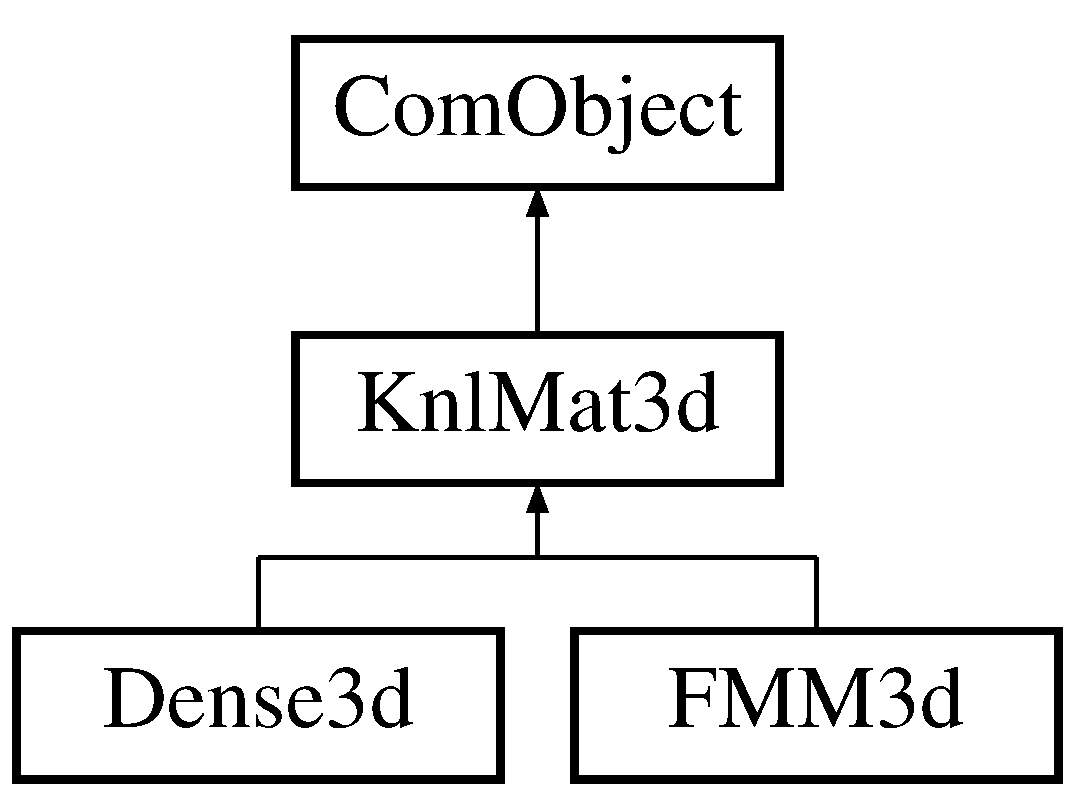
\includegraphics[height=3cm]{classKnlMat3d}
\end{center}
\end{figure}


\subsection{Detailed Description}




Definition at line 26 of file knlmat3d.hpp.\subsection*{Public Member Functions}
\begin{CompactItemize}
\item 
{\bf Knl\-Mat3d} (const string \&p)
\item 
virtual {\bf $\sim$Knl\-Mat3d} ()
\item 
Dbl\-Num\-Mat $\ast$\& {\bf src\-Pos} ()
\item 
Dbl\-Num\-Mat $\ast$\& {\bf src\-Nor} ()
\item 
Dbl\-Num\-Mat $\ast$\& {\bf trg\-Pos} ()
\item 
{\bf Kernel3d} \& {\bf knl} ()
\item 
virtual int {\bf setup} (map$<$ string, string $>$ \&)=0
\item 
virtual int {\bf evaluate} (const Dbl\-Num\-Vec \&src\-Den, Dbl\-Num\-Vec \&trg\-Val)=0
\item 
int {\bf dim} ()
\item 
int {\bf src\-DOF} ()
\item 
int {\bf trg\-DOF} ()
\end{CompactItemize}
\subsection*{Protected Attributes}
\begin{CompactItemize}
\item 
Dbl\-Num\-Mat $\ast$ {\bf \_\-src\-Pos}
\item 
Dbl\-Num\-Mat $\ast$ {\bf \_\-src\-Nor}
\item 
Dbl\-Num\-Mat $\ast$ {\bf \_\-trg\-Pos}
\item 
{\bf Kernel3d} {\bf \_\-knl}
\end{CompactItemize}


\subsection{Constructor \& Destructor Documentation}
\index{KnlMat3d@{Knl\-Mat3d}!KnlMat3d@{KnlMat3d}}
\index{KnlMat3d@{KnlMat3d}!KnlMat3d@{Knl\-Mat3d}}
\subsubsection{\setlength{\rightskip}{0pt plus 5cm}Knl\-Mat3d::Knl\-Mat3d (const string \& {\em p})\hspace{0.3cm}{\tt  [inline]}}\label{classKnlMat3d_e5c3a44fa56c9abf153bdcd2fd4acca6_e5c3a44fa56c9abf153bdcd2fd4acca6}




Definition at line 39 of file knlmat3d.hpp.

\footnotesize\begin{verbatim}39 :  ComObject(p), _srcPos(NULL), _srcNor(NULL), _trgPos(NULL) {;}
\end{verbatim}\normalsize 


\index{KnlMat3d@{Knl\-Mat3d}!~KnlMat3d@{$\sim$KnlMat3d}}
\index{~KnlMat3d@{$\sim$KnlMat3d}!KnlMat3d@{Knl\-Mat3d}}
\subsubsection{\setlength{\rightskip}{0pt plus 5cm}virtual Knl\-Mat3d::$\sim$Knl\-Mat3d ()\hspace{0.3cm}{\tt  [inline, virtual]}}\label{classKnlMat3d_41844e50417d0e54dd36950b66babb7f_41844e50417d0e54dd36950b66babb7f}




Definition at line 40 of file knlmat3d.hpp.

\footnotesize\begin{verbatim}40 { }
\end{verbatim}\normalsize 




\subsection{Member Function Documentation}
\index{KnlMat3d@{Knl\-Mat3d}!dim@{dim}}
\index{dim@{dim}!KnlMat3d@{Knl\-Mat3d}}
\subsubsection{\setlength{\rightskip}{0pt plus 5cm}int Knl\-Mat3d::dim ()\hspace{0.3cm}{\tt  [inline]}}\label{classKnlMat3d_e3f9953141ca7d7525b58c0ff1ef6b1f_e3f9953141ca7d7525b58c0ff1ef6b1f}


return dimension of the kernel matrix/fmm, set to 3 

Definition at line 57 of file knlmat3d.hpp.

Referenced by FMM3d::check(), Dense3d::evaluate(), Dense3d::setup(), FMM3d::src\-Data(), FMM3d::src\-Exa\-Nor(), FMM3d::src\-Exa\-Pos(), FMM3d::trg\-Data(), and FMM3d::trg\-Exa\-Pos().

\footnotesize\begin{verbatim}57 { return 3; }
\end{verbatim}\normalsize 


\index{KnlMat3d@{Knl\-Mat3d}!evaluate@{evaluate}}
\index{evaluate@{evaluate}!KnlMat3d@{Knl\-Mat3d}}
\subsubsection{\setlength{\rightskip}{0pt plus 5cm}virtual int Knl\-Mat3d::evaluate (const Dbl\-Num\-Vec \& {\em src\-Den}, Dbl\-Num\-Vec \& {\em trg\-Val})\hspace{0.3cm}{\tt  [pure virtual]}}\label{classKnlMat3d_fcf3de1e6ce4ee024ef0d320363bd920_fcf3de1e6ce4ee024ef0d320363bd920}


Virtual evaluation function 

Implemented in {\bf Dense3d} {\rm (p.\,\pageref{classDense3d_3d2ce8cfb3d9632d6b69352f1bb5eda2_3d2ce8cfb3d9632d6b69352f1bb5eda2})}, and {\bf FMM3d} {\rm (p.\,\pageref{classFMM3d_3d2ce8cfb3d9632d6b69352f1bb5eda2_3d2ce8cfb3d9632d6b69352f1bb5eda2})}.\index{KnlMat3d@{Knl\-Mat3d}!knl@{knl}}
\index{knl@{knl}!KnlMat3d@{Knl\-Mat3d}}
\subsubsection{\setlength{\rightskip}{0pt plus 5cm}{\bf Kernel3d}\& Knl\-Mat3d::knl ()\hspace{0.3cm}{\tt  [inline]}}\label{classKnlMat3d_d01911fc223ab4bc9604db12f942194e_d01911fc223ab4bc9604db12f942194e}


return kernel 

Definition at line 49 of file knlmat3d.hpp.

References \_\-knl.

\footnotesize\begin{verbatim}49 { return _knl; }
\end{verbatim}\normalsize 


\index{KnlMat3d@{Knl\-Mat3d}!setup@{setup}}
\index{setup@{setup}!KnlMat3d@{Knl\-Mat3d}}
\subsubsection{\setlength{\rightskip}{0pt plus 5cm}virtual int Knl\-Mat3d::setup (map$<$ string, string $>$ \&)\hspace{0.3cm}{\tt  [pure virtual]}}\label{classKnlMat3d_24cbbecf677cd909a522d252feebf2c6_24cbbecf677cd909a522d252feebf2c6}


Virtual setup function 

Implemented in {\bf Dense3d} {\rm (p.\,\pageref{classDense3d_6c9d66eef2ad01ccfea65cb116bf5726_6c9d66eef2ad01ccfea65cb116bf5726})}, and {\bf FMM3d} {\rm (p.\,\pageref{classFMM3d_d134e155a30bcbea9ad038ffcd737ddc_d134e155a30bcbea9ad038ffcd737ddc})}.\index{KnlMat3d@{Knl\-Mat3d}!srcDOF@{srcDOF}}
\index{srcDOF@{srcDOF}!KnlMat3d@{Knl\-Mat3d}}
\subsubsection{\setlength{\rightskip}{0pt plus 5cm}int Knl\-Mat3d::src\-DOF ()\hspace{0.3cm}{\tt  [inline]}}\label{classKnlMat3d_6b422ba557bb24eff82ac7125e206568_6b422ba557bb24eff82ac7125e206568}


return source degrees of freedom 

Definition at line 59 of file knlmat3d.hpp.

References \_\-knl, and Kernel3d::src\-DOF().

Referenced by FMM3d::check(), FMM3d::evaluate(), Dense3d::evaluate(), FMM3d::src\-Data(), and FMM3d::src\-Exa\-Den().

\footnotesize\begin{verbatim}59 { return _knl.srcDOF(); }
\end{verbatim}\normalsize 


\index{KnlMat3d@{Knl\-Mat3d}!srcNor@{srcNor}}
\index{srcNor@{srcNor}!KnlMat3d@{Knl\-Mat3d}}
\subsubsection{\setlength{\rightskip}{0pt plus 5cm}Dbl\-Num\-Mat$\ast$\& Knl\-Mat3d::src\-Nor ()\hspace{0.3cm}{\tt  [inline]}}\label{classKnlMat3d_bba2c6a917421951f1fbe8f69b9a135b_bba2c6a917421951f1fbe8f69b9a135b}


return source normals 

Definition at line 45 of file knlmat3d.hpp.

References \_\-src\-Nor.

\footnotesize\begin{verbatim}45 { return _srcNor; }
\end{verbatim}\normalsize 


\index{KnlMat3d@{Knl\-Mat3d}!srcPos@{srcPos}}
\index{srcPos@{srcPos}!KnlMat3d@{Knl\-Mat3d}}
\subsubsection{\setlength{\rightskip}{0pt plus 5cm}Dbl\-Num\-Mat$\ast$\& Knl\-Mat3d::src\-Pos ()\hspace{0.3cm}{\tt  [inline]}}\label{classKnlMat3d_caa1dae06f56964efa0f778b696dce61_caa1dae06f56964efa0f778b696dce61}


return source positions 

Definition at line 43 of file knlmat3d.hpp.

References \_\-src\-Pos.

\footnotesize\begin{verbatim}43 { return _srcPos; }
\end{verbatim}\normalsize 


\index{KnlMat3d@{Knl\-Mat3d}!trgDOF@{trgDOF}}
\index{trgDOF@{trgDOF}!KnlMat3d@{Knl\-Mat3d}}
\subsubsection{\setlength{\rightskip}{0pt plus 5cm}int Knl\-Mat3d::trg\-DOF ()\hspace{0.3cm}{\tt  [inline]}}\label{classKnlMat3d_ea43c1f768349e86110e4e2d06e38d10_ea43c1f768349e86110e4e2d06e38d10}


return target degrees of freedom 

Definition at line 61 of file knlmat3d.hpp.

References \_\-knl, and Kernel3d::trg\-DOF().

Referenced by FMM3d::check(), FMM3d::evaluate(), Dense3d::evaluate(), FMM3d::trg\-Data(), and FMM3d::trg\-Exa\-Val().

\footnotesize\begin{verbatim}61 { return _knl.trgDOF(); }
\end{verbatim}\normalsize 


\index{KnlMat3d@{Knl\-Mat3d}!trgPos@{trgPos}}
\index{trgPos@{trgPos}!KnlMat3d@{Knl\-Mat3d}}
\subsubsection{\setlength{\rightskip}{0pt plus 5cm}Dbl\-Num\-Mat$\ast$\& Knl\-Mat3d::trg\-Pos ()\hspace{0.3cm}{\tt  [inline]}}\label{classKnlMat3d_7dc770563c182703b1986abb06c6dbbd_7dc770563c182703b1986abb06c6dbbd}


return target positions 

Definition at line 47 of file knlmat3d.hpp.

References \_\-trg\-Pos.

\footnotesize\begin{verbatim}47 { return _trgPos; }
\end{verbatim}\normalsize 




\subsection{Member Data Documentation}
\index{KnlMat3d@{Knl\-Mat3d}!_knl@{\_\-knl}}
\index{_knl@{\_\-knl}!KnlMat3d@{Knl\-Mat3d}}
\subsubsection{\setlength{\rightskip}{0pt plus 5cm}{\bf Kernel3d} {\bf Knl\-Mat3d::\_\-knl}\hspace{0.3cm}{\tt  [protected]}}\label{classKnlMat3d_cb56a4f532a89bc1a51ee17c2434a106_cb56a4f532a89bc1a51ee17c2434a106}


Kernel. See {\bf kernel3d.hpp}{\rm (p.\,\pageref{kernel3d_8hpp})} and {\bf kernel3d.cpp}{\rm (p.\,\pageref{kernel3d_8cpp})} 

Definition at line 37 of file knlmat3d.hpp.

Referenced by Dense3d::evaluate(), knl(), src\-DOF(), FMM3d::Src\-Equ2Dwn\-Chk\_\-dgemv(), FMM3d::Src\-Equ2Trg\-Chk\_\-dgemv(), FMM3d::Src\-Equ2Upw\-Chk\_\-dgemv(), and trg\-DOF().\index{KnlMat3d@{Knl\-Mat3d}!_srcNor@{\_\-srcNor}}
\index{_srcNor@{\_\-srcNor}!KnlMat3d@{Knl\-Mat3d}}
\subsubsection{\setlength{\rightskip}{0pt plus 5cm}Dbl\-Num\-Mat$\ast$ {\bf Knl\-Mat3d::\_\-src\-Nor}\hspace{0.3cm}{\tt  [protected]}}\label{classKnlMat3d_bbeec6db21041e1b277f4755f21047dd_bbeec6db21041e1b277f4755f21047dd}


source normal 

Definition at line 33 of file knlmat3d.hpp.

Referenced by Dense3d::evaluate(), Dense3d::setup(), and src\-Nor().\index{KnlMat3d@{Knl\-Mat3d}!_srcPos@{\_\-srcPos}}
\index{_srcPos@{\_\-srcPos}!KnlMat3d@{Knl\-Mat3d}}
\subsubsection{\setlength{\rightskip}{0pt plus 5cm}Dbl\-Num\-Mat$\ast$ {\bf Knl\-Mat3d::\_\-src\-Pos}\hspace{0.3cm}{\tt  [protected]}}\label{classKnlMat3d_f66b814fdf8eb17df56ff5ff27a368da_f66b814fdf8eb17df56ff5ff27a368da}


source positions 

Definition at line 31 of file knlmat3d.hpp.

Referenced by FMM3d::check(), Dense3d::evaluate(), Dense3d::setup(), and src\-Pos().\index{KnlMat3d@{Knl\-Mat3d}!_trgPos@{\_\-trgPos}}
\index{_trgPos@{\_\-trgPos}!KnlMat3d@{Knl\-Mat3d}}
\subsubsection{\setlength{\rightskip}{0pt plus 5cm}Dbl\-Num\-Mat$\ast$ {\bf Knl\-Mat3d::\_\-trg\-Pos}\hspace{0.3cm}{\tt  [protected]}}\label{classKnlMat3d_a1b44c7c6fd0a38be167c34537b1a508_a1b44c7c6fd0a38be167c34537b1a508}


target position 

Definition at line 35 of file knlmat3d.hpp.

Referenced by FMM3d::check(), Dense3d::setup(), and trg\-Pos().

The documentation for this class was generated from the following file:\begin{CompactItemize}
\item 
fmm3d/{\bf knlmat3d.hpp}\end{CompactItemize}

\section{Let3d Class Reference}
\label{classLet3d}\index{Let3d@{Let3d}}
{\tt \#include $<$let3d.hpp$>$}

Inheritance diagram for Let3d::\begin{figure}[H]
\begin{center}
\leavevmode
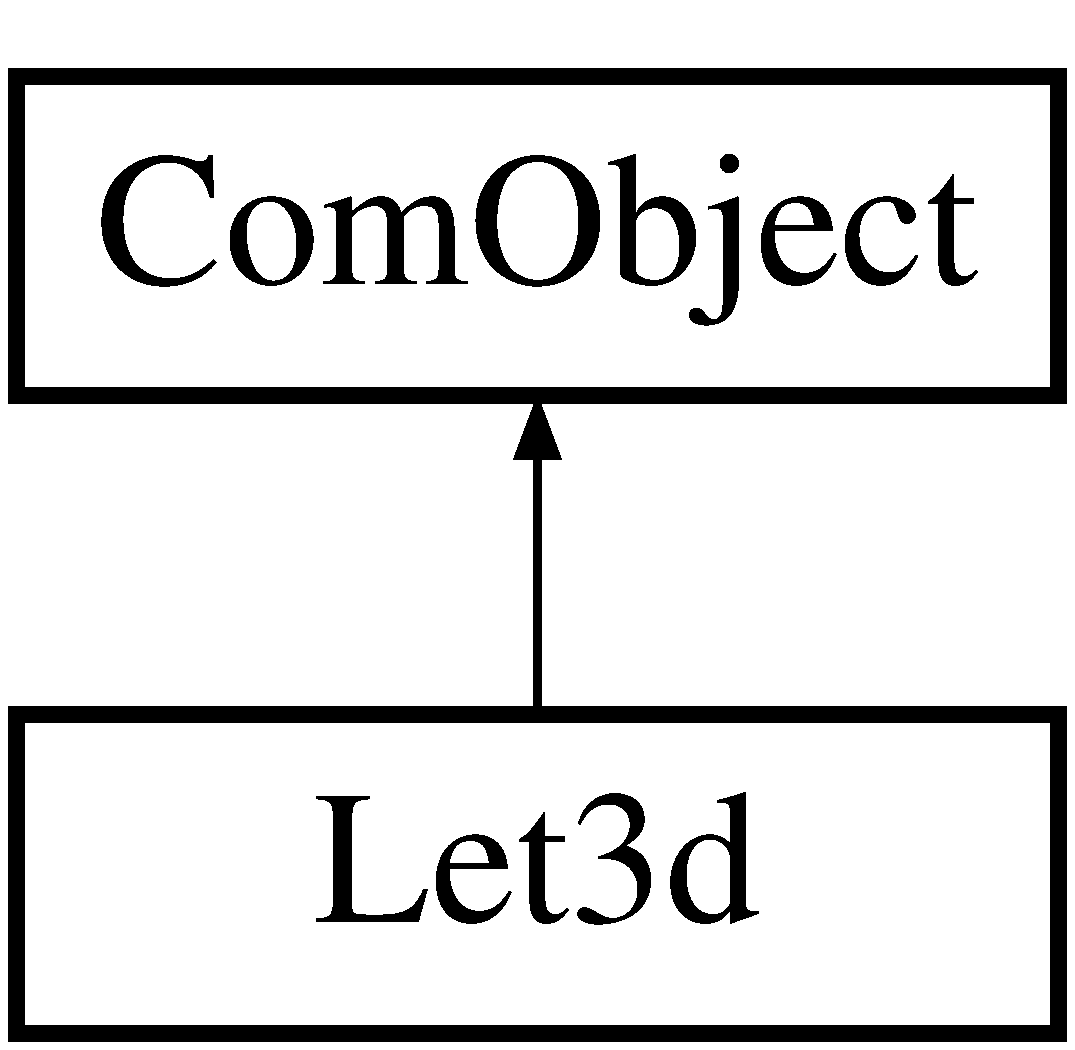
\includegraphics[height=2cm]{classLet3d}
\end{center}
\end{figure}


\subsection{Detailed Description}




Definition at line 34 of file let3d.hpp.\subsection*{Public Member Functions}
\begin{CompactItemize}
\item 
{\bf Let3d} (const string \&p)
\item 
{\bf $\sim$Let3d} ()
\item 
Dbl\-Num\-Mat $\ast$\& {\bf src\-Pos} ()
\item 
Dbl\-Num\-Mat $\ast$\& {\bf trg\-Pos} ()
\item 
Point3 \& {\bf center} ()
\item 
int \& {\bf root\-Level} ()
\item 
double {\bf radius} ()
\item 
int \& {\bf pts\-Max} ()
\item 
int \& {\bf max\-Level} ()
\item 
int {\bf setup} (map$<$ string, string $>$ \&opts)
\item 
int {\bf print} ()
\item 
vector$<$ {\bf Node} $>$ \& {\bf node\-Vec} ()
\item 
int {\bf src\-Node\-Cnt} ()
\item 
int {\bf src\-Exa\-Cnt} ()
\item 
int {\bf trg\-Node\-Cnt} ()
\item 
int {\bf trg\-Exa\-Cnt} ()
\item 
int {\bf src\-Data} ()
\item 
int {\bf trg\-Data} ()
\item 
int {\bf calgnext} (int g\-Node\-Idx)
\item 
int {\bf dwn\-Order\-Collect} (vector$<$ int $>$ \&)
\item 
int {\bf upw\-Order\-Collect} (vector$<$ int $>$ \&)
\item 
{\bf Node} \& {\bf node} (int g\-Node\-Idx)
\item 
bool {\bf root} (int g\-Node\-Idx)
\item 
bool {\bf terminal} (int g\-Node\-Idx)
\item 
int {\bf parent} (int g\-Node\-Idx)
\item 
int {\bf child} (int g\-Node\-Idx, const Index3 \&idx)
\item 
Index3 {\bf path2Node} (int g\-Node\-Idx)
\item 
int {\bf depth} (int g\-Node\-Idx)
\item 
int {\bf tag} (int g\-Node\-Idx)
\item 
Point3 {\bf center} (int g\-Node\-Idx)
\item 
double {\bf radius} (int g\-Node\-Idx)
\item 
int {\bf findgnt} (int depth, const Index3 \&path2Node)
\item 
bool {\bf adjacent} (int, int)
\item 
int {\bf dim} () const 
\end{CompactItemize}
\subsection*{Protected Attributes}
\begin{CompactItemize}
\item 
Dbl\-Num\-Mat $\ast$ {\bf \_\-src\-Pos}
\item 
Dbl\-Num\-Mat $\ast$ {\bf \_\-trg\-Pos}
\item 
Point3 {\bf \_\-center}
\item 
int {\bf \_\-root\-Level}
\item 
int {\bf \_\-pts\-Max}
\item 
int {\bf \_\-max\-Level}
\item 
vector$<$ {\bf Node} $>$ {\bf \_\-node\-Vec}
\item 
int {\bf \_\-level}
\item 
int {\bf \_\-src\-Node\-Cnt}
\item 
int {\bf \_\-src\-Exa\-Cnt}
\item 
int {\bf \_\-trg\-Node\-Cnt}
\item 
int {\bf \_\-trg\-Exa\-Cnt}
\end{CompactItemize}
\subsection*{Classes}
\begin{CompactItemize}
\item 
class {\bf Node}
\end{CompactItemize}


\subsection{Constructor \& Destructor Documentation}
\index{Let3d@{Let3d}!Let3d@{Let3d}}
\index{Let3d@{Let3d}!Let3d@{Let3d}}
\subsubsection{\setlength{\rightskip}{0pt plus 5cm}Let3d::Let3d (const string \& {\em p})}\label{classLet3d_f8d536a83eec83f76c37ef8ab65ca50a_f8d536a83eec83f76c37ef8ab65ca50a}




Definition at line 30 of file let3d.cpp.

\footnotesize\begin{verbatim}30                            :
31   ComObject(p), _srcPos(NULL), _trgPos(NULL), _center(0.0), _rootLevel(0),
32   _ptsMax(150), _maxLevel(10)
33 {
34 }

\end{verbatim}\normalsize 


\index{Let3d@{Let3d}!~Let3d@{$\sim$Let3d}}
\index{~Let3d@{$\sim$Let3d}!Let3d@{Let3d}}
\subsubsection{\setlength{\rightskip}{0pt plus 5cm}Let3d::$\sim$Let3d ()}\label{classLet3d_b2dea69683e4c627d67f9de0f72909c1_b2dea69683e4c627d67f9de0f72909c1}




Definition at line 36 of file let3d.cpp.

\footnotesize\begin{verbatim}37 {
38 }
\end{verbatim}\normalsize 




\subsection{Member Function Documentation}
\index{Let3d@{Let3d}!adjacent@{adjacent}}
\index{adjacent@{adjacent}!Let3d@{Let3d}}
\subsubsection{\setlength{\rightskip}{0pt plus 5cm}bool Let3d::adjacent (int, int)}\label{classLet3d_a20d0c310a6e8d02f6295983c199c06f_a20d0c310a6e8d02f6295983c199c06f}




Definition at line 372 of file let3d.cpp.

References depth(), path2Node(), and radius().

Referenced by calgnext().

\footnotesize\begin{verbatim}373 {
374   int md = max(depth(me),depth(yo));
375   Index3 one(1);
376   Index3 mecenter(  (2*path2Node(me)+one) * pow2(md - depth(me))  );
377   Index3 yocenter(  (2*path2Node(yo)+one) * pow2(md - depth(yo))  );
378   int meradius = pow2(md - depth(me));
379   int yoradius = pow2(md - depth(yo));
380   Index3 dif( abs(mecenter-yocenter) );
381   int radius  = meradius + yoradius;
382   return
383          ( dif <= Index3(radius) ) && //not too far
384          ( dif.linfty() == radius ); //at least one edge touch
385 }
\end{verbatim}\normalsize 


\index{Let3d@{Let3d}!calgnext@{calgnext}}
\index{calgnext@{calgnext}!Let3d@{Let3d}}
\subsubsection{\setlength{\rightskip}{0pt plus 5cm}int Let3d::calgnext (int {\em g\-Node\-Idx})}\label{classLet3d_a57baa80b52cce7a3e0430c3bd3e6107_a57baa80b52cce7a3e0430c3bd3e6107}


build U,V,W,X lists 

Definition at line 234 of file let3d.cpp.

References adjacent(), depth(), findgnt(), node\-Vec(), parent(), path2Node(), root(), and terminal().

\footnotesize\begin{verbatim}235 {
236   vector<Node>&  nodeVec = this->nodeVec();
237   
238   set<int> Uset, Vset, Wset, Xset;
239   int curGNodeIdx = gNodeIdx;
240   if(root(curGNodeIdx)==false) {
241          int parGNodeIdx = parent(curGNodeIdx);
242          
243          Index3 minIdx(0);
244          Index3 maxIdx(pow2(depth(curGNodeIdx)));
245 
246          for(int i=-2; i<4; i++) {
247                 for(int j=-2; j<4; j++) {
248                   for(int k=-2; k<4; k++) {
249                          Index3 tryPath( 2*path2Node(parGNodeIdx) + Index3(i,j,k) );
250                          if(tryPath >= minIdx && tryPath <  maxIdx && tryPath != path2Node(curGNodeIdx)) {      
251                                 int resGNodeIdx = findgnt(depth(curGNodeIdx), tryPath);
252                                 bool adj = adjacent(resGNodeIdx, curGNodeIdx);
253                                 if( depth(resGNodeIdx) < depth(curGNodeIdx) ) {
254                                   if(adj){
255                                          if(terminal(curGNodeIdx)){
256                                                 Uset.insert(resGNodeIdx);
257                                          }
258                                          else { ; }
259                                   }
260                                   else {
261                                          Xset.insert(resGNodeIdx);
262                                   }
263                                 }
264                                 if( depth(resGNodeIdx)==depth(curGNodeIdx) ) {
265                                   if(!adj) {
266                                          Index3 bb(path2Node(resGNodeIdx)-path2Node(curGNodeIdx));
267                                          assert( bb.linfty()<=3 );
268                                          Vset.insert(resGNodeIdx);
269                                   }
270                                   else {
271                                          if(terminal(curGNodeIdx)) {
272                                                 queue<int> rest;
273                                                 rest.push(resGNodeIdx);
274                                                 while(rest.empty()==false) {
275                                                   int fntGNodeIdx = rest.front(); rest.pop();                                    //int fntgNodeIdx = fntgnt.gNodeIdx();
276                                                   if(adjacent(fntGNodeIdx, curGNodeIdx)==false) {
277                                                          Wset.insert( fntGNodeIdx );
278                                                   }
279                                                   else {
280                                                          if(terminal(fntGNodeIdx)) {
281                                                                 Uset.insert(fntGNodeIdx);
282                                                          }
283                                                          else { 
284                                                                 for(int a=0; a<2; a++) {
285                                                                   for(int b=0; b<2; b++) {
286                                                                          for(int c=0; c<2; c++) {
287                                                                                 rest.push( child(fntGNodeIdx, Index3(a,b,c)) );
288                                                                          }
289                                                                   }
290                                                                 }
291                                                          }
292                                                   }
293                                                 }
294                                          }
295                                   }
296                                 }
297                          }
298                   }
299                 }
300          }
301   }
302   if(terminal(curGNodeIdx))
303          Uset.insert(curGNodeIdx);
304   
305   for(set<int>::iterator si=Uset.begin(); si!=Uset.end(); si++)
306          if(nodeVec[*si].tag() & LET_SRCNODE)           nodeVec[gNodeIdx].Unodes().push_back(*si);
307   for(set<int>::iterator si=Vset.begin(); si!=Vset.end(); si++)
308          if(nodeVec[*si].tag() & LET_SRCNODE)           nodeVec[gNodeIdx].Vnodes().push_back(*si);
309   for(set<int>::iterator si=Wset.begin(); si!=Wset.end(); si++)
310          if(nodeVec[*si].tag() & LET_SRCNODE)           nodeVec[gNodeIdx].Wnodes().push_back(*si);
311   for(set<int>::iterator si=Xset.begin(); si!=Xset.end(); si++)
312          if(nodeVec[*si].tag() & LET_SRCNODE)           nodeVec[gNodeIdx].Xnodes().push_back(*si);
313   
314   return (0);
315 }
\end{verbatim}\normalsize 


\index{Let3d@{Let3d}!center@{center}}
\index{center@{center}!Let3d@{Let3d}}
\subsubsection{\setlength{\rightskip}{0pt plus 5cm}Point3 Let3d::center (int {\em g\-Node\-Idx})}\label{classLet3d_dff5f922c11176af18f4bfa95c138a20_dff5f922c11176af18f4bfa95c138a20}




Definition at line 342 of file let3d.cpp.

References center(), depth(), dim(), path2Node(), and radius().

\footnotesize\begin{verbatim}343 {
344   Point3 ll( center() - Point3(radius()) );
345   int tmp = pow2(depth(gNodeIdx));
346   Index3 pathLcl(path2Node(gNodeIdx));
347   Point3 res;
348   for(int d=0; d<dim(); d++) {
349          res(d) = ll(d) + (2*radius()) * (pathLcl(d)+0.5) / double(tmp);
350   }
351   return res;
352 }
\end{verbatim}\normalsize 


\index{Let3d@{Let3d}!center@{center}}
\index{center@{center}!Let3d@{Let3d}}
\subsubsection{\setlength{\rightskip}{0pt plus 5cm}Point3\& Let3d::center ()\hspace{0.3cm}{\tt  [inline]}}\label{classLet3d_5c0517b22b09f08712cbfd01aa1f29d7_5c0517b22b09f08712cbfd01aa1f29d7}




Definition at line 122 of file let3d.hpp.

References \_\-center.

Referenced by center(), src\-Data(), and trg\-Data().

\footnotesize\begin{verbatim}122 { return _center; }
\end{verbatim}\normalsize 


\index{Let3d@{Let3d}!child@{child}}
\index{child@{child}!Let3d@{Let3d}}
\subsubsection{\setlength{\rightskip}{0pt plus 5cm}int Let3d::child (int {\em g\-Node\-Idx}, const Index3 \& {\em idx})}\label{classLet3d_127278ccf71ca1d7a807d7531be1ad40_127278ccf71ca1d7a807d7531be1ad40}




Definition at line 337 of file let3d.cpp.

References Let3d::Node::child(), and node().

Referenced by findgnt().

\footnotesize\begin{verbatim}338 {
339   assert(idx>=Index3(0) && idx<Index3(2));
340   return node(gNodeIdx).child() + (idx(0)*4+idx(1)*2+idx(2));
341 }
\end{verbatim}\normalsize 


\index{Let3d@{Let3d}!depth@{depth}}
\index{depth@{depth}!Let3d@{Let3d}}
\subsubsection{\setlength{\rightskip}{0pt plus 5cm}int Let3d::depth (int {\em g\-Node\-Idx})\hspace{0.3cm}{\tt  [inline]}}\label{classLet3d_365114de1453e803d05b02702d1e0bc2_365114de1453e803d05b02702d1e0bc2}




Definition at line 156 of file let3d.hpp.

References Let3d::Node::depth(), and node().

Referenced by adjacent(), calgnext(), center(), findgnt(), and radius().

\footnotesize\begin{verbatim}156 { return node(gNodeIdx).depth(); }
\end{verbatim}\normalsize 


\index{Let3d@{Let3d}!dim@{dim}}
\index{dim@{dim}!Let3d@{Let3d}}
\subsubsection{\setlength{\rightskip}{0pt plus 5cm}int Let3d::dim () const\hspace{0.3cm}{\tt  [inline]}}\label{classLet3d_3b54adb16617f4dccdd399f842f3f6bf_3b54adb16617f4dccdd399f842f3f6bf}




Definition at line 165 of file let3d.hpp.

Referenced by center(), src\-Data(), and trg\-Data().

\footnotesize\begin{verbatim}165 { return 3; }  
\end{verbatim}\normalsize 


\index{Let3d@{Let3d}!dwnOrderCollect@{dwnOrderCollect}}
\index{dwnOrderCollect@{dwnOrderCollect}!Let3d@{Let3d}}
\subsubsection{\setlength{\rightskip}{0pt plus 5cm}int Let3d::dwn\-Order\-Collect (vector$<$ int $>$ \&)}\label{classLet3d_1917ece529ea97f12e74e56e42b6d15a_1917ece529ea97f12e74e56e42b6d15a}


top down ordering of the nodes 

Definition at line 317 of file let3d.cpp.

References \_\-\_\-FUNCT\_\-\_\-, and node\-Vec().

\footnotesize\begin{verbatim}318 {
319   orderBoxesVec.clear();
320   for(int i=0; i < nodeVec().size(); i++)
321          orderBoxesVec.push_back(i);
322   iA(orderBoxesVec.size()==nodeVec().size());
323   return 0;
324 }
\end{verbatim}\normalsize 


\index{Let3d@{Let3d}!findgnt@{findgnt}}
\index{findgnt@{findgnt}!Let3d@{Let3d}}
\subsubsection{\setlength{\rightskip}{0pt plus 5cm}int Let3d::findgnt (int {\em depth}, const Index3 \& {\em path2Node})}\label{classLet3d_dadf07c3ca29b244d01e8570e2846a2c_dadf07c3ca29b244d01e8570e2846a2c}




Definition at line 358 of file let3d.cpp.

References child(), depth(), and terminal().

Referenced by calgnext().

\footnotesize\begin{verbatim}359 {
360   int cur = 0;  //cerr<<"GOOD "<<path(cur)<<"     ";
361   Index3 leftpath(wntpath);
362   while(depth(cur)<wntdepth && terminal(cur)==false) {
363          int dif = wntdepth-depth(cur);
364          int tmp = pow2(dif-1);
365          Index3 choice( leftpath/tmp );
366          leftpath -= choice*tmp;
367          cur = child(cur, choice);       //cur = child(cur, IdxIter(0,2,true,choice) );  //cerr<<path(cur)<<"["<<choice<<" "<<tmp<<"]"<<"     ";
368   }  //cerr<<endl;
369   return cur;
370 }
\end{verbatim}\normalsize 


\index{Let3d@{Let3d}!maxLevel@{maxLevel}}
\index{maxLevel@{maxLevel}!Let3d@{Let3d}}
\subsubsection{\setlength{\rightskip}{0pt plus 5cm}int\& Let3d::max\-Level ()\hspace{0.3cm}{\tt  [inline]}}\label{classLet3d_fdc3ca03e415e2d7b0b1f708d3ab94bb_fdc3ca03e415e2d7b0b1f708d3ab94bb}




Definition at line 126 of file let3d.hpp.

References \_\-max\-Level.

\footnotesize\begin{verbatim}126 { return _maxLevel; }
\end{verbatim}\normalsize 


\index{Let3d@{Let3d}!node@{node}}
\index{node@{node}!Let3d@{Let3d}}
\subsubsection{\setlength{\rightskip}{0pt plus 5cm}{\bf Node}\& Let3d::node (int {\em g\-Node\-Idx})\hspace{0.3cm}{\tt  [inline]}}\label{classLet3d_f259ccf218dbf0a04530841785f1a8b0_f259ccf218dbf0a04530841785f1a8b0}


node access 

Definition at line 148 of file let3d.hpp.

References \_\-node\-Vec.

Referenced by child(), depth(), FMM3d::evaluate(), parent(), path2Node(), print(), root(), FMM3d::src\-Data(), FMM3d::src\-Exa\-Den(), FMM3d::src\-Exa\-Nor(), FMM3d::src\-Exa\-Pos(), FMM3d::src\-Upw\-Chk\-Val(), FMM3d::src\-Upw\-Equ\-Den(), tag(), terminal(), FMM3d::trg\-Data(), FMM3d::trg\-Dwn\-Chk\-Val(), FMM3d::trg\-Dwn\-Equ\-Den(), FMM3d::trg\-Exa\-Pos(), and FMM3d::trg\-Exa\-Val().

\footnotesize\begin{verbatim}148 { return _nodeVec[gNodeIdx]; }
\end{verbatim}\normalsize 


\index{Let3d@{Let3d}!nodeVec@{nodeVec}}
\index{nodeVec@{nodeVec}!Let3d@{Let3d}}
\subsubsection{\setlength{\rightskip}{0pt plus 5cm}vector$<${\bf Node}$>$\& Let3d::node\-Vec ()\hspace{0.3cm}{\tt  [inline]}}\label{classLet3d_44c0c8da466878274feb4ce060c10b9b_44c0c8da466878274feb4ce060c10b9b}




Definition at line 131 of file let3d.hpp.

References \_\-node\-Vec.

Referenced by calgnext(), dwn\-Order\-Collect(), src\-Data(), trg\-Data(), FMM3d::trg\-Data(), and upw\-Order\-Collect().

\footnotesize\begin{verbatim}131 { return _nodeVec; }
\end{verbatim}\normalsize 


\index{Let3d@{Let3d}!parent@{parent}}
\index{parent@{parent}!Let3d@{Let3d}}
\subsubsection{\setlength{\rightskip}{0pt plus 5cm}int Let3d::parent (int {\em g\-Node\-Idx})\hspace{0.3cm}{\tt  [inline]}}\label{classLet3d_eedcae6652a6a95ae0ef366d7e8ad0ef_eedcae6652a6a95ae0ef366d7e8ad0ef}




Definition at line 153 of file let3d.hpp.

References node(), and Let3d::Node::parent().

Referenced by calgnext().

\footnotesize\begin{verbatim}153 { assert(node(gNodeIdx).parent()!=-1); return node(gNodeIdx).parent(); }
\end{verbatim}\normalsize 


\index{Let3d@{Let3d}!path2Node@{path2Node}}
\index{path2Node@{path2Node}!Let3d@{Let3d}}
\subsubsection{\setlength{\rightskip}{0pt plus 5cm}Index3 Let3d::path2Node (int {\em g\-Node\-Idx})\hspace{0.3cm}{\tt  [inline]}}\label{classLet3d_8df44bec9d337d228d001b12e5e6379e_8df44bec9d337d228d001b12e5e6379e}




Definition at line 155 of file let3d.hpp.

References node(), and Let3d::Node::path2Node().

Referenced by adjacent(), calgnext(), and center().

\footnotesize\begin{verbatim}155 { return node(gNodeIdx).path2Node(); }
\end{verbatim}\normalsize 


\index{Let3d@{Let3d}!print@{print}}
\index{print@{print}!Let3d@{Let3d}}
\subsubsection{\setlength{\rightskip}{0pt plus 5cm}int Let3d::print ()}\label{classLet3d_d0d33c63402dfb2c02713a7fd52578c1_d0d33c63402dfb2c02713a7fd52578c1}




Definition at line 388 of file let3d.cpp.

References \_\-level, \_\-node\-Vec, \_\-src\-Exa\-Cnt, \_\-src\-Node\-Cnt, \_\-trg\-Exa\-Cnt, \_\-trg\-Node\-Cnt, Let3d::Node::child(), node(), and Let3d::Node::parent().

\footnotesize\begin{verbatim}389 {
390   cerr<<_nodeVec.size()<<" "<<_level<<endl;
391   cerr<<_srcNodeCnt <<" "<< _srcExaCnt << endl;
392   cerr<<_trgNodeCnt <<" "<< _trgExaCnt << endl;
393 
394   for(int i=0; i<_nodeVec.size(); i++) {
395          cerr<<node(i).parent()<<" "<<node(i).child()<<endl;
396   }
397   
398   for(int i=0; i<_nodeVec.size(); i++) {
399          //cerr<<node(i).Unodes().size()<<" "<<node(i).Vnodes().size()<<" "<<node(i).Wnodes().size()<<" "<<node(i).Xnodes().size()<<" "<<endl;
400          Node& n = node(i);
401          cerr<<n.srcNodeIdx()<<" "<<n.srcExaBeg()<<" "<<n.srcExaNum()<<" "
402                   <<n.trgNodeIdx()<<" "<<n.trgExaBeg()<<" "<<n.trgExaNum()<<endl;
403   }
404   return 0;
405 }
\end{verbatim}\normalsize 


\index{Let3d@{Let3d}!ptsMax@{ptsMax}}
\index{ptsMax@{ptsMax}!Let3d@{Let3d}}
\subsubsection{\setlength{\rightskip}{0pt plus 5cm}int\& Let3d::pts\-Max ()\hspace{0.3cm}{\tt  [inline]}}\label{classLet3d_682c29880d87862bd529f951970bf83a_682c29880d87862bd529f951970bf83a}




Definition at line 125 of file let3d.hpp.

References \_\-pts\-Max.

\footnotesize\begin{verbatim}125 { return _ptsMax; }
\end{verbatim}\normalsize 


\index{Let3d@{Let3d}!radius@{radius}}
\index{radius@{radius}!Let3d@{Let3d}}
\subsubsection{\setlength{\rightskip}{0pt plus 5cm}double Let3d::radius (int {\em g\-Node\-Idx})}\label{classLet3d_c1534d5f7ba6030886668befb2b472c0_c1534d5f7ba6030886668befb2b472c0}




Definition at line 353 of file let3d.cpp.

References depth(), and radius().

\footnotesize\begin{verbatim}354 {
355   return radius()/double(pow2(depth(gNodeIdx)));
356 }
\end{verbatim}\normalsize 


\index{Let3d@{Let3d}!radius@{radius}}
\index{radius@{radius}!Let3d@{Let3d}}
\subsubsection{\setlength{\rightskip}{0pt plus 5cm}double Let3d::radius ()\hspace{0.3cm}{\tt  [inline]}}\label{classLet3d_703550342372334b492a37f2f4379409_703550342372334b492a37f2f4379409}




Definition at line 124 of file let3d.hpp.

References \_\-root\-Level.

Referenced by adjacent(), center(), radius(), src\-Data(), and trg\-Data().

\footnotesize\begin{verbatim}124 { return pow(2.0, -_rootLevel); }
\end{verbatim}\normalsize 


\index{Let3d@{Let3d}!root@{root}}
\index{root@{root}!Let3d@{Let3d}}
\subsubsection{\setlength{\rightskip}{0pt plus 5cm}bool Let3d::root (int {\em g\-Node\-Idx})\hspace{0.3cm}{\tt  [inline]}}\label{classLet3d_06ef4c5a5a60303ba9b0b041a8bb5000_06ef4c5a5a60303ba9b0b041a8bb5000}




Definition at line 151 of file let3d.hpp.

References node(), and Let3d::Node::parent().

Referenced by calgnext().

\footnotesize\begin{verbatim}151 { return node(gNodeIdx).parent()==-1; } //no parent
\end{verbatim}\normalsize 


\index{Let3d@{Let3d}!rootLevel@{rootLevel}}
\index{rootLevel@{rootLevel}!Let3d@{Let3d}}
\subsubsection{\setlength{\rightskip}{0pt plus 5cm}int\& Let3d::root\-Level ()\hspace{0.3cm}{\tt  [inline]}}\label{classLet3d_f80fcb36cb42936f1912fe8c85ec96e4_f80fcb36cb42936f1912fe8c85ec96e4}




Definition at line 123 of file let3d.hpp.

References \_\-root\-Level.

\footnotesize\begin{verbatim}123 { return _rootLevel; }
\end{verbatim}\normalsize 


\index{Let3d@{Let3d}!setup@{setup}}
\index{setup@{setup}!Let3d@{Let3d}}
\subsubsection{\setlength{\rightskip}{0pt plus 5cm}int Let3d::setup (map$<$ string, string $>$ \& {\em opts})}\label{classLet3d_d134e155a30bcbea9ad038ffcd737ddc_d134e155a30bcbea9ad038ffcd737ddc}




Definition at line 41 of file let3d.cpp.

References \_\-pts\-Max, and Com\-Object::prefix().

\footnotesize\begin{verbatim}42 {
43   //------------
44   map<string,string>::iterator mapindex;
45   mapindex = optionsMap.find("-" + prefix() + "ptsMax"); iA(mapindex!=optionsMap.end());
46   { istringstream ss((*mapindex).second); ss>>_ptsMax; }
47   mapindex = optionsMap.find("-" + prefix() + "maxLevel"); iA(mapindex!=optionsMap.end());
48   { istringstream ss((*mapindex).second); ss>>_maxLevel; }
49   //------------
50   iC( srcData() );
51   iC( trgData() );
52   return 0;
53 }
\end{verbatim}\normalsize 


\index{Let3d@{Let3d}!srcData@{srcData}}
\index{srcData@{srcData}!Let3d@{Let3d}}
\subsubsection{\setlength{\rightskip}{0pt plus 5cm}int Let3d::src\-Data ()}\label{classLet3d_44ef9057a3adc0372c2569c172064dac_44ef9057a3adc0372c2569c172064dac}


gdata 

Definition at line 56 of file let3d.cpp.

References \_\-src\-Pos, center(), dim(), node\-Vec(), and radius().

\footnotesize\begin{verbatim}57 {
58   //-----------------------------------------
60   DblNumMat& pos = *(_srcPos);  iA( pos.m()==dim() );
61   
62   vector<Node>& nodeVec = this->nodeVec(); nodeVec.clear();
63   vector< vector<int> > vecIdxs;  
64   //local src number, the number of src point in each box
65   vector<int> lclSrcNumVec; //glb 
66   
67   nodeVec.push_back( Node(-1,-1, Index3(0,0,0), 0) );
68   vecIdxs.push_back( vector<int>() );
69   vector<int>& curVecIdxs = vecIdxs[0];
70   Point3 bbmin(center()-Point3(radius()));
71   Point3 bbmax(center()+Point3(radius()));
72   for(int k=0; k<pos.n(); k++) {
73          Point3 tmp(pos.clmdata(k));     
74          iA(tmp>=bbmin && tmp<=bbmax);//LEXING: IMPORANT
75          curVecIdxs.push_back(k);
76   }
77   lclSrcNumVec.push_back( curVecIdxs.size() );
78   
79   int level = 0;
80   int arrBeg = 0;
81   int arrEnd = 1;
82   int arrCnt = 0;
83   while(arrBeg < arrEnd) {
84          //1.
85          arrCnt = arrEnd;
86          for(int k=arrBeg; k < arrEnd; k++) {
87                 //---
88                 if( lclSrcNumVec[k]>ptsMax() && level<maxLevel()-1 ) {
89                   nodeVec[k].child() = arrCnt;
90                   arrCnt = arrCnt + pow2(dim());
91                   //children's ess                
92                   for(int a=0; a<2; a++) {
93                          for(int b=0; b<2; b++) {
94                                 for(int c=0; c<2; c++) {
95                                   nodeVec.push_back( Node(k,-1, 2*nodeVec[k].path2Node()+Index3(a,b,c), nodeVec[k].depth()+1) ); //par, chd
96                                   vecIdxs.push_back( vector<int>() );
97                                   lclSrcNumVec.push_back( 0 );
98                                 }
99                          }
100                   }
101                   //children's vector of indices
102                   Point3 centerCurNode( center(k) ); //get center of current node
103                   for(vector<int>::iterator vecIdxsIt=vecIdxs[k].begin(); vecIdxsIt!=vecIdxs[k].end(); vecIdxsIt++) {
104                          Point3 tmp(pos.clmdata(*vecIdxsIt));
105                          Index3 idx;
106                          for(int j=0; j<dim(); j++){
107                                 idx(j) = (tmp(j) >= centerCurNode(j));
108                          }
109                          int chdGNodeIdx = child(k, idx);
110                          vecIdxs[chdGNodeIdx].push_back(*vecIdxsIt);
111                   }
112                   vecIdxs[k].clear(); //VERY IMPORTANT
113                   //children's lsm                
114                   for(int a=0; a<2; a++) {
115                          for(int b=0; b<2; b++) {
116                                 for(int c=0; c<2; c++) {
117                                   int chdGNodeIdx = child( k, Index3(a,b,c) );
118                                   lclSrcNumVec[chdGNodeIdx] = vecIdxs[chdGNodeIdx].size();
119                                 }
120                          }
121                   }
122                 }
123          }
124          level++;
125          arrBeg = arrEnd;
126          arrEnd = arrCnt;
127   }
128   _level = level; //SET LEVEL
129 
130   //ordering of the boxes, in top-down or bottom-up fashion
131   vector<int> orderBoxesVec     ;  iC( dwnOrderCollect(orderBoxesVec    ) );
132   //set other parts of essvec
133   int cnt = 0;
134   int sum = 0;
135   for(int i=0; i < orderBoxesVec        .size(); i++) {
136          int gNodeIdx = orderBoxesVec   [i];
137          if(lclSrcNumVec[gNodeIdx]>0) {
138                 nodeVec[gNodeIdx].tag() = nodeVec[gNodeIdx].tag() | LET_SRCNODE;
139                 nodeVec[gNodeIdx].srcNodeIdx() = cnt;
140                 cnt++;
141                 if(nodeVec[gNodeIdx].child()==-1) {
142                   nodeVec[gNodeIdx].srcExaBeg() = sum;
143                   nodeVec[gNodeIdx].srcExaNum() = lclSrcNumVec[gNodeIdx];
144                   sum += lclSrcNumVec[gNodeIdx];
145                   nodeVec[gNodeIdx].srcOwnVecIdxs() = vecIdxs[gNodeIdx];
146                 }
147          }
148   }
149   _srcNodeCnt = cnt;  _srcExaCnt = sum; //SET S cnts
150   return 0;
151 }
\end{verbatim}\normalsize 


\index{Let3d@{Let3d}!srcExaCnt@{srcExaCnt}}
\index{srcExaCnt@{srcExaCnt}!Let3d@{Let3d}}
\subsubsection{\setlength{\rightskip}{0pt plus 5cm}int Let3d::src\-Exa\-Cnt ()\hspace{0.3cm}{\tt  [inline]}}\label{classLet3d_634dbea010c08e20a4029d6c0c4550e3_634dbea010c08e20a4029d6c0c4550e3}




Definition at line 133 of file let3d.hpp.

References \_\-src\-Exa\-Cnt.

Referenced by FMM3d::src\-Data().

\footnotesize\begin{verbatim}133 { return _srcExaCnt; }
\end{verbatim}\normalsize 


\index{Let3d@{Let3d}!srcNodeCnt@{srcNodeCnt}}
\index{srcNodeCnt@{srcNodeCnt}!Let3d@{Let3d}}
\subsubsection{\setlength{\rightskip}{0pt plus 5cm}int Let3d::src\-Node\-Cnt ()\hspace{0.3cm}{\tt  [inline]}}\label{classLet3d_69b43bb5940038243065dc6bc4ad0fcb_69b43bb5940038243065dc6bc4ad0fcb}




Definition at line 132 of file let3d.hpp.

References \_\-src\-Node\-Cnt.

Referenced by FMM3d::src\-Data().

\footnotesize\begin{verbatim}132 { return _srcNodeCnt; }
\end{verbatim}\normalsize 


\index{Let3d@{Let3d}!srcPos@{srcPos}}
\index{srcPos@{srcPos}!Let3d@{Let3d}}
\subsubsection{\setlength{\rightskip}{0pt plus 5cm}Dbl\-Num\-Mat$\ast$\& Let3d::src\-Pos ()\hspace{0.3cm}{\tt  [inline]}}\label{classLet3d_caa1dae06f56964efa0f778b696dce61_caa1dae06f56964efa0f778b696dce61}




Definition at line 120 of file let3d.hpp.

References \_\-src\-Pos.

\footnotesize\begin{verbatim}120 { return _srcPos; }
\end{verbatim}\normalsize 


\index{Let3d@{Let3d}!tag@{tag}}
\index{tag@{tag}!Let3d@{Let3d}}
\subsubsection{\setlength{\rightskip}{0pt plus 5cm}int Let3d::tag (int {\em g\-Node\-Idx})\hspace{0.3cm}{\tt  [inline]}}\label{classLet3d_07c220944caf5b6aa5c5454c42d18753_07c220944caf5b6aa5c5454c42d18753}




Definition at line 157 of file let3d.hpp.

References node(), and Let3d::Node::tag().

Referenced by FMM3d::evaluate(), FMM3d::src\-Data(), and FMM3d::trg\-Data().

\footnotesize\begin{verbatim}157 { return node(gNodeIdx).tag(); }
\end{verbatim}\normalsize 


\index{Let3d@{Let3d}!terminal@{terminal}}
\index{terminal@{terminal}!Let3d@{Let3d}}
\subsubsection{\setlength{\rightskip}{0pt plus 5cm}bool Let3d::terminal (int {\em g\-Node\-Idx})\hspace{0.3cm}{\tt  [inline]}}\label{classLet3d_8bef6e640d1f466fdac02445bb2873ef_8bef6e640d1f466fdac02445bb2873ef}




Definition at line 152 of file let3d.hpp.

References Let3d::Node::child(), and node().

Referenced by calgnext(), FMM3d::evaluate(), findgnt(), FMM3d::src\-Data(), and FMM3d::trg\-Data().

\footnotesize\begin{verbatim}152 { return node(gNodeIdx).child()==-1; } //no child
\end{verbatim}\normalsize 


\index{Let3d@{Let3d}!trgData@{trgData}}
\index{trgData@{trgData}!Let3d@{Let3d}}
\subsubsection{\setlength{\rightskip}{0pt plus 5cm}int Let3d::trg\-Data ()}\label{classLet3d_ca481263feff458d83769363d3ad85f7_ca481263feff458d83769363d3ad85f7}




Definition at line 154 of file let3d.cpp.

References \_\-trg\-Pos, center(), dim(), node\-Vec(), and radius().

\footnotesize\begin{verbatim}155 {
156   //-----------------------------------------
157   //edata
158   DblNumMat& pos = *(_trgPos);  iA( pos.m()==dim() );
159   
160   vector<Node>& nodeVec = this->nodeVec();
161   vector< vector<int> > vecIdxs; vecIdxs.resize(nodeVec.size() );
162   vector<int> lclSrcNumVec;           lclSrcNumVec.resize(nodeVec.size(), 0);
163   
164   vector<int>& curVecIdxs = vecIdxs[0];
165   Point3 bbmin(center()-Point3(radius()));
166   Point3 bbmax(center()+Point3(radius()));  //cerr<<" bbx "<<bbmin<<" "<<bbmax<<endl;
167   for(int k=0; k < pos.n(); k++) {
168          Point3 tmp(pos.clmdata(k));
169          iA(tmp>=bbmin && tmp<=bbmax);   //LEXING: IMPORTANT
170          curVecIdxs.push_back(k);
171   }
172   lclSrcNumVec[0] = curVecIdxs.size();
173   
174   vector<int> orderBoxesVec     ;  iC( dwnOrderCollect(orderBoxesVec    ) );
175   for(int i=0; i < orderBoxesVec        .size(); i++) {
176          int gNodeIdx = orderBoxesVec[i];
177          Node& curNode = nodeVec[gNodeIdx];
178          vector<int>& curVecIdxs = vecIdxs[gNodeIdx];    
179          if(curNode.child()!=-1) { //not terminal
180                 //children's vecIdxs
181                 Point3 curCenter( center(gNodeIdx) );
182                 for(vector<int>::iterator curVecIdxsIt=curVecIdxs.begin();curVecIdxsIt !=curVecIdxs.end(); curVecIdxsIt++) {
183                   Point3 tmp(pos.clmdata(*curVecIdxsIt));
184                   Index3 idx;
185                   for(int j=0; j<dim(); j++)
186                          idx(j) = (tmp(j)>=curCenter(j));
187                   int chdGNodeIdx = child(gNodeIdx, idx);
188                   vector<int>& chdVecIdxs = vecIdxs[chdGNodeIdx];
189                   chdVecIdxs.push_back(*curVecIdxsIt);
190                 }
191                 curVecIdxs.clear(); //VERY IMPORTANT
192                 //children's lsm                //              for(int ord=0; ord<8; ord++) {
193                 for(int a=0; a<2; a++) {
194                   for(int b=0; b<2; b++) {
195                          for(int c=0; c<2; c++) {
196                                 int chdGNodeIdx = child(gNodeIdx, Index3(a,b,c));
197                                 lclSrcNumVec[chdGNodeIdx] = vecIdxs[chdGNodeIdx].size();
198                          }
199                   }
200                 }
201          }
202   }
203   //set EVTR
204   int cnt = 0;
205   int sum = 0;
206   for(int i=0; i<orderBoxesVec  .size(); i++) {
207          int gNodeIdx = orderBoxesVec   [i];
208          if(lclSrcNumVec[gNodeIdx]>0) { //evtr node
209                 nodeVec[gNodeIdx].tag() = nodeVec[gNodeIdx].tag() | LET_TRGNODE;
210                 nodeVec[gNodeIdx].trgNodeIdx() = cnt;
211                 cnt ++;
212                 if(nodeVec[gNodeIdx].child()==-1) { //terminal
213                   nodeVec[gNodeIdx].trgExaBeg() = sum;
214                   nodeVec[gNodeIdx].trgExaNum() = lclSrcNumVec[gNodeIdx];
215                   sum += lclSrcNumVec[gNodeIdx];
216                   nodeVec[gNodeIdx].trgOwnVecIdxs() = vecIdxs[gNodeIdx];
217                 }
218          }
219   }
220   _trgNodeCnt = cnt;  _trgExaCnt = sum;
221   
222   //set USER
223   for(int i=0; i < orderBoxesVec        .size(); i++) {
224          int gNodeIdx = orderBoxesVec   [i];
225          if(nodeVec[gNodeIdx].tag() & LET_TRGNODE) { //a evtr           
226                 iC( calgnext(gNodeIdx) );
227          }
228   }
229   //cerr<<usndecnt<<" "<<usextcnt<<endl;
230   return 0;
231 }
\end{verbatim}\normalsize 


\index{Let3d@{Let3d}!trgExaCnt@{trgExaCnt}}
\index{trgExaCnt@{trgExaCnt}!Let3d@{Let3d}}
\subsubsection{\setlength{\rightskip}{0pt plus 5cm}int Let3d::trg\-Exa\-Cnt ()\hspace{0.3cm}{\tt  [inline]}}\label{classLet3d_c06dcfc8d199d27512ad45c639d55c70_c06dcfc8d199d27512ad45c639d55c70}




Definition at line 135 of file let3d.hpp.

References \_\-trg\-Exa\-Cnt.

Referenced by FMM3d::trg\-Data().

\footnotesize\begin{verbatim}135 { return _trgExaCnt; }
\end{verbatim}\normalsize 


\index{Let3d@{Let3d}!trgNodeCnt@{trgNodeCnt}}
\index{trgNodeCnt@{trgNodeCnt}!Let3d@{Let3d}}
\subsubsection{\setlength{\rightskip}{0pt plus 5cm}int Let3d::trg\-Node\-Cnt ()\hspace{0.3cm}{\tt  [inline]}}\label{classLet3d_a7a59ac55ae453d50e9865a675f17cb9_a7a59ac55ae453d50e9865a675f17cb9}




Definition at line 134 of file let3d.hpp.

References \_\-trg\-Node\-Cnt.

Referenced by FMM3d::trg\-Data().

\footnotesize\begin{verbatim}134 { return _trgNodeCnt; }
\end{verbatim}\normalsize 


\index{Let3d@{Let3d}!trgPos@{trgPos}}
\index{trgPos@{trgPos}!Let3d@{Let3d}}
\subsubsection{\setlength{\rightskip}{0pt plus 5cm}Dbl\-Num\-Mat$\ast$\& Let3d::trg\-Pos ()\hspace{0.3cm}{\tt  [inline]}}\label{classLet3d_7dc770563c182703b1986abb06c6dbbd_7dc770563c182703b1986abb06c6dbbd}




Definition at line 121 of file let3d.hpp.

References \_\-trg\-Pos.

\footnotesize\begin{verbatim}121 { return _trgPos; }
\end{verbatim}\normalsize 


\index{Let3d@{Let3d}!upwOrderCollect@{upwOrderCollect}}
\index{upwOrderCollect@{upwOrderCollect}!Let3d@{Let3d}}
\subsubsection{\setlength{\rightskip}{0pt plus 5cm}int Let3d::upw\-Order\-Collect (vector$<$ int $>$ \&)}\label{classLet3d_1382847d0f42ddbbb82aef15511dc135_1382847d0f42ddbbb82aef15511dc135}


bottom up ordering of the nodes 

Definition at line 328 of file let3d.cpp.

References node\-Vec().

Referenced by FMM3d::evaluate(), FMM3d::src\-Data(), and FMM3d::trg\-Data().

\footnotesize\begin{verbatim}329 {
330   orderBoxesVec.clear();
331   for(int i=nodeVec().size()-1; i>=0; i--)
332          orderBoxesVec.push_back(i);
333   iA(orderBoxesVec.size()==nodeVec().size());
334   return 0;
335 }
\end{verbatim}\normalsize 




\subsection{Member Data Documentation}
\index{Let3d@{Let3d}!_center@{\_\-center}}
\index{_center@{\_\-center}!Let3d@{Let3d}}
\subsubsection{\setlength{\rightskip}{0pt plus 5cm}Point3 {\bf Let3d::\_\-center}\hspace{0.3cm}{\tt  [protected]}}\label{classLet3d_391969e82e332503da2a0d69072f0229_391969e82e332503da2a0d69072f0229}




Definition at line 104 of file let3d.hpp.

Referenced by center().\index{Let3d@{Let3d}!_level@{\_\-level}}
\index{_level@{\_\-level}!Let3d@{Let3d}}
\subsubsection{\setlength{\rightskip}{0pt plus 5cm}int {\bf Let3d::\_\-level}\hspace{0.3cm}{\tt  [protected]}}\label{classLet3d_cc2cd62901d4033974b1e819cf85cec7_cc2cd62901d4033974b1e819cf85cec7}


total number of levels 

Definition at line 113 of file let3d.hpp.

Referenced by print().\index{Let3d@{Let3d}!_maxLevel@{\_\-maxLevel}}
\index{_maxLevel@{\_\-maxLevel}!Let3d@{Let3d}}
\subsubsection{\setlength{\rightskip}{0pt plus 5cm}int {\bf Let3d::\_\-max\-Level}\hspace{0.3cm}{\tt  [protected]}}\label{classLet3d_3e92a4eebba860cc90434cef274b4081_3e92a4eebba860cc90434cef274b4081}




Definition at line 108 of file let3d.hpp.

Referenced by max\-Level().\index{Let3d@{Let3d}!_nodeVec@{\_\-nodeVec}}
\index{_nodeVec@{\_\-nodeVec}!Let3d@{Let3d}}
\subsubsection{\setlength{\rightskip}{0pt plus 5cm}vector$<${\bf Node}$>$ {\bf Let3d::\_\-node\-Vec}\hspace{0.3cm}{\tt  [protected]}}\label{classLet3d_0dca3d8b42eecae5aeb38ed9545698e8_0dca3d8b42eecae5aeb38ed9545698e8}




Definition at line 110 of file let3d.hpp.

Referenced by node(), node\-Vec(), and print().\index{Let3d@{Let3d}!_ptsMax@{\_\-ptsMax}}
\index{_ptsMax@{\_\-ptsMax}!Let3d@{Let3d}}
\subsubsection{\setlength{\rightskip}{0pt plus 5cm}int {\bf Let3d::\_\-pts\-Max}\hspace{0.3cm}{\tt  [protected]}}\label{classLet3d_9d1de62409c283894e586edb8407d985_9d1de62409c283894e586edb8407d985}




Definition at line 107 of file let3d.hpp.

Referenced by pts\-Max(), and setup().\index{Let3d@{Let3d}!_rootLevel@{\_\-rootLevel}}
\index{_rootLevel@{\_\-rootLevel}!Let3d@{Let3d}}
\subsubsection{\setlength{\rightskip}{0pt plus 5cm}int {\bf Let3d::\_\-root\-Level}\hspace{0.3cm}{\tt  [protected]}}\label{classLet3d_01d82a06559beb8e8d5421992d7793ff_01d82a06559beb8e8d5421992d7793ff}




Definition at line 105 of file let3d.hpp.

Referenced by radius(), and root\-Level().\index{Let3d@{Let3d}!_srcExaCnt@{\_\-srcExaCnt}}
\index{_srcExaCnt@{\_\-srcExaCnt}!Let3d@{Let3d}}
\subsubsection{\setlength{\rightskip}{0pt plus 5cm}int {\bf Let3d::\_\-src\-Exa\-Cnt}\hspace{0.3cm}{\tt  [protected]}}\label{classLet3d_e0ad31ab2e59d19a7eb3ced697a27310_e0ad31ab2e59d19a7eb3ced697a27310}




Definition at line 114 of file let3d.hpp.

Referenced by print(), and src\-Exa\-Cnt().\index{Let3d@{Let3d}!_srcNodeCnt@{\_\-srcNodeCnt}}
\index{_srcNodeCnt@{\_\-srcNodeCnt}!Let3d@{Let3d}}
\subsubsection{\setlength{\rightskip}{0pt plus 5cm}int {\bf Let3d::\_\-src\-Node\-Cnt}\hspace{0.3cm}{\tt  [protected]}}\label{classLet3d_ccb6ecf39afdc22a2732de877b702836_ccb6ecf39afdc22a2732de877b702836}




Definition at line 114 of file let3d.hpp.

Referenced by print(), and src\-Node\-Cnt().\index{Let3d@{Let3d}!_srcPos@{\_\-srcPos}}
\index{_srcPos@{\_\-srcPos}!Let3d@{Let3d}}
\subsubsection{\setlength{\rightskip}{0pt plus 5cm}Dbl\-Num\-Mat$\ast$ {\bf Let3d::\_\-src\-Pos}\hspace{0.3cm}{\tt  [protected]}}\label{classLet3d_f66b814fdf8eb17df56ff5ff27a368da_f66b814fdf8eb17df56ff5ff27a368da}




Definition at line 102 of file let3d.hpp.

Referenced by src\-Data(), and src\-Pos().\index{Let3d@{Let3d}!_trgExaCnt@{\_\-trgExaCnt}}
\index{_trgExaCnt@{\_\-trgExaCnt}!Let3d@{Let3d}}
\subsubsection{\setlength{\rightskip}{0pt plus 5cm}int {\bf Let3d::\_\-trg\-Exa\-Cnt}\hspace{0.3cm}{\tt  [protected]}}\label{classLet3d_e3810553795b6707ebe1ca25636b6c1c_e3810553795b6707ebe1ca25636b6c1c}




Definition at line 115 of file let3d.hpp.

Referenced by print(), and trg\-Exa\-Cnt().\index{Let3d@{Let3d}!_trgNodeCnt@{\_\-trgNodeCnt}}
\index{_trgNodeCnt@{\_\-trgNodeCnt}!Let3d@{Let3d}}
\subsubsection{\setlength{\rightskip}{0pt plus 5cm}int {\bf Let3d::\_\-trg\-Node\-Cnt}\hspace{0.3cm}{\tt  [protected]}}\label{classLet3d_59667b24a49a0f7a7c6235e7036e163a_59667b24a49a0f7a7c6235e7036e163a}




Definition at line 115 of file let3d.hpp.

Referenced by print(), and trg\-Node\-Cnt().\index{Let3d@{Let3d}!_trgPos@{\_\-trgPos}}
\index{_trgPos@{\_\-trgPos}!Let3d@{Let3d}}
\subsubsection{\setlength{\rightskip}{0pt plus 5cm}Dbl\-Num\-Mat$\ast$ {\bf Let3d::\_\-trg\-Pos}\hspace{0.3cm}{\tt  [protected]}}\label{classLet3d_a1b44c7c6fd0a38be167c34537b1a508_a1b44c7c6fd0a38be167c34537b1a508}




Definition at line 103 of file let3d.hpp.

Referenced by trg\-Data(), and trg\-Pos().

The documentation for this class was generated from the following files:\begin{CompactItemize}
\item 
fmm3d/{\bf let3d.hpp}\item 
fmm3d/{\bf let3d.cpp}\end{CompactItemize}

\section{Let3d::Node Class Reference}
\label{classLet3d_1_1Node}\index{Let3d::Node@{Let3d::Node}}
{\tt \#include $<$let3d.hpp$>$}



\subsection{Detailed Description}




Definition at line 38 of file let3d.hpp.\subsection*{Public Member Functions}
\begin{CompactItemize}
\item 
{\bf Node} (int p, int c, Index3 t, int d)
\item 
int \& {\bf parent} ()
\item 
int \& {\bf child} ()
\item 
Index3 \& {\bf path2Node} ()
\item 
int \& {\bf depth} ()
\item 
int \& {\bf tag} ()
\item 
int \& {\bf src\-Node\-Idx} ()
\item 
int \& {\bf src\-Exa\-Beg} ()
\item 
int \& {\bf src\-Exa\-Num} ()
\item 
vector$<$ int $>$ \& {\bf src\-Own\-Vec\-Idxs} ()
\item 
int \& {\bf trg\-Node\-Idx} ()
\item 
int \& {\bf trg\-Exa\-Beg} ()
\item 
int \& {\bf trg\-Exa\-Num} ()
\item 
vector$<$ int $>$ \& {\bf trg\-Own\-Vec\-Idxs} ()
\item 
vector$<$ int $>$ \& {\bf Unodes} ()
\item 
vector$<$ int $>$ \& {\bf Vnodes} ()
\item 
vector$<$ int $>$ \& {\bf Wnodes} ()
\item 
vector$<$ int $>$ \& {\bf Xnodes} ()
\end{CompactItemize}
\subsection*{Protected Attributes}
\begin{CompactItemize}
\item 
int {\bf \_\-parent}
\item 
int {\bf \_\-child}
\item 
Index3 {\bf \_\-path2Node}
\item 
int {\bf \_\-depth}
\item 
int {\bf \_\-tag}
\item 
int {\bf \_\-src\-Node\-Idx}
\item 
int {\bf \_\-src\-Exa\-Beg}
\item 
int {\bf \_\-src\-Exa\-Num}
\item 
vector$<$ int $>$ {\bf \_\-src\-Own\-Vec\-Idxs}
\item 
int {\bf \_\-trg\-Node\-Idx}
\item 
int {\bf \_\-trg\-Exa\-Beg}
\item 
int {\bf \_\-trg\-Exa\-Num}
\item 
vector$<$ int $>$ {\bf \_\-trg\-Own\-Vec\-Idxs}
\item 
vector$<$ int $>$ {\bf \_\-Unodes}
\item 
vector$<$ int $>$ {\bf \_\-Vnodes}
\item 
vector$<$ int $>$ {\bf \_\-Wnodes}
\item 
vector$<$ int $>$ {\bf \_\-Xnodes}
\end{CompactItemize}


\subsection{Constructor \& Destructor Documentation}
\index{Let3d::Node@{Let3d::Node}!Node@{Node}}
\index{Node@{Node}!Let3d::Node@{Let3d::Node}}
\subsubsection{\setlength{\rightskip}{0pt plus 5cm}Let3d::Node::Node (int {\em p}, int {\em c}, Index3 {\em t}, int {\em d})\hspace{0.3cm}{\tt  [inline]}}\label{classLet3d_1_1Node_fc1a9b4d57492964c65833ea79c507d5_fc1a9b4d57492964c65833ea79c507d5}




Definition at line 73 of file let3d.hpp.

\footnotesize\begin{verbatim}73                                             :
74                 _parent(p), _child(c), _path2Node(t), _depth(d), _tag(false),
75                 _srcNodeIdx(0), _srcExaBeg(0), _srcExaNum(0),
76                 _trgNodeIdx(0), _trgExaBeg(0), _trgExaNum(0) {;}

\end{verbatim}\normalsize 




\subsection{Member Function Documentation}
\index{Let3d::Node@{Let3d::Node}!child@{child}}
\index{child@{child}!Let3d::Node@{Let3d::Node}}
\subsubsection{\setlength{\rightskip}{0pt plus 5cm}int\& Let3d::Node::child ()\hspace{0.3cm}{\tt  [inline]}}\label{classLet3d_1_1Node_83bc185322633b777c975b4092a7786b_83bc185322633b777c975b4092a7786b}




Definition at line 79 of file let3d.hpp.

References \_\-child.

Referenced by Let3d::child(), Let3d::print(), and Let3d::terminal().

\footnotesize\begin{verbatim}79 { return _child; }
\end{verbatim}\normalsize 


\index{Let3d::Node@{Let3d::Node}!depth@{depth}}
\index{depth@{depth}!Let3d::Node@{Let3d::Node}}
\subsubsection{\setlength{\rightskip}{0pt plus 5cm}int\& Let3d::Node::depth ()\hspace{0.3cm}{\tt  [inline]}}\label{classLet3d_1_1Node_9a89dd5621b9f31341c798c701590c20_9a89dd5621b9f31341c798c701590c20}




Definition at line 81 of file let3d.hpp.

References \_\-depth.

Referenced by Let3d::depth().

\footnotesize\begin{verbatim}81 { return _depth; }
\end{verbatim}\normalsize 


\index{Let3d::Node@{Let3d::Node}!parent@{parent}}
\index{parent@{parent}!Let3d::Node@{Let3d::Node}}
\subsubsection{\setlength{\rightskip}{0pt plus 5cm}int\& Let3d::Node::parent ()\hspace{0.3cm}{\tt  [inline]}}\label{classLet3d_1_1Node_a655461eccb9740e4a07928a1e593cdf_a655461eccb9740e4a07928a1e593cdf}




Definition at line 78 of file let3d.hpp.

References \_\-parent.

Referenced by Let3d::parent(), Let3d::print(), and Let3d::root().

\footnotesize\begin{verbatim}78 { return _parent; }
\end{verbatim}\normalsize 


\index{Let3d::Node@{Let3d::Node}!path2Node@{path2Node}}
\index{path2Node@{path2Node}!Let3d::Node@{Let3d::Node}}
\subsubsection{\setlength{\rightskip}{0pt plus 5cm}Index3\& Let3d::Node::path2Node ()\hspace{0.3cm}{\tt  [inline]}}\label{classLet3d_1_1Node_9b575f3d0d503ffeef3682a04f373c35_9b575f3d0d503ffeef3682a04f373c35}




Definition at line 80 of file let3d.hpp.

References \_\-path2Node.

Referenced by Let3d::path2Node().

\footnotesize\begin{verbatim}80 { return _path2Node; }
\end{verbatim}\normalsize 


\index{Let3d::Node@{Let3d::Node}!srcExaBeg@{srcExaBeg}}
\index{srcExaBeg@{srcExaBeg}!Let3d::Node@{Let3d::Node}}
\subsubsection{\setlength{\rightskip}{0pt plus 5cm}int\& Let3d::Node::src\-Exa\-Beg ()\hspace{0.3cm}{\tt  [inline]}}\label{classLet3d_1_1Node_6ebcebacbf54c9e143ab8737cf7ca937_6ebcebacbf54c9e143ab8737cf7ca937}




Definition at line 85 of file let3d.hpp.

References \_\-src\-Exa\-Beg.

Referenced by FMM3d::src\-Exa\-Den(), FMM3d::src\-Exa\-Nor(), and FMM3d::src\-Exa\-Pos().

\footnotesize\begin{verbatim}85 { return _srcExaBeg; }
\end{verbatim}\normalsize 


\index{Let3d::Node@{Let3d::Node}!srcExaNum@{srcExaNum}}
\index{srcExaNum@{srcExaNum}!Let3d::Node@{Let3d::Node}}
\subsubsection{\setlength{\rightskip}{0pt plus 5cm}int\& Let3d::Node::src\-Exa\-Num ()\hspace{0.3cm}{\tt  [inline]}}\label{classLet3d_1_1Node_3242f04a3b3d94ce1f54b5487407a6fc_3242f04a3b3d94ce1f54b5487407a6fc}




Definition at line 86 of file let3d.hpp.

References \_\-src\-Exa\-Num.

Referenced by FMM3d::src\-Exa\-Den(), FMM3d::src\-Exa\-Nor(), and FMM3d::src\-Exa\-Pos().

\footnotesize\begin{verbatim}86 { return _srcExaNum; }
\end{verbatim}\normalsize 


\index{Let3d::Node@{Let3d::Node}!srcNodeIdx@{srcNodeIdx}}
\index{srcNodeIdx@{srcNodeIdx}!Let3d::Node@{Let3d::Node}}
\subsubsection{\setlength{\rightskip}{0pt plus 5cm}int\& Let3d::Node::src\-Node\-Idx ()\hspace{0.3cm}{\tt  [inline]}}\label{classLet3d_1_1Node_d80e13f0d280279c3c57b250358710f6_d80e13f0d280279c3c57b250358710f6}




Definition at line 84 of file let3d.hpp.

References \_\-src\-Node\-Idx.

Referenced by FMM3d::src\-Upw\-Chk\-Val(), and FMM3d::src\-Upw\-Equ\-Den().

\footnotesize\begin{verbatim}84 { return _srcNodeIdx; }
\end{verbatim}\normalsize 


\index{Let3d::Node@{Let3d::Node}!srcOwnVecIdxs@{srcOwnVecIdxs}}
\index{srcOwnVecIdxs@{srcOwnVecIdxs}!Let3d::Node@{Let3d::Node}}
\subsubsection{\setlength{\rightskip}{0pt plus 5cm}vector$<$int$>$\& Let3d::Node::src\-Own\-Vec\-Idxs ()\hspace{0.3cm}{\tt  [inline]}}\label{classLet3d_1_1Node_a036dfb5ce780a07052a415480d06f14_a036dfb5ce780a07052a415480d06f14}




Definition at line 87 of file let3d.hpp.

References \_\-src\-Own\-Vec\-Idxs.

\footnotesize\begin{verbatim}87 { return _srcOwnVecIdxs; }
\end{verbatim}\normalsize 


\index{Let3d::Node@{Let3d::Node}!tag@{tag}}
\index{tag@{tag}!Let3d::Node@{Let3d::Node}}
\subsubsection{\setlength{\rightskip}{0pt plus 5cm}int\& Let3d::Node::tag ()\hspace{0.3cm}{\tt  [inline]}}\label{classLet3d_1_1Node_58cc1da510029fc48aaa41b18ee51750_58cc1da510029fc48aaa41b18ee51750}




Definition at line 82 of file let3d.hpp.

References \_\-tag.

Referenced by Let3d::tag().

\footnotesize\begin{verbatim}82 { return _tag; }
\end{verbatim}\normalsize 


\index{Let3d::Node@{Let3d::Node}!trgExaBeg@{trgExaBeg}}
\index{trgExaBeg@{trgExaBeg}!Let3d::Node@{Let3d::Node}}
\subsubsection{\setlength{\rightskip}{0pt plus 5cm}int\& Let3d::Node::trg\-Exa\-Beg ()\hspace{0.3cm}{\tt  [inline]}}\label{classLet3d_1_1Node_f7df4c929d172b69c54506501800c3e4_f7df4c929d172b69c54506501800c3e4}




Definition at line 90 of file let3d.hpp.

References \_\-trg\-Exa\-Beg.

Referenced by FMM3d::trg\-Exa\-Pos(), and FMM3d::trg\-Exa\-Val().

\footnotesize\begin{verbatim}90 { return _trgExaBeg; }
\end{verbatim}\normalsize 


\index{Let3d::Node@{Let3d::Node}!trgExaNum@{trgExaNum}}
\index{trgExaNum@{trgExaNum}!Let3d::Node@{Let3d::Node}}
\subsubsection{\setlength{\rightskip}{0pt plus 5cm}int\& Let3d::Node::trg\-Exa\-Num ()\hspace{0.3cm}{\tt  [inline]}}\label{classLet3d_1_1Node_9ea862179474a204db7b8f71d6e32cc9_9ea862179474a204db7b8f71d6e32cc9}




Definition at line 91 of file let3d.hpp.

References \_\-trg\-Exa\-Num.

Referenced by FMM3d::trg\-Exa\-Pos(), and FMM3d::trg\-Exa\-Val().

\footnotesize\begin{verbatim}91 { return _trgExaNum; }
\end{verbatim}\normalsize 


\index{Let3d::Node@{Let3d::Node}!trgNodeIdx@{trgNodeIdx}}
\index{trgNodeIdx@{trgNodeIdx}!Let3d::Node@{Let3d::Node}}
\subsubsection{\setlength{\rightskip}{0pt plus 5cm}int\& Let3d::Node::trg\-Node\-Idx ()\hspace{0.3cm}{\tt  [inline]}}\label{classLet3d_1_1Node_445b53af81e189698d873846e579c58a_445b53af81e189698d873846e579c58a}




Definition at line 89 of file let3d.hpp.

References \_\-trg\-Node\-Idx.

Referenced by FMM3d::trg\-Dwn\-Chk\-Val(), and FMM3d::trg\-Dwn\-Equ\-Den().

\footnotesize\begin{verbatim}89 { return _trgNodeIdx; }
\end{verbatim}\normalsize 


\index{Let3d::Node@{Let3d::Node}!trgOwnVecIdxs@{trgOwnVecIdxs}}
\index{trgOwnVecIdxs@{trgOwnVecIdxs}!Let3d::Node@{Let3d::Node}}
\subsubsection{\setlength{\rightskip}{0pt plus 5cm}vector$<$int$>$\& Let3d::Node::trg\-Own\-Vec\-Idxs ()\hspace{0.3cm}{\tt  [inline]}}\label{classLet3d_1_1Node_39591ce5eaa09956b048f9cbe6551c79_39591ce5eaa09956b048f9cbe6551c79}




Definition at line 92 of file let3d.hpp.

References \_\-trg\-Own\-Vec\-Idxs.

\footnotesize\begin{verbatim}92 { return _trgOwnVecIdxs; }
\end{verbatim}\normalsize 


\index{Let3d::Node@{Let3d::Node}!Unodes@{Unodes}}
\index{Unodes@{Unodes}!Let3d::Node@{Let3d::Node}}
\subsubsection{\setlength{\rightskip}{0pt plus 5cm}vector$<$int$>$\& Let3d::Node::Unodes ()\hspace{0.3cm}{\tt  [inline]}}\label{classLet3d_1_1Node_b0378ed097e88f4a10757bb0503af35a_b0378ed097e88f4a10757bb0503af35a}




Definition at line 94 of file let3d.hpp.

References \_\-Unodes.

\footnotesize\begin{verbatim}94 { return _Unodes; }
\end{verbatim}\normalsize 


\index{Let3d::Node@{Let3d::Node}!Vnodes@{Vnodes}}
\index{Vnodes@{Vnodes}!Let3d::Node@{Let3d::Node}}
\subsubsection{\setlength{\rightskip}{0pt plus 5cm}vector$<$int$>$\& Let3d::Node::Vnodes ()\hspace{0.3cm}{\tt  [inline]}}\label{classLet3d_1_1Node_0ac14aa83b42d181255da58425b5509b_0ac14aa83b42d181255da58425b5509b}




Definition at line 95 of file let3d.hpp.

References \_\-Vnodes.

\footnotesize\begin{verbatim}95 { return _Vnodes; }
\end{verbatim}\normalsize 


\index{Let3d::Node@{Let3d::Node}!Wnodes@{Wnodes}}
\index{Wnodes@{Wnodes}!Let3d::Node@{Let3d::Node}}
\subsubsection{\setlength{\rightskip}{0pt plus 5cm}vector$<$int$>$\& Let3d::Node::Wnodes ()\hspace{0.3cm}{\tt  [inline]}}\label{classLet3d_1_1Node_eff61124e41de07b2a437c02712734f5_eff61124e41de07b2a437c02712734f5}




Definition at line 96 of file let3d.hpp.

References \_\-Wnodes.

\footnotesize\begin{verbatim}96 { return _Wnodes; }
\end{verbatim}\normalsize 


\index{Let3d::Node@{Let3d::Node}!Xnodes@{Xnodes}}
\index{Xnodes@{Xnodes}!Let3d::Node@{Let3d::Node}}
\subsubsection{\setlength{\rightskip}{0pt plus 5cm}vector$<$int$>$\& Let3d::Node::Xnodes ()\hspace{0.3cm}{\tt  [inline]}}\label{classLet3d_1_1Node_1cfb3db72d5926015481da96073fbe27_1cfb3db72d5926015481da96073fbe27}




Definition at line 97 of file let3d.hpp.

References \_\-Xnodes.

\footnotesize\begin{verbatim}97 { return _Xnodes; }
\end{verbatim}\normalsize 




\subsection{Member Data Documentation}
\index{Let3d::Node@{Let3d::Node}!_child@{\_\-child}}
\index{_child@{\_\-child}!Let3d::Node@{Let3d::Node}}
\subsubsection{\setlength{\rightskip}{0pt plus 5cm}int {\bf Let3d::Node::\_\-child}\hspace{0.3cm}{\tt  [protected]}}\label{classLet3d_1_1Node_36884687800c2764057b78781a6d3525_36884687800c2764057b78781a6d3525}




Definition at line 40 of file let3d.hpp.

Referenced by child().\index{Let3d::Node@{Let3d::Node}!_depth@{\_\-depth}}
\index{_depth@{\_\-depth}!Let3d::Node@{Let3d::Node}}
\subsubsection{\setlength{\rightskip}{0pt plus 5cm}int {\bf Let3d::Node::\_\-depth}\hspace{0.3cm}{\tt  [protected]}}\label{classLet3d_1_1Node_1a4b494c7ddb30acebee8498451bd389_1a4b494c7ddb30acebee8498451bd389}




Definition at line 42 of file let3d.hpp.

Referenced by depth().\index{Let3d::Node@{Let3d::Node}!_parent@{\_\-parent}}
\index{_parent@{\_\-parent}!Let3d::Node@{Let3d::Node}}
\subsubsection{\setlength{\rightskip}{0pt plus 5cm}int {\bf Let3d::Node::\_\-parent}\hspace{0.3cm}{\tt  [protected]}}\label{classLet3d_1_1Node_7aad8bd56fbfa21a20cedb357f94f9fd_7aad8bd56fbfa21a20cedb357f94f9fd}




Definition at line 40 of file let3d.hpp.

Referenced by parent().\index{Let3d::Node@{Let3d::Node}!_path2Node@{\_\-path2Node}}
\index{_path2Node@{\_\-path2Node}!Let3d::Node@{Let3d::Node}}
\subsubsection{\setlength{\rightskip}{0pt plus 5cm}Index3 {\bf Let3d::Node::\_\-path2Node}\hspace{0.3cm}{\tt  [protected]}}\label{classLet3d_1_1Node_1105c752dee4c52564446e2f0d042664_1105c752dee4c52564446e2f0d042664}




Definition at line 41 of file let3d.hpp.

Referenced by path2Node().\index{Let3d::Node@{Let3d::Node}!_srcExaBeg@{\_\-srcExaBeg}}
\index{_srcExaBeg@{\_\-srcExaBeg}!Let3d::Node@{Let3d::Node}}
\subsubsection{\setlength{\rightskip}{0pt plus 5cm}int {\bf Let3d::Node::\_\-src\-Exa\-Beg}\hspace{0.3cm}{\tt  [protected]}}\label{classLet3d_1_1Node_eb7df4426ea02fb77ac08dcddeeecfe7_eb7df4426ea02fb77ac08dcddeeecfe7}


source exact beginning index 

Definition at line 48 of file let3d.hpp.

Referenced by src\-Exa\-Beg().\index{Let3d::Node@{Let3d::Node}!_srcExaNum@{\_\-srcExaNum}}
\index{_srcExaNum@{\_\-srcExaNum}!Let3d::Node@{Let3d::Node}}
\subsubsection{\setlength{\rightskip}{0pt plus 5cm}int {\bf Let3d::Node::\_\-src\-Exa\-Num}\hspace{0.3cm}{\tt  [protected]}}\label{classLet3d_1_1Node_e28f628fc4ca1916d190d984082a7ef1_e28f628fc4ca1916d190d984082a7ef1}


source exact number 

Definition at line 50 of file let3d.hpp.

Referenced by src\-Exa\-Num().\index{Let3d::Node@{Let3d::Node}!_srcNodeIdx@{\_\-srcNodeIdx}}
\index{_srcNodeIdx@{\_\-srcNodeIdx}!Let3d::Node@{Let3d::Node}}
\subsubsection{\setlength{\rightskip}{0pt plus 5cm}int {\bf Let3d::Node::\_\-src\-Node\-Idx}\hspace{0.3cm}{\tt  [protected]}}\label{classLet3d_1_1Node_0b73799cade5935fc13f0c771b31638f_0b73799cade5935fc13f0c771b31638f}


source node index 

Definition at line 46 of file let3d.hpp.

Referenced by src\-Node\-Idx().\index{Let3d::Node@{Let3d::Node}!_srcOwnVecIdxs@{\_\-srcOwnVecIdxs}}
\index{_srcOwnVecIdxs@{\_\-srcOwnVecIdxs}!Let3d::Node@{Let3d::Node}}
\subsubsection{\setlength{\rightskip}{0pt plus 5cm}vector$<$int$>$ {\bf Let3d::Node::\_\-src\-Own\-Vec\-Idxs}\hspace{0.3cm}{\tt  [protected]}}\label{classLet3d_1_1Node_080e23fe7764a5b8f75f62ce70ec79a8_080e23fe7764a5b8f75f62ce70ec79a8}


source own vector of indices 

Definition at line 52 of file let3d.hpp.

Referenced by src\-Own\-Vec\-Idxs().\index{Let3d::Node@{Let3d::Node}!_tag@{\_\-tag}}
\index{_tag@{\_\-tag}!Let3d::Node@{Let3d::Node}}
\subsubsection{\setlength{\rightskip}{0pt plus 5cm}int {\bf Let3d::Node::\_\-tag}\hspace{0.3cm}{\tt  [protected]}}\label{classLet3d_1_1Node_77940a0de3087721104e2e1139652c36_77940a0de3087721104e2e1139652c36}




Definition at line 43 of file let3d.hpp.

Referenced by tag().\index{Let3d::Node@{Let3d::Node}!_trgExaBeg@{\_\-trgExaBeg}}
\index{_trgExaBeg@{\_\-trgExaBeg}!Let3d::Node@{Let3d::Node}}
\subsubsection{\setlength{\rightskip}{0pt plus 5cm}int {\bf Let3d::Node::\_\-trg\-Exa\-Beg}\hspace{0.3cm}{\tt  [protected]}}\label{classLet3d_1_1Node_35285eb16fc5ac392314acf5730068f4_35285eb16fc5ac392314acf5730068f4}


target exact beginning index 

Definition at line 57 of file let3d.hpp.

Referenced by trg\-Exa\-Beg().\index{Let3d::Node@{Let3d::Node}!_trgExaNum@{\_\-trgExaNum}}
\index{_trgExaNum@{\_\-trgExaNum}!Let3d::Node@{Let3d::Node}}
\subsubsection{\setlength{\rightskip}{0pt plus 5cm}int {\bf Let3d::Node::\_\-trg\-Exa\-Num}\hspace{0.3cm}{\tt  [protected]}}\label{classLet3d_1_1Node_2a6b5fcd93e247baee03394837e10be1_2a6b5fcd93e247baee03394837e10be1}


target exact number 

Definition at line 59 of file let3d.hpp.

Referenced by trg\-Exa\-Num().\index{Let3d::Node@{Let3d::Node}!_trgNodeIdx@{\_\-trgNodeIdx}}
\index{_trgNodeIdx@{\_\-trgNodeIdx}!Let3d::Node@{Let3d::Node}}
\subsubsection{\setlength{\rightskip}{0pt plus 5cm}int {\bf Let3d::Node::\_\-trg\-Node\-Idx}\hspace{0.3cm}{\tt  [protected]}}\label{classLet3d_1_1Node_32f05a768bec93058dcd44a58c4f6c0c_32f05a768bec93058dcd44a58c4f6c0c}


target node index 

Definition at line 55 of file let3d.hpp.

Referenced by trg\-Node\-Idx().\index{Let3d::Node@{Let3d::Node}!_trgOwnVecIdxs@{\_\-trgOwnVecIdxs}}
\index{_trgOwnVecIdxs@{\_\-trgOwnVecIdxs}!Let3d::Node@{Let3d::Node}}
\subsubsection{\setlength{\rightskip}{0pt plus 5cm}vector$<$int$>$ {\bf Let3d::Node::\_\-trg\-Own\-Vec\-Idxs}\hspace{0.3cm}{\tt  [protected]}}\label{classLet3d_1_1Node_b5da25d3b8896abf8b59f6aa1aa23867_b5da25d3b8896abf8b59f6aa1aa23867}


target own vector of indices 

Definition at line 61 of file let3d.hpp.

Referenced by trg\-Own\-Vec\-Idxs().\index{Let3d::Node@{Let3d::Node}!_Unodes@{\_\-Unodes}}
\index{_Unodes@{\_\-Unodes}!Let3d::Node@{Let3d::Node}}
\subsubsection{\setlength{\rightskip}{0pt plus 5cm}vector$<$int$>$ {\bf Let3d::Node::\_\-Unodes}\hspace{0.3cm}{\tt  [protected]}}\label{classLet3d_1_1Node_c79cd8d8d8491cc45e72786d6748e671_c79cd8d8d8491cc45e72786d6748e671}


Nodes in the U-List 

Definition at line 64 of file let3d.hpp.

Referenced by Unodes().\index{Let3d::Node@{Let3d::Node}!_Vnodes@{\_\-Vnodes}}
\index{_Vnodes@{\_\-Vnodes}!Let3d::Node@{Let3d::Node}}
\subsubsection{\setlength{\rightskip}{0pt plus 5cm}vector$<$int$>$ {\bf Let3d::Node::\_\-Vnodes}\hspace{0.3cm}{\tt  [protected]}}\label{classLet3d_1_1Node_76d043428c3dde9a2fc051b3b264dfce_76d043428c3dde9a2fc051b3b264dfce}


Nodes in the V-List 

Definition at line 66 of file let3d.hpp.

Referenced by Vnodes().\index{Let3d::Node@{Let3d::Node}!_Wnodes@{\_\-Wnodes}}
\index{_Wnodes@{\_\-Wnodes}!Let3d::Node@{Let3d::Node}}
\subsubsection{\setlength{\rightskip}{0pt plus 5cm}vector$<$int$>$ {\bf Let3d::Node::\_\-Wnodes}\hspace{0.3cm}{\tt  [protected]}}\label{classLet3d_1_1Node_983b9481f8e54a74dbe36f633c4a8da7_983b9481f8e54a74dbe36f633c4a8da7}


Nodes in the W-List 

Definition at line 68 of file let3d.hpp.

Referenced by Wnodes().\index{Let3d::Node@{Let3d::Node}!_Xnodes@{\_\-Xnodes}}
\index{_Xnodes@{\_\-Xnodes}!Let3d::Node@{Let3d::Node}}
\subsubsection{\setlength{\rightskip}{0pt plus 5cm}vector$<$int$>$ {\bf Let3d::Node::\_\-Xnodes}\hspace{0.3cm}{\tt  [protected]}}\label{classLet3d_1_1Node_5043fab0978cb1ebf36e5be3708c1919_5043fab0978cb1ebf36e5be3708c1919}


Nodes in the X-List 

Definition at line 70 of file let3d.hpp.

Referenced by Xnodes().

The documentation for this class was generated from the following file:\begin{CompactItemize}
\item 
fmm3d/{\bf let3d.hpp}\end{CompactItemize}

\section{Mat\-Mgnt3d Class Reference}
\label{classMatMgnt3d}\index{MatMgnt3d@{MatMgnt3d}}
{\tt \#include $<$matmgnt3d.hpp$>$}



\subsection{Detailed Description}




Definition at line 33 of file matmgnt3d.hpp.\subsection*{Public Types}
\begin{CompactItemize}
\item 
enum \{ {\bf UE} = 0, 
{\bf UC} = 1, 
{\bf DE} = 2, 
{\bf DC} = 3
 \}
\end{CompactItemize}
\subsection*{Public Member Functions}
\begin{CompactItemize}
\item 
{\bf Mat\-Mgnt3d} ()
\item 
{\bf $\sim$Mat\-Mgnt3d} ()
\item 
{\bf Kernel3d} \& {\bf knl} ()
\item 
int \& {\bf np} ()
\item 
double {\bf alt} ()
\item 
int {\bf src\-DOF} ()
\item 
int {\bf trg\-DOF} ()
\item 
int {\bf dim} ()
\item 
int {\bf setup} ()
\item 
int {\bf report} ()
\item 
int {\bf pln\-Dat\-Sze} (int tp)
\item 
int {\bf eff\-Dat\-Sze} (int tp)
\item 
int {\bf Upw\-Chk2Upw\-Equ\_\-dgemv} (int level, const Dbl\-Num\-Vec \&, Dbl\-Num\-Vec \&)
\item 
int {\bf Upw\-Equ2Upw\-Chk\_\-dgemv} (int level, Index3 ii, const Dbl\-Num\-Vec \&, Dbl\-Num\-Vec \&)
\item 
int {\bf Dwn\-Chk2Dwn\-Equ\_\-dgemv} (int level, const Dbl\-Num\-Vec \&, Dbl\-Num\-Vec \&)
\item 
int {\bf Dwn\-Equ2Dwn\-Chk\_\-dgemv} (int level, Index3 ii, const Dbl\-Num\-Vec \&, Dbl\-Num\-Vec \&)
\item 
int {\bf Upw\-Equ2Dwn\-Chk\_\-dgemv} (int level, Index3 ii, const Dbl\-Num\-Vec \&eff\-Den, Dbl\-Num\-Vec \&eff\-Val)
\item 
int {\bf pln\-Den2Eff\-Den} (int level, const Dbl\-Num\-Vec \&, Dbl\-Num\-Vec \&)
\begin{CompactList}\small\item\em plain-$>$regular-$>$effective \item\end{CompactList}\item 
int {\bf sam\-Den2Reg\-Den} (const Dbl\-Num\-Vec \&, Dbl\-Num\-Vec \&)
\item 
int {\bf eff\-Val2Pln\-Val} (int level, const Dbl\-Num\-Vec \&, Dbl\-Num\-Vec \&)
\begin{CompactList}\small\item\em effective-$>$regular-$>$plain \item\end{CompactList}\item 
int {\bf reg\-Val2Sam\-Val} (const Dbl\-Num\-Vec \&, Dbl\-Num\-Vec \&)
\item 
const Dbl\-Num\-Mat \& {\bf sam\-Pos} (int tp)
\item 
const Dbl\-Num\-Mat \& {\bf reg\-Pos} ()
\item 
int {\bf local\-Pos} (int, Point3, double, Dbl\-Num\-Mat \&)
\item 
int {\bf sam\-Pos\-Cal} (int n, double R, Dbl\-Num\-Mat \&ret)
\item 
int {\bf reg\-Pos\-Cal} (int n, double R, Dbl\-Num\-Mat \&ret)
\item 
int {\bf cptwvv} (int, double, fftw\_\-complex $\ast$, int, fftw\_\-complex $\ast$, int, fftw\_\-complex $\ast$, int)
\end{CompactItemize}
\subsection*{Static Public Member Functions}
\begin{CompactItemize}
\item 
static {\bf Mat\-Mgnt3d} $\ast$ {\bf getmmptr} ({\bf Kernel3d}, int)
\end{CompactItemize}
\subsection*{Public Attributes}
\begin{CompactItemize}
\item 
{\bf Kernel3d} {\bf \_\-knl}
\item 
int {\bf \_\-np}
\item 
bool {\bf \_\-hom}
\item 
vector$<$ double $>$ {\bf \_\-deg\-Vec}
\item 
map$<$ int, Dbl\-Num\-Mat $>$ {\bf \_\-upw\-Chk2Upw\-Equ}
\item 
map$<$ int, Num\-Tns$<$ Dbl\-Num\-Mat $>$ $>$ {\bf \_\-upw\-Equ2Upw\-Chk}
\item 
map$<$ int, Dbl\-Num\-Mat $>$ {\bf \_\-dwn\-Chk2Dwn\-Equ}
\item 
map$<$ int, Num\-Tns$<$ Dbl\-Num\-Mat $>$ $>$ {\bf \_\-dwn\-Equ2Dwn\-Chk}
\item 
map$<$ int, Off\-Tns$<$ Dbl\-Num\-Mat $>$ $>$ {\bf \_\-upw\-Equ2Dwn\-Chk}
\item 
Dbl\-Num\-Mat {\bf \_\-sam\-Pos} [4]
\item 
Dbl\-Num\-Mat {\bf \_\-reg\-Pos}
\end{CompactItemize}
\subsection*{Static Public Attributes}
\begin{CompactItemize}
\item 
static double {\bf \_\-wsbuf} [$\,$]
\item 
static vector$<$ {\bf Mat\-Mgnt3d} $>$ {\bf \_\-mmvec}
\end{CompactItemize}


\subsection{Member Enumeration Documentation}
\subsubsection{\setlength{\rightskip}{0pt plus 5cm}anonymous enum}\label{classMatMgnt3d_dca29a1140aadadfd92b34a02fa516ef_dca29a1140aadadfd92b34a02fa516ef}


UE = Upper Equivalent UC = Upper Check DE = Downward Equivalent DC = Downward Check \begin{Desc}
\item[Enumerator: ]\par
\begin{description}
\index{UE@{UE}!MatMgnt3d@{MatMgnt3d}}\index{MatMgnt3d@{MatMgnt3d}!UE@{UE}}\item[{\em 
UE\label{classMatMgnt3d_dca29a1140aadadfd92b34a02fa516ef_dca29a1140aadadfd92b34a02fa516ef0612e93d65abcdaeed533a0876474251}
}]\index{UC@{UC}!MatMgnt3d@{MatMgnt3d}}\index{MatMgnt3d@{MatMgnt3d}!UC@{UC}}\item[{\em 
UC\label{classMatMgnt3d_dca29a1140aadadfd92b34a02fa516ef_dca29a1140aadadfd92b34a02fa516ef6a2fb30a2dacdda4d74122697262a8b7}
}]\index{DE@{DE}!MatMgnt3d@{MatMgnt3d}}\index{MatMgnt3d@{MatMgnt3d}!DE@{DE}}\item[{\em 
DE\label{classMatMgnt3d_dca29a1140aadadfd92b34a02fa516ef_dca29a1140aadadfd92b34a02fa516ef3a52f3c22ed6fcde5bf696a6c02c9e73}
}]\index{DC@{DC}!MatMgnt3d@{MatMgnt3d}}\index{MatMgnt3d@{MatMgnt3d}!DC@{DC}}\item[{\em 
DC\label{classMatMgnt3d_dca29a1140aadadfd92b34a02fa516ef_dca29a1140aadadfd92b34a02fa516efcf75e54791dd1f49f918345fdfe2430b}
}]\end{description}
\end{Desc}



Definition at line 41 of file matmgnt3d.hpp.

\footnotesize\begin{verbatim}41 {        UE=0,   UC=1,   DE=2,   DC=3,  };
\end{verbatim}\normalsize 




\subsection{Constructor \& Destructor Documentation}
\index{MatMgnt3d@{Mat\-Mgnt3d}!MatMgnt3d@{MatMgnt3d}}
\index{MatMgnt3d@{MatMgnt3d}!MatMgnt3d@{Mat\-Mgnt3d}}
\subsubsection{\setlength{\rightskip}{0pt plus 5cm}Mat\-Mgnt3d::Mat\-Mgnt3d ()}\label{classMatMgnt3d_f0b4e20a31097a5ff1315875944b0de9_f0b4e20a31097a5ff1315875944b0de9}




Definition at line 28 of file matmgnt3d.cpp.

\footnotesize\begin{verbatim}28                     : _np(6)
29 {
30 }
\end{verbatim}\normalsize 


\index{MatMgnt3d@{Mat\-Mgnt3d}!~MatMgnt3d@{$\sim$MatMgnt3d}}
\index{~MatMgnt3d@{$\sim$MatMgnt3d}!MatMgnt3d@{Mat\-Mgnt3d}}
\subsubsection{\setlength{\rightskip}{0pt plus 5cm}Mat\-Mgnt3d::$\sim$Mat\-Mgnt3d ()}\label{classMatMgnt3d_f6b631909bd602076d7b4dcbc5b9a8c4_f6b631909bd602076d7b4dcbc5b9a8c4}




Definition at line 32 of file matmgnt3d.cpp.

\footnotesize\begin{verbatim}33 {
34 }
\end{verbatim}\normalsize 




\subsection{Member Function Documentation}
\index{MatMgnt3d@{Mat\-Mgnt3d}!alt@{alt}}
\index{alt@{alt}!MatMgnt3d@{Mat\-Mgnt3d}}
\subsubsection{\setlength{\rightskip}{0pt plus 5cm}double Mat\-Mgnt3d::alt ()}\label{classMatMgnt3d_d3e453769e9e986f45d4fce5f3f4b9ad_d3e453769e9e986f45d4fce5f3f4b9ad}




Definition at line 36 of file matmgnt3d.cpp.

References \_\-np.

Referenced by Dwn\-Chk2Dwn\-Equ\_\-dgemv(), and Upw\-Chk2Upw\-Equ\_\-dgemv().

\footnotesize\begin{verbatim}37 {
38   return pow(0.1, _np+1);
39 }
\end{verbatim}\normalsize 


\index{MatMgnt3d@{Mat\-Mgnt3d}!cptwvv@{cptwvv}}
\index{cptwvv@{cptwvv}!MatMgnt3d@{Mat\-Mgnt3d}}
\subsubsection{\setlength{\rightskip}{0pt plus 5cm}int Mat\-Mgnt3d::cptwvv (int, double, fftw\_\-complex $\ast$, int, fftw\_\-complex $\ast$, int, fftw\_\-complex $\ast$, int)\hspace{0.3cm}{\tt  [inline]}}\label{classMatMgnt3d_a81bf8ce3d0c283d3bf63cae00ae99e6_a81bf8ce3d0c283d3bf63cae00ae99e6}




Definition at line 445 of file matmgnt3d.cpp.

References \_\-mmvec.

\footnotesize\begin{verbatim}446 {
447   for(int i=0; i<n; i++) {
448          (*z)[0] += alpha * ( (*x)[0] * (*y)[0] - (*x)[1] * (*y)[1]);
449          (*z)[1] += alpha * ( (*x)[0] * (*y)[1] + (*x)[1] * (*y)[0]);
450          x = x + incrementX;
451          y = y + incrementY;
452          z = z + incrementZ;
453   }  //iC( PetscLogFlops( 10*n ) );
454   return 0;
455 }
\end{verbatim}\normalsize 


\index{MatMgnt3d@{Mat\-Mgnt3d}!dim@{dim}}
\index{dim@{dim}!MatMgnt3d@{Mat\-Mgnt3d}}
\subsubsection{\setlength{\rightskip}{0pt plus 5cm}int Mat\-Mgnt3d::dim ()\hspace{0.3cm}{\tt  [inline]}}\label{classMatMgnt3d_e3f9953141ca7d7525b58c0ff1ef6b1f_e3f9953141ca7d7525b58c0ff1ef6b1f}


dimension = 3 

Definition at line 78 of file matmgnt3d.hpp.

Referenced by Dwn\-Chk2Dwn\-Equ\_\-dgemv(), Dwn\-Equ2Dwn\-Chk\_\-dgemv(), local\-Pos(), reg\-Pos\-Cal(), sam\-Pos\-Cal(), Upw\-Chk2Upw\-Equ\_\-dgemv(), Upw\-Equ2Dwn\-Chk\_\-dgemv(), and Upw\-Equ2Upw\-Chk\_\-dgemv().

\footnotesize\begin{verbatim}78 { return 3; }
\end{verbatim}\normalsize 


\index{MatMgnt3d@{Mat\-Mgnt3d}!DwnChk2DwnEqu_dgemv@{DwnChk2DwnEqu\_\-dgemv}}
\index{DwnChk2DwnEqu_dgemv@{DwnChk2DwnEqu\_\-dgemv}!MatMgnt3d@{Mat\-Mgnt3d}}
\subsubsection{\setlength{\rightskip}{0pt plus 5cm}int Mat\-Mgnt3d::Dwn\-Chk2Dwn\-Equ\_\-dgemv (int {\em level}, const Dbl\-Num\-Vec \&, Dbl\-Num\-Vec \&)}\label{classMatMgnt3d_b3f2a5306c0edee2c9df2722feb84c6c_b3f2a5306c0edee2c9df2722feb84c6c}




Definition at line 159 of file matmgnt3d.cpp.

References \_\-dwn\-Chk2Dwn\-Equ, \_\-hom, \_\-knl, alt(), DC, DE, dim(), Kernel3d::kernel(), pln\-Dat\-Sze(), and sam\-Pos().

\footnotesize\begin{verbatim}160 {
161   DblNumMat& _DC2DE = (_hom==true) ? _dwnChk2DwnEqu[0]: _dwnChk2DwnEqu[l];
162   double R = (_hom==true) ? 1 : 1.0/pow(2.0,l);
163   //---------compute matrix
164   if(_DC2DE.m()==0) {    //cerr<<"DwnChk2DwnEqu compute"<<endl;
165          DblNumMat dd2c(plnDatSze(DC), plnDatSze(DE));
166          DblNumMat chkPos(dim(),samPos(DC).n());                clear(chkPos);   iC( daxpy(R, samPos(DC), chkPos) ); //scale
167          DblNumMat denPos(dim(),samPos(DE).n());                clear(denPos);   iC( daxpy(R, samPos(DE), denPos) ); //scale
168          
169          iC( _knl.kernel(denPos, denPos, chkPos, dd2c) );//matrix
170          _DC2DE.resize(plnDatSze(DE), plnDatSze(DC)); //_memused[2] += plndnenum()*dof()*plndncnum()*dof()*sizeof(double);
171          iC( pinv(dd2c, alt(), _DC2DE) );
172   }
173   //---------matvec
174   if(_hom==true) {
175          int srcDOF = this->srcDOF();
176          DblNumVec tmpDen(srcDOF*samPos(DE).n(), false, _wsbuf);         clear(tmpDen);
177          iC( dgemv(1.0, _DC2DE, chk, 1.0, tmpDen) );
178          //scale
179          vector<double> sclvec(srcDOF);  for(int s=0; s<srcDOF; s++)            sclvec[s] = pow(2.0, - l*_degVec[s]);
180          int cnt = 0;
181          for(int i=0; i<samPos(DE).n(); i++)
182                 for(int s=0; s<srcDOF; s++) {
183                   den(cnt) = den(cnt) + tmpDen(cnt) * sclvec[s];
184                   cnt++;
185                 }
186   } else {
187          iC( dgemv(1.0, _DC2DE, chk, 1.0, den) );
188   }
189   return 0;
190 }
\end{verbatim}\normalsize 


\index{MatMgnt3d@{Mat\-Mgnt3d}!DwnEqu2DwnChk_dgemv@{DwnEqu2DwnChk\_\-dgemv}}
\index{DwnEqu2DwnChk_dgemv@{DwnEqu2DwnChk\_\-dgemv}!MatMgnt3d@{Mat\-Mgnt3d}}
\subsubsection{\setlength{\rightskip}{0pt plus 5cm}int Mat\-Mgnt3d::Dwn\-Equ2Dwn\-Chk\_\-dgemv (int {\em level}, Index3 {\em ii}, const Dbl\-Num\-Vec \&, Dbl\-Num\-Vec \&)}\label{classMatMgnt3d_87d8ed68b09cff332b257ad098ea81cc_87d8ed68b09cff332b257ad098ea81cc}




Definition at line 192 of file matmgnt3d.cpp.

References \_\-deg\-Vec, \_\-dwn\-Equ2Dwn\-Chk, \_\-hom, \_\-knl, \_\-wsbuf, DC, dim(), Kernel3d::kernel(), pln\-Dat\-Sze(), sam\-Pos(), and src\-DOF().

\footnotesize\begin{verbatim}193 {
194   NumTns<DblNumMat>& _DE2DC = (_hom==true) ? _dwnEqu2DwnChk[0] : _dwnEqu2DwnChk[l];
195   double R = (_hom==true) ? 1 : 1.0/pow(2.0, l);  //OffTns<DblNumMat>& _DwnEqu2DwnChk = _de2DwnChk[l];  double R       = 1.0/pow(2.0, l);
196   if(_DE2DC.m()==0)      _DE2DC.resize(2,2,2);
197   DblNumMat& _DE2DCii = _DE2DC(idx[0], idx[1], idx[2]);
198   
199   //---------compute matrix
200   if(_DE2DCii.m()==0) {  //cerr<<"DwnEqu2DwnChk compute"<<endl;
201          _DE2DCii.resize(plnDatSze(DC), plnDatSze(DE)); //_memused[3] += plndncnum()*dof()*plndnenum()*dof()*sizeof(double);
202          DblNumMat denPos(dim(),samPos(DE).n());                  clear(denPos);         iC( daxpy(R, samPos(DE), denPos) ); //scale
203          DblNumMat chkPos(dim(),samPos(DC).n());                  clear(chkPos);         iC( daxpy(0.5*R, samPos(DC), chkPos) ); //scale
204          for(int i=0; i<dim(); i++) for(int j=0; j<samPos(DC).n(); j++) chkPos(i,j) = chkPos(i,j) + (double(idx(i))-0.5)*R;
205          
206          iC( _knl.kernel(denPos, denPos, chkPos, _DE2DCii) );
207   }
208   //---------matvec
209   if(_hom==true) {
210          int srcDOF = this->srcDOF();
211          DblNumVec tmpDen(srcDOF*samPos(DE).n(), false, _wsbuf);         clear(tmpDen);
212          vector<double> sclvec(srcDOF);  for(int s=0; s<srcDOF; s++)            sclvec[s] = pow(2.0, l*_degVec[s]);
213          int cnt = 0;
214          for(int i=0; i<samPos(DE).n(); i++)
215                 for(int s=0; s<srcDOF; s++) {
216                   tmpDen(cnt) = den(cnt) * sclvec[s];
217                   cnt++;
218                 }
219          iC( dgemv(1.0, _DE2DCii, tmpDen, 1.0, chk) );
220   } else {
221          iC( dgemv(1.0, _DE2DCii, den, 1.0, chk) );
222   }
223   return (0);
224 }
\end{verbatim}\normalsize 


\index{MatMgnt3d@{Mat\-Mgnt3d}!effDatSze@{effDatSze}}
\index{effDatSze@{effDatSze}!MatMgnt3d@{Mat\-Mgnt3d}}
\subsubsection{\setlength{\rightskip}{0pt plus 5cm}int Mat\-Mgnt3d::eff\-Dat\-Sze (int {\em tp})}\label{classMatMgnt3d_2ce9326034b7f6cfc6196785759829e1_2ce9326034b7f6cfc6196785759829e1}


the size of eff data (data stored when using FFT) 

Definition at line 79 of file matmgnt3d.cpp.

References \_\-np, DE, src\-DOF(), trg\-DOF(), and UE.

\footnotesize\begin{verbatim}80 {
81   //int et = eq().et();
82   int effNum = (2*_np+2)*(2*_np)*(2*_np);
83   if(tp==UE || tp==DE)
84          return effNum*srcDOF();
85   else
86          return effNum*trgDOF();
87 }
\end{verbatim}\normalsize 


\index{MatMgnt3d@{Mat\-Mgnt3d}!effVal2PlnVal@{effVal2PlnVal}}
\index{effVal2PlnVal@{effVal2PlnVal}!MatMgnt3d@{Mat\-Mgnt3d}}
\subsubsection{\setlength{\rightskip}{0pt plus 5cm}int Mat\-Mgnt3d::eff\-Val2Pln\-Val (int {\em level}, const Dbl\-Num\-Vec \&, Dbl\-Num\-Vec \&)}\label{classMatMgnt3d_17b8e15860d967b5e69c356d0b11a215_17b8e15860d967b5e69c356d0b11a215}


effective-$>$regular-$>$plain 



Definition at line 277 of file matmgnt3d.cpp.

References \_\-np, reg\-Pos(), reg\-Val2Sam\-Val(), and trg\-DOF().

\footnotesize\begin{verbatim}278 {
279   DblNumVec regVal(regPos().n()*trgDOF());
280   int nnn[3];  nnn[0] = 2*_np;  nnn[1] = 2*_np;  nnn[2] = 2*_np;
281   fftw_plan invplan = fftw_plan_many_dft_c2r(3,nnn,trgDOF(), (fftw_complex*)(effVal.data()),NULL, trgDOF(),1, regVal.data(),NULL, trgDOF(),1, FFTW_ESTIMATE);
282   fftw_execute(invplan);
283   fftw_destroy_plan(invplan);  //rfftwnd_complex_to_real(_invplan, trgDOF(), (fftw_complex*)(effVal.data()), trgDOF(), 1, regVal.data(), trgDOF(), 1);
284   
285   iC( regVal2SamVal(regVal, plnVal) );
286   return (0);
287 }
\end{verbatim}\normalsize 


\index{MatMgnt3d@{Mat\-Mgnt3d}!getmmptr@{getmmptr}}
\index{getmmptr@{getmmptr}!MatMgnt3d@{Mat\-Mgnt3d}}
\subsubsection{\setlength{\rightskip}{0pt plus 5cm}{\bf Mat\-Mgnt3d} $\ast$ Mat\-Mgnt3d::getmmptr ({\bf Kernel3d}, int)\hspace{0.3cm}{\tt  [static]}}\label{classMatMgnt3d_79ba0648e2167456e6cd634d046ab0d6_79ba0648e2167456e6cd634d046ab0d6}




Definition at line 463 of file matmgnt3d.cpp.

References \_\-mmvec, knl(), np(), and setup().

\footnotesize\begin{verbatim}464 {
465   for(int i=0; i<_mmvec.size(); i++)
466          if(_mmvec[i].knl()==knl && _mmvec[i].np()==np)
467                 return &(_mmvec[i]);
468   
469   _mmvec.push_back( MatMgnt3d() );
470   int last = _mmvec.size()-1;
471   MatMgnt3d* tmp = &(_mmvec[last]); //get the last one
472   tmp->knl() = knl;  tmp->np() = np;
473   tmp->setup();
474   return tmp;
475 }
\end{verbatim}\normalsize 


\index{MatMgnt3d@{Mat\-Mgnt3d}!knl@{knl}}
\index{knl@{knl}!MatMgnt3d@{Mat\-Mgnt3d}}
\subsubsection{\setlength{\rightskip}{0pt plus 5cm}{\bf Kernel3d}\& Mat\-Mgnt3d::knl ()\hspace{0.3cm}{\tt  [inline]}}\label{classMatMgnt3d_d01911fc223ab4bc9604db12f942194e_d01911fc223ab4bc9604db12f942194e}




Definition at line 69 of file matmgnt3d.hpp.

References \_\-knl.

Referenced by getmmptr().

\footnotesize\begin{verbatim}69 { return _knl; }
\end{verbatim}\normalsize 


\index{MatMgnt3d@{Mat\-Mgnt3d}!localPos@{localPos}}
\index{localPos@{localPos}!MatMgnt3d@{Mat\-Mgnt3d}}
\subsubsection{\setlength{\rightskip}{0pt plus 5cm}int Mat\-Mgnt3d::local\-Pos (int, Point3, double, Dbl\-Num\-Mat \&)}\label{classMatMgnt3d_8b933eb3b49b51a202cfc077e84dca67_8b933eb3b49b51a202cfc077e84dca67}


return local position 

Definition at line 387 of file matmgnt3d.cpp.

References dim(), and sam\-Pos().

Referenced by FMM3d::Dwn\-Equ2Trg\-Chk\_\-dgemv(), FMM3d::Src\-Equ2Dwn\-Chk\_\-dgemv(), FMM3d::Src\-Equ2Upw\-Chk\_\-dgemv(), and FMM3d::Upw\-Equ2Trg\-Chk\_\-dgemv().

\footnotesize\begin{verbatim}388 {
389   const DblNumMat& bas = samPos(tp);
390   positions.resize(dim(), bas.n());
391   for(int i=0; i<dim(); i++)
392          for(int j=0; j<positions.n(); j++)
393                 positions(i,j) = center(i) + radius * bas(i,j);
394   return (0);
395 }
\end{verbatim}\normalsize 


\index{MatMgnt3d@{Mat\-Mgnt3d}!np@{np}}
\index{np@{np}!MatMgnt3d@{Mat\-Mgnt3d}}
\subsubsection{\setlength{\rightskip}{0pt plus 5cm}int\& Mat\-Mgnt3d::np ()\hspace{0.3cm}{\tt  [inline]}}\label{classMatMgnt3d_79545716c1fbc95cbd811a65ffa9f767_79545716c1fbc95cbd811a65ffa9f767}




Definition at line 70 of file matmgnt3d.hpp.

References \_\-np.

Referenced by getmmptr(), reg\-Val2Sam\-Val(), and sam\-Den2Reg\-Den().

\footnotesize\begin{verbatim}70 { return _np; }
\end{verbatim}\normalsize 


\index{MatMgnt3d@{Mat\-Mgnt3d}!plnDatSze@{plnDatSze}}
\index{plnDatSze@{plnDatSze}!MatMgnt3d@{Mat\-Mgnt3d}}
\subsubsection{\setlength{\rightskip}{0pt plus 5cm}int Mat\-Mgnt3d::pln\-Dat\-Sze (int {\em tp})}\label{classMatMgnt3d_7b6cc287face26f0d82bc4676e69fb83_7b6cc287face26f0d82bc4676e69fb83}


the size of plainn data 

Definition at line 71 of file matmgnt3d.cpp.

References \_\-sam\-Pos, DE, src\-DOF(), trg\-DOF(), and UE.

Referenced by FMM3d::dat\-Sze(), Dwn\-Chk2Dwn\-Equ\_\-dgemv(), Dwn\-Equ2Dwn\-Chk\_\-dgemv(), Upw\-Chk2Upw\-Equ\_\-dgemv(), and Upw\-Equ2Upw\-Chk\_\-dgemv().

\footnotesize\begin{verbatim}72 {
73   if(tp==UE || tp==DE)
74          return _samPos[tp].n()*srcDOF();
75   else
76          return _samPos[tp].n()*trgDOF();
77 }
\end{verbatim}\normalsize 


\index{MatMgnt3d@{Mat\-Mgnt3d}!plnDen2EffDen@{plnDen2EffDen}}
\index{plnDen2EffDen@{plnDen2EffDen}!MatMgnt3d@{Mat\-Mgnt3d}}
\subsubsection{\setlength{\rightskip}{0pt plus 5cm}int Mat\-Mgnt3d::pln\-Den2Eff\-Den (int {\em level}, const Dbl\-Num\-Vec \&, Dbl\-Num\-Vec \&)}\label{classMatMgnt3d_401736fd8ff6ae54a15badf8b0a91e33_401736fd8ff6ae54a15badf8b0a91e33}


plain-$>$regular-$>$effective 



Definition at line 226 of file matmgnt3d.cpp.

References \_\-deg\-Vec, \_\-hom, \_\-wsbuf, reg\-Pos(), sam\-Den2Reg\-Den(), sam\-Pos(), and src\-DOF().

\footnotesize\begin{verbatim}227 {
228   DblNumVec regDen(regPos().n()*srcDOF()); clear(regDen);
229   //iC( samDen2RegularDen(plnDen, regDen) );
230   //rfftwnd_real_to_complex(_forplan, srcDOF(), regDen.data(), srcDOF(), 1, (fftw_complex*)(effDen.data()), srcDOF(), 1);
231   if(_hom==true) {
232          int srcDOF = this->srcDOF();
233          DblNumVec tmpDen(srcDOF*samPos(UE).n(), false, _wsbuf);         clear(tmpDen);
234          vector<double> sclvec(srcDOF);  for(int s=0; s<srcDOF; s++)            sclvec[s] = pow(2.0, l*_degVec[s]);
235          int cnt = 0;
236          for(int i=0; i<samPos(UE).n(); i++)
237                 for(int s=0; s<srcDOF; s++) {
238                   tmpDen(cnt) = plnDen(cnt) * sclvec[s];
239                   cnt++;
240                 }
241          iC( samDen2RegDen(tmpDen, regDen) );
242   } else {
243          iC( samDen2RegDen(plnDen, regDen) );
244   }
245   
246   int nnn[3];  nnn[0] = 2*_np;  nnn[1] = 2*_np;  nnn[2] = 2*_np;
247   fftw_plan forplan = fftw_plan_many_dft_r2c(3,nnn,srcDOF(), regDen.data(),NULL, srcDOF(),1, (fftw_complex*)(effDen.data()),NULL, srcDOF(),1, FFTW_ESTIMATE);
248   fftw_execute(forplan);
249   fftw_destroy_plan(forplan);
250   //rfftwnd_real_to_complex(_forplan, srcDOF(), regDen.data(), srcDOF(), 1, (fftw_complex*)(effDen.data()), srcDOF(), 1);
251   
252   return (0);
253 }
\end{verbatim}\normalsize 


\index{MatMgnt3d@{Mat\-Mgnt3d}!regPos@{regPos}}
\index{regPos@{regPos}!MatMgnt3d@{Mat\-Mgnt3d}}
\subsubsection{\setlength{\rightskip}{0pt plus 5cm}const Dbl\-Num\-Mat\& Mat\-Mgnt3d::reg\-Pos ()\hspace{0.3cm}{\tt  [inline]}}\label{classMatMgnt3d_3e4e5fb8bf4f06cf8295d32216124585_3e4e5fb8bf4f06cf8295d32216124585}


return regular positions 

Definition at line 108 of file matmgnt3d.hpp.

References \_\-reg\-Pos.

Referenced by eff\-Val2Pln\-Val(), pln\-Den2Eff\-Den(), and Upw\-Equ2Dwn\-Chk\_\-dgemv().

\footnotesize\begin{verbatim}108 { return _regPos; }
\end{verbatim}\normalsize 


\index{MatMgnt3d@{Mat\-Mgnt3d}!regPosCal@{regPosCal}}
\index{regPosCal@{regPosCal}!MatMgnt3d@{Mat\-Mgnt3d}}
\subsubsection{\setlength{\rightskip}{0pt plus 5cm}int Mat\-Mgnt3d::reg\-Pos\-Cal (int {\em n}, double {\em R}, Dbl\-Num\-Mat \& {\em ret})}\label{classMatMgnt3d_4169f2bfee02545e9e3579c703129d1f_4169f2bfee02545e9e3579c703129d1f}


calculate the fft regular position grid 

Definition at line 423 of file matmgnt3d.cpp.

References dim().

Referenced by setup().

\footnotesize\begin{verbatim}424 {
425   int n = 2*np*2*np*2*np;
426   positions.resize(dim(), n);
427   double step = 2.0/(np-1);
428   int cnt = 0;
429   for(int k=0; k<2*np; k++)
430          for(int j=0; j<2*np; j++)
431                 for(int i=0; i<2*np; i++) {
432                   int gi = (i<np) ? i : i-2*np;
433                   int gj = (j<np) ? j : j-2*np;
434                   int gk = (k<np) ? k : k-2*np;
435                   positions(0, cnt) = R * gi*step;
436                   positions(1, cnt) = R * gj*step;
437                   positions(2, cnt) = R * gk*step;
438                   cnt ++;
439                 }
440   iA(cnt==n);
441   return 0;
442 }
\end{verbatim}\normalsize 


\index{MatMgnt3d@{Mat\-Mgnt3d}!regVal2SamVal@{regVal2SamVal}}
\index{regVal2SamVal@{regVal2SamVal}!MatMgnt3d@{Mat\-Mgnt3d}}
\subsubsection{\setlength{\rightskip}{0pt plus 5cm}int Mat\-Mgnt3d::reg\-Val2Sam\-Val (const Dbl\-Num\-Vec \&, Dbl\-Num\-Vec \&)}\label{classMatMgnt3d_157f482e203a0f8c33570e8f0fbccdc4_157f482e203a0f8c33570e8f0fbccdc4}




Definition at line 289 of file matmgnt3d.cpp.

References \_\-np, np(), and trg\-DOF().

Referenced by eff\-Val2Pln\-Val().

\footnotesize\begin{verbatim}290 {
291   int np = _np;
292   int rgnum = 2*np;
293   int trgDOF = this->trgDOF();
294   int cnt=0;
295   //the order of iterating is the same as SampleGrid
296   for(int i=0; i<np; i++)
297          for(int j=0; j<np; j++)
298                 for(int k=0; k<np; k++) {
299                   if(i==0 || i==np-1 || j==0 || j==np-1 || k==0 || k==np-1) {
300                          //the position is fortran style
301                          int rgoff = (k+np/2)*rgnum*rgnum + (j+np/2)*rgnum + (i+np/2);
302                          for(int f=0; f<trgDOF; f++) {
303                                 samVal(trgDOF*cnt + f) += regVal(trgDOF*rgoff + f);
304                          }
305                          cnt++;
306                   }
307                 }
308   return 0;
309 }
\end{verbatim}\normalsize 


\index{MatMgnt3d@{Mat\-Mgnt3d}!report@{report}}
\index{report@{report}!MatMgnt3d@{Mat\-Mgnt3d}}
\subsubsection{\setlength{\rightskip}{0pt plus 5cm}int Mat\-Mgnt3d::report ()}\label{classMatMgnt3d_ae2b28144bd345f29a29ecd1b43d62b7_ae2b28144bd345f29a29ecd1b43d62b7}




Definition at line 59 of file matmgnt3d.cpp.

References \_\-dwn\-Chk2Dwn\-Equ, \_\-dwn\-Equ2Dwn\-Chk, \_\-upw\-Chk2Upw\-Equ, \_\-upw\-Equ2Dwn\-Chk, and \_\-upw\-Equ2Upw\-Chk.

Referenced by FMM3d::evaluate().

\footnotesize\begin{verbatim}60 {
61   cerr << "matrix map size"<<endl;
62   cerr << _upwEqu2UpwChk.size() << " ";
63   cerr << _upwChk2UpwEqu.size() << " ";
64   cerr << _dwnChk2DwnEqu.size() << " ";
65   cerr << _dwnEqu2DwnChk.size() << " ";
66   cerr << _upwEqu2DwnChk.size() << endl;
67   return (0);
68 }
\end{verbatim}\normalsize 


\index{MatMgnt3d@{Mat\-Mgnt3d}!samDen2RegDen@{samDen2RegDen}}
\index{samDen2RegDen@{samDen2RegDen}!MatMgnt3d@{Mat\-Mgnt3d}}
\subsubsection{\setlength{\rightskip}{0pt plus 5cm}int Mat\-Mgnt3d::sam\-Den2Reg\-Den (const Dbl\-Num\-Vec \&, Dbl\-Num\-Vec \&)}\label{classMatMgnt3d_fa20d80fbb117bd78c6bad8de4964df7_fa20d80fbb117bd78c6bad8de4964df7}




Definition at line 255 of file matmgnt3d.cpp.

References \_\-np, np(), and src\-DOF().

Referenced by pln\-Den2Eff\-Den().

\footnotesize\begin{verbatim}256 {
257   int np = _np;
258   int rgnum = 2*np;
259   int srcDOF = this->srcDOF();
260   int cnt=0;
261   //the order of iterating is the same as SampleGrid
262   for(int i=0; i<np; i++)
263          for(int j=0; j<np; j++)
264                 for(int k=0; k<np; k++) {
265                   if(i==0 || i==np-1 || j==0 || j==np-1 || k==0 || k==np-1) {
266                          //the position is fortran style
267                          int rgoff = (k+np/2)*rgnum*rgnum + (j+np/2)*rgnum + (i+np/2);
268                          for(int f=0; f<srcDOF; f++) {
269                                 regDen(srcDOF*rgoff + f) += samDen(srcDOF*cnt + f);
270                          }
271                          cnt++;
272                   }
273                 }  //iC( PetscLogFlops(np*np*np*dof) );
274   return 0;
275 }
\end{verbatim}\normalsize 


\index{MatMgnt3d@{Mat\-Mgnt3d}!samPos@{samPos}}
\index{samPos@{samPos}!MatMgnt3d@{Mat\-Mgnt3d}}
\subsubsection{\setlength{\rightskip}{0pt plus 5cm}const Dbl\-Num\-Mat\& Mat\-Mgnt3d::sam\-Pos (int {\em tp})\hspace{0.3cm}{\tt  [inline]}}\label{classMatMgnt3d_86bc928d5146f28060644f8132bfbadd_86bc928d5146f28060644f8132bfbadd}


Return sample positions of UE=0,UC=1,DE=2, or DC=3 where UE = upward equivalent, UC = upward check, DE = downward equivalent, DC = downward check 

Definition at line 106 of file matmgnt3d.hpp.

References \_\-sam\-Pos.

Referenced by Dwn\-Chk2Dwn\-Equ\_\-dgemv(), Dwn\-Equ2Dwn\-Chk\_\-dgemv(), local\-Pos(), pln\-Den2Eff\-Den(), Upw\-Chk2Upw\-Equ\_\-dgemv(), and Upw\-Equ2Upw\-Chk\_\-dgemv().

\footnotesize\begin{verbatim}106 { return _samPos[tp]; }
\end{verbatim}\normalsize 


\index{MatMgnt3d@{Mat\-Mgnt3d}!samPosCal@{samPosCal}}
\index{samPosCal@{samPosCal}!MatMgnt3d@{Mat\-Mgnt3d}}
\subsubsection{\setlength{\rightskip}{0pt plus 5cm}int Mat\-Mgnt3d::sam\-Pos\-Cal (int {\em n}, double {\em R}, Dbl\-Num\-Mat \& {\em ret})}\label{classMatMgnt3d_632bf1ef6adf396e012a69cc9d71a202_632bf1ef6adf396e012a69cc9d71a202}


calculate various grids 

Definition at line 398 of file matmgnt3d.cpp.

References dim().

Referenced by setup().

\footnotesize\begin{verbatim}399 {
400   int n = np*np*np - (np-2)*(np-2)*(np-2);
401   positions.resize(dim(),n);
402   double step = 2.0/(np-1);
403   double init = -1.0;
404   int cnt = 0;
405   for(int i=0; i<np; i++)
406          for(int j=0; j<np; j++)
407                 for(int k=0; k<np; k++) {
408                   if(i==0 || i==np-1 || j==0 || j==np-1 || k==0 || k==np-1) {
409                          double x = init + i*step;
410                          double y = init + j*step;
411                          double z = init + k*step;
412                          positions(0,cnt) = R*x;
413                          positions(1,cnt) = R*y;
414                          positions(2,cnt) = R*z;
415                          cnt++;
416                   }
417                 }
418   iA(cnt==n);
419   return 0;
420 }
\end{verbatim}\normalsize 


\index{MatMgnt3d@{Mat\-Mgnt3d}!setup@{setup}}
\index{setup@{setup}!MatMgnt3d@{Mat\-Mgnt3d}}
\subsubsection{\setlength{\rightskip}{0pt plus 5cm}int Mat\-Mgnt3d::setup ()}\label{classMatMgnt3d_415266b005d267e801176f27c0434a50_415266b005d267e801176f27c0434a50}




Definition at line 42 of file matmgnt3d.cpp.

References \_\-deg\-Vec, \_\-hom, \_\-knl, \_\-np, \_\-reg\-Pos, \_\-sam\-Pos, DC, DE, Kernel3d::homogeneous(), Kernel3d::homogeneous\-Deg(), reg\-Pos\-Cal(), sam\-Pos\-Cal(), src\-DOF(), UC, and UE.

Referenced by getmmptr().

\footnotesize\begin{verbatim}43 {
44   //--------------------------------------------------------
45   _hom = _knl.homogeneous();
46   if(_hom==true) {
47          _knl.homogeneousDeg(_degVec); iA(_degVec.size()==srcDOF());
48   }
49   iC( samPosCal(_np,   1.0, _samPos[UE]) );
50   iC( samPosCal(_np+2, 3.0, _samPos[UC]) );
51   iC( samPosCal(_np,   3.0, _samPos[DE]) );
52   iC( samPosCal(_np,   1.0, _samPos[DC]) );
53   
54   iC( regPosCal(_np,   1.0, _regPos    ) ); //only one regPos
55   //--------------------------------------------------------
56   return (0);
57 }
\end{verbatim}\normalsize 


\index{MatMgnt3d@{Mat\-Mgnt3d}!srcDOF@{srcDOF}}
\index{srcDOF@{srcDOF}!MatMgnt3d@{Mat\-Mgnt3d}}
\subsubsection{\setlength{\rightskip}{0pt plus 5cm}int Mat\-Mgnt3d::src\-DOF ()\hspace{0.3cm}{\tt  [inline]}}\label{classMatMgnt3d_6b422ba557bb24eff82ac7125e206568_6b422ba557bb24eff82ac7125e206568}


src degree of freedom 

Definition at line 74 of file matmgnt3d.hpp.

References \_\-knl, and Kernel3d::src\-DOF().

Referenced by Dwn\-Equ2Dwn\-Chk\_\-dgemv(), eff\-Dat\-Sze(), pln\-Dat\-Sze(), pln\-Den2Eff\-Den(), sam\-Den2Reg\-Den(), setup(), and Upw\-Equ2Upw\-Chk\_\-dgemv().

\footnotesize\begin{verbatim}74 { return _knl.srcDOF(); }  //int tdof() { return eq().tdof(qt()); }
\end{verbatim}\normalsize 


\index{MatMgnt3d@{Mat\-Mgnt3d}!trgDOF@{trgDOF}}
\index{trgDOF@{trgDOF}!MatMgnt3d@{Mat\-Mgnt3d}}
\subsubsection{\setlength{\rightskip}{0pt plus 5cm}int Mat\-Mgnt3d::trg\-DOF ()\hspace{0.3cm}{\tt  [inline]}}\label{classMatMgnt3d_ea43c1f768349e86110e4e2d06e38d10_ea43c1f768349e86110e4e2d06e38d10}


trg degree of freedom 

Definition at line 76 of file matmgnt3d.hpp.

References \_\-knl, and Kernel3d::trg\-DOF().

Referenced by eff\-Dat\-Sze(), eff\-Val2Pln\-Val(), pln\-Dat\-Sze(), reg\-Val2Sam\-Val(), and Upw\-Equ2Dwn\-Chk\_\-dgemv().

\footnotesize\begin{verbatim}76 { return _knl.trgDOF(); }
\end{verbatim}\normalsize 


\index{MatMgnt3d@{Mat\-Mgnt3d}!UpwChk2UpwEqu_dgemv@{UpwChk2UpwEqu\_\-dgemv}}
\index{UpwChk2UpwEqu_dgemv@{UpwChk2UpwEqu\_\-dgemv}!MatMgnt3d@{Mat\-Mgnt3d}}
\subsubsection{\setlength{\rightskip}{0pt plus 5cm}int Mat\-Mgnt3d::Upw\-Chk2Upw\-Equ\_\-dgemv (int {\em level}, const Dbl\-Num\-Vec \&, Dbl\-Num\-Vec \&)}\label{classMatMgnt3d_6b9d3c2c722c190a882a82cef0429893_6b9d3c2c722c190a882a82cef0429893}




Definition at line 90 of file matmgnt3d.cpp.

References \_\-hom, \_\-knl, \_\-upw\-Chk2Upw\-Equ, alt(), dim(), Kernel3d::kernel(), pln\-Dat\-Sze(), sam\-Pos(), UC, and UE.

\footnotesize\begin{verbatim}91 {
92   DblNumMat& _UC2UE = (_hom==true) ? _upwChk2UpwEqu[0] : _upwChk2UpwEqu[l];
93   double R = (_hom==true) ? 1 : 1.0/pow(2.0,l);
94   //---------compute matrix
95   if(_UC2UE.m()==0) {    //cerr<<"UpwChk2UpwEqu compute"<<endl;
96          //set matrix
97          DblNumMat ud2c(plnDatSze(UC), plnDatSze(UE));
98          DblNumMat chkPos(dim(),samPos(UC).n());         clear(chkPos);  iC( daxpy(R, samPos(UC), chkPos) ); //scale
99          DblNumMat denPos(dim(),samPos(UE).n());         clear(denPos);  iC( daxpy(R, samPos(UE), denPos) ); //scale
100          
101          iC( _knl.kernel(denPos, denPos, chkPos, ud2c) );
102          _UC2UE.resize(plnDatSze(UE), plnDatSze(UC));
103          iC( pinv(ud2c, alt(), _UC2UE) );
104   }
105   //---------matvec
106   if(_hom==true) {
107          //matvec
108          int srcDOF = this->srcDOF();
109          DblNumVec tmpDen(srcDOF*samPos(UE).n(), false, _wsbuf);         clear(tmpDen);
110          iC( dgemv(1.0, _UC2UE, chk, 1.0, tmpDen) );
111          //scale
112          vector<double> sclvec(srcDOF);  for(int s=0; s<srcDOF; s++)            sclvec[s] = pow(2.0, - l*_degVec[s]);
113          int cnt = 0;
114          for(int i=0; i < samPos(UE).n(); i++)
115                 for(int s=0; s < srcDOF; s++) {
116                   den(cnt) = den(cnt) + tmpDen(cnt) * sclvec[s];
117                   cnt++;
118                 }
119   } else {
120          iC( dgemv(1.0, _UC2UE, chk, 1.0, den) );
121   }
122   return (0);
123 }
\end{verbatim}\normalsize 


\index{MatMgnt3d@{Mat\-Mgnt3d}!UpwEqu2DwnChk_dgemv@{UpwEqu2DwnChk\_\-dgemv}}
\index{UpwEqu2DwnChk_dgemv@{UpwEqu2DwnChk\_\-dgemv}!MatMgnt3d@{Mat\-Mgnt3d}}
\subsubsection{\setlength{\rightskip}{0pt plus 5cm}int Mat\-Mgnt3d::Upw\-Equ2Dwn\-Chk\_\-dgemv (int {\em level}, Index3 {\em ii}, const Dbl\-Num\-Vec \& {\em eff\-Den}, Dbl\-Num\-Vec \& {\em eff\-Val})}\label{classMatMgnt3d_265501b782aca2ac9f06197ab087e319_265501b782aca2ac9f06197ab087e319}




Definition at line 311 of file matmgnt3d.cpp.

References \_\-hom, \_\-knl, \_\-np, \_\-upw\-Equ2Dwn\-Chk, dim(), Kernel3d::kernel(), reg\-Pos(), and trg\-DOF().

\footnotesize\begin{verbatim}312 {
313   OffTns<DblNumMat>& _UpwEqu2DwnChk = (_hom==true) ? _upwEqu2DwnChk[0] : _upwEqu2DwnChk[l];
314   double R = (_hom==true) ? 1.0 : 1.0/pow(2.0, l); //OffTns< DblNumMat >& _UpwEqu2DwnChk = _upwEqu2DwnChk[l];  double R       = 1.0/pow(2.0, l);
315   if(_UpwEqu2DwnChk.m()==0)      _UpwEqu2DwnChk.resize(7,7,7,-3,-3,-3);
316   //DblNumMat* _UpwEqu2DwnChkii = new DblNumMat;
317   DblNumMat& _UpwEqu2DwnChkii = _UpwEqu2DwnChk(idx[0], idx[1], idx[2]);
318   
319   int effNum = (2*_np+2)*(2*_np)*(2*_np);
320   int srcDOF = this->srcDOF();
321   int trgDOF = this->trgDOF();
322   
323   //---------compute matrix
324   if(_UpwEqu2DwnChkii.m()==0) { //compute it if necessary
325          //-----------------------       //cerr<<"UpwEqu2DwnChk(FFT) compute"<<endl;     //COMPUTE FFT   //Index3 idx = ii.idx();        
326          iA( idx.linfty()>1 );
327          DblNumMat denPos(dim(),1);      for(int i=0; i<dim(); i++)             denPos(i,0) = double(idx(i))*2.0*R; //shift
328          DblNumMat chkPos(dim(),regPos().n());   clear(chkPos);  iC( daxpy(R, regPos(), chkPos) );
329          DblNumMat tt(regPos().n()*trgDOF, srcDOF);
330          iC( _knl.kernel(denPos, denPos, chkPos, tt) );
331          // move data to tmp
332          DblNumMat tmp(trgDOF,regPos().n()*srcDOF);
333          for(int k=0; k<regPos().n();k++) {
334                 for(int i=0; i<trgDOF; i++)
335                   for(int j=0; j<srcDOF; j++) {
336                          tmp(i,j+k*srcDOF) = tt(i+k*trgDOF,j);
337                   }
338          }
339          _UpwEqu2DwnChkii.resize(trgDOF*srcDOF, effNum); //_memused[4] += dof*dof*effNum(UE)*sizeof(double);
340          //forward FFT from tmp to _UpwEqu2DwnChkii;
341          
342          int nnn[3];  nnn[0] = 2*_np;  nnn[1] = 2*_np;  nnn[2] = 2*_np;
343          fftw_plan forplan = fftw_plan_many_dft_r2c(3,nnn,srcDOF*trgDOF, tmp.data(),NULL, srcDOF*trgDOF,1, (fftw_complex*)(_UpwEqu2DwnChkii.data()),NULL, srcDOF*trgDOF,1, FFTW_ESTIMATE);
344          fftw_execute(forplan);
345          fftw_destroy_plan(forplan);
346 
347          //rfftwnd_real_to_complex(_forplan, srcDOF*trgDOF, tmp.data(), srcDOF*trgDOF, 1, (fftw_complex*)(_UpwEqu2DwnChkii.data()), srcDOF*trgDOF, 1);
348   }
349   //---------matvec
350   /*
351   //scale
352   DblNumVec tmpDen(effDen.m(), false, _wsbuf);  clear(tmpDen);
353   fftw_complex* denptr = NULL;// = (fftw_complex*)(tmpDen.data());
354   if(_hom==true) {
355          vector<double> sclvec(srcDOF);  for(int s=0; s<srcDOF; s++)            sclvec[s] = pow(2.0, l*_degVec[s]);
356          int cnt = 0;
357          for(int i=0; i<effDen.m()/srcDOF; i++)
358                 for(int s=0; s<srcDOF; s++) {
359                   tmpDen(cnt) = effDen(cnt) * sclvec[s];                cnt++;
360                 }
361          denptr = (fftw_complex*)(tmpDen.data());
362   } else {
363          denptr = (fftw_complex*)(effDen.data());
364   }
365   */
366   //fft mult
367   double nrmfc = 1.0/double(regPos().n());
368   fftw_complex* matPtr  = (fftw_complex*)(_UpwEqu2DwnChkii.data());
369   fftw_complex* denPtr = (fftw_complex*)(effDen.data());
370   fftw_complex* chkPtr   = (fftw_complex*)(effVal.data());
371   int matStp  = srcDOF*trgDOF;
372   int denStp = srcDOF;
373   int chkStp   = trgDOF;
374   
375   double newalpha = nrmfc;
376   for(int i=0; i<trgDOF; i++)
377          for(int j=0; j<srcDOF; j++) {
378                 int matOff = j*trgDOF + i;
379                 int denOff = j;
380                 int chkOff = i;
381                 iC( cptwvv(effNum/2, newalpha, matPtr+matOff, matStp, denPtr+denOff, denStp, chkPtr+chkOff, chkStp) );
382          }
383   return (0);
384 }
\end{verbatim}\normalsize 


\index{MatMgnt3d@{Mat\-Mgnt3d}!UpwEqu2UpwChk_dgemv@{UpwEqu2UpwChk\_\-dgemv}}
\index{UpwEqu2UpwChk_dgemv@{UpwEqu2UpwChk\_\-dgemv}!MatMgnt3d@{Mat\-Mgnt3d}}
\subsubsection{\setlength{\rightskip}{0pt plus 5cm}int Mat\-Mgnt3d::Upw\-Equ2Upw\-Chk\_\-dgemv (int {\em level}, Index3 {\em ii}, const Dbl\-Num\-Vec \&, Dbl\-Num\-Vec \&)}\label{classMatMgnt3d_c90ec518abbf6f391ef382697c60da9c_c90ec518abbf6f391ef382697c60da9c}




Definition at line 125 of file matmgnt3d.cpp.

References \_\-deg\-Vec, \_\-hom, \_\-knl, \_\-upw\-Equ2Upw\-Chk, \_\-wsbuf, dim(), Kernel3d::kernel(), pln\-Dat\-Sze(), sam\-Pos(), src\-DOF(), and UC.

\footnotesize\begin{verbatim}126 {
127   NumTns<DblNumMat>& _UE2UC = (_hom==true) ? _upwEqu2UpwChk[0] : _upwEqu2UpwChk[l];
128   double R = (_hom==true) ? 1 : 1.0/pow(2.0, l);  
129   if(_UE2UC.m()==0)      _UE2UC.resize(2,2,2);
130   DblNumMat& _UE2UCii = _UE2UC(idx(0), idx(1), idx(2));
131   //---------compute matrix
132   if(_UE2UCii.m()==0) {  //cerr<<"UpwEqu2UpwChk compute"<<endl;
133          _UE2UCii.resize(plnDatSze(UC), plnDatSze(UE)); //_memused[1] += plnnum(UC)*dof()*plnnum(UE)*dof()*sizeof(double);
134          DblNumMat chkPos(dim(),samPos(UC).n());         clear(chkPos);  iC( daxpy(2.0*R, samPos(UC), chkPos) ); //scale
135          DblNumMat denPos(dim(),samPos(UE).n());         clear(denPos);  iC( daxpy(R, samPos(UE), denPos) ); //scale
136          for(int i=0; i<dim(); i++) for(int j=0; j<samPos(UE).n(); j++) denPos(i,j) = denPos(i,j) + (2*idx(i)-1)*R;//shift
137          
138          iC( _knl.kernel(denPos, denPos, chkPos, _UE2UCii) );
139   }
140   //---------matvec
141   if(_hom==true) {
142          int srcDOF = this->srcDOF();
143          DblNumVec tmpDen(srcDOF*samPos(UE).n(), false, _wsbuf);         clear(tmpDen);
144          vector<double> sclvec(srcDOF);  for(int s=0; s<srcDOF; s++)            sclvec[s] = pow(2.0, l*_degVec[s]);
145          int cnt = 0;
146          for(int i=0; i<samPos(UE).n(); i++)
147                 for(int s=0; s<srcDOF; s++) {
148                   tmpDen(cnt) = den(cnt) * sclvec[s];
149                   cnt++;
150                 }
151          iC( dgemv(1.0, _UE2UCii, tmpDen, 1.0, chk) );
152   } else {
153          iC( dgemv(1.0, _UE2UCii, den, 1.0, chk) );
154   }
155   return (0);
156 }
\end{verbatim}\normalsize 




\subsection{Member Data Documentation}
\index{MatMgnt3d@{Mat\-Mgnt3d}!_degVec@{\_\-degVec}}
\index{_degVec@{\_\-degVec}!MatMgnt3d@{Mat\-Mgnt3d}}
\subsubsection{\setlength{\rightskip}{0pt plus 5cm}vector$<$double$>$ {\bf Mat\-Mgnt3d::\_\-deg\-Vec}}\label{classMatMgnt3d_7a8804dd4c063a2060da6494c8815b6b_7a8804dd4c063a2060da6494c8815b6b}




Definition at line 47 of file matmgnt3d.hpp.

Referenced by Dwn\-Equ2Dwn\-Chk\_\-dgemv(), pln\-Den2Eff\-Den(), setup(), and Upw\-Equ2Upw\-Chk\_\-dgemv().\index{MatMgnt3d@{Mat\-Mgnt3d}!_dwnChk2DwnEqu@{\_\-dwnChk2DwnEqu}}
\index{_dwnChk2DwnEqu@{\_\-dwnChk2DwnEqu}!MatMgnt3d@{Mat\-Mgnt3d}}
\subsubsection{\setlength{\rightskip}{0pt plus 5cm}map$<$int, Dbl\-Num\-Mat$>$ {\bf Mat\-Mgnt3d::\_\-dwn\-Chk2Dwn\-Equ}}\label{classMatMgnt3d_b9f0f9702035e0fc0ef0790827f5d059_b9f0f9702035e0fc0ef0790827f5d059}


Downward Check To Downward Equivalent 

Definition at line 55 of file matmgnt3d.hpp.

Referenced by Dwn\-Chk2Dwn\-Equ\_\-dgemv(), and report().\index{MatMgnt3d@{Mat\-Mgnt3d}!_dwnEqu2DwnChk@{\_\-dwnEqu2DwnChk}}
\index{_dwnEqu2DwnChk@{\_\-dwnEqu2DwnChk}!MatMgnt3d@{Mat\-Mgnt3d}}
\subsubsection{\setlength{\rightskip}{0pt plus 5cm}map$<$int, Num\-Tns$<$Dbl\-Num\-Mat$>$ $>$ {\bf Mat\-Mgnt3d::\_\-dwn\-Equ2Dwn\-Chk}}\label{classMatMgnt3d_9dda4a0f7503a36d6e846d77ca1289d7_9dda4a0f7503a36d6e846d77ca1289d7}


Downward Equivalent To Downward Check 

Definition at line 57 of file matmgnt3d.hpp.

Referenced by Dwn\-Equ2Dwn\-Chk\_\-dgemv(), and report().\index{MatMgnt3d@{Mat\-Mgnt3d}!_hom@{\_\-hom}}
\index{_hom@{\_\-hom}!MatMgnt3d@{Mat\-Mgnt3d}}
\subsubsection{\setlength{\rightskip}{0pt plus 5cm}bool {\bf Mat\-Mgnt3d::\_\-hom}}\label{classMatMgnt3d_d7665fc205b24f10a29dc5fb47e4c9f6_d7665fc205b24f10a29dc5fb47e4c9f6}




Definition at line 46 of file matmgnt3d.hpp.

Referenced by cpp2mex(), Dwn\-Chk2Dwn\-Equ\_\-dgemv(), Dwn\-Equ2Dwn\-Chk\_\-dgemv(), mex2cpp(), pln\-Den2Eff\-Den(), setup(), Upw\-Chk2Upw\-Equ\_\-dgemv(), Upw\-Equ2Dwn\-Chk\_\-dgemv(), and Upw\-Equ2Upw\-Chk\_\-dgemv().\index{MatMgnt3d@{Mat\-Mgnt3d}!_knl@{\_\-knl}}
\index{_knl@{\_\-knl}!MatMgnt3d@{Mat\-Mgnt3d}}
\subsubsection{\setlength{\rightskip}{0pt plus 5cm}{\bf Kernel3d} {\bf Mat\-Mgnt3d::\_\-knl}}\label{classMatMgnt3d_cb56a4f532a89bc1a51ee17c2434a106_cb56a4f532a89bc1a51ee17c2434a106}




Definition at line 44 of file matmgnt3d.hpp.

Referenced by cpp2mex(), Dwn\-Chk2Dwn\-Equ\_\-dgemv(), Dwn\-Equ2Dwn\-Chk\_\-dgemv(), knl(), mex2cpp(), setup(), src\-DOF(), trg\-DOF(), Upw\-Chk2Upw\-Equ\_\-dgemv(), Upw\-Equ2Dwn\-Chk\_\-dgemv(), and Upw\-Equ2Upw\-Chk\_\-dgemv().\index{MatMgnt3d@{Mat\-Mgnt3d}!_mmvec@{\_\-mmvec}}
\index{_mmvec@{\_\-mmvec}!MatMgnt3d@{Mat\-Mgnt3d}}
\subsubsection{\setlength{\rightskip}{0pt plus 5cm}vector$<$ {\bf Mat\-Mgnt3d} $>$ {\bf Mat\-Mgnt3d::\_\-mmvec}\hspace{0.3cm}{\tt  [static]}}\label{classMatMgnt3d_cb639bda4a8ef940adb1d3495123f208_cb639bda4a8ef940adb1d3495123f208}




Definition at line 119 of file matmgnt3d.hpp.

Referenced by cptwvv(), getmmptr(), and mex\-Function().\index{MatMgnt3d@{Mat\-Mgnt3d}!_np@{\_\-np}}
\index{_np@{\_\-np}!MatMgnt3d@{Mat\-Mgnt3d}}
\subsubsection{\setlength{\rightskip}{0pt plus 5cm}int {\bf Mat\-Mgnt3d::\_\-np}}\label{classMatMgnt3d_3d05941198fa7da648bc68ddd5d0b5c1_3d05941198fa7da648bc68ddd5d0b5c1}




Definition at line 45 of file matmgnt3d.hpp.

Referenced by alt(), cpp2mex(), eff\-Dat\-Sze(), eff\-Val2Pln\-Val(), mex2cpp(), np(), reg\-Val2Sam\-Val(), sam\-Den2Reg\-Den(), setup(), and Upw\-Equ2Dwn\-Chk\_\-dgemv().\index{MatMgnt3d@{Mat\-Mgnt3d}!_regPos@{\_\-regPos}}
\index{_regPos@{\_\-regPos}!MatMgnt3d@{Mat\-Mgnt3d}}
\subsubsection{\setlength{\rightskip}{0pt plus 5cm}Dbl\-Num\-Mat {\bf Mat\-Mgnt3d::\_\-reg\-Pos}}\label{classMatMgnt3d_afe2677ddc7bd25cc4255c723397bdd7_afe2677ddc7bd25cc4255c723397bdd7}


regular positions 

Definition at line 63 of file matmgnt3d.hpp.

Referenced by reg\-Pos(), and setup().\index{MatMgnt3d@{Mat\-Mgnt3d}!_samPos@{\_\-samPos}}
\index{_samPos@{\_\-samPos}!MatMgnt3d@{Mat\-Mgnt3d}}
\subsubsection{\setlength{\rightskip}{0pt plus 5cm}Dbl\-Num\-Mat {\bf Mat\-Mgnt3d::\_\-sam\-Pos}[4]}\label{classMatMgnt3d_ba2fc588d5e34912fb575182f6d110c4_ba2fc588d5e34912fb575182f6d110c4}


sample positions - different depending on whether UW, UC, DE or DC 

Definition at line 61 of file matmgnt3d.hpp.

Referenced by pln\-Dat\-Sze(), sam\-Pos(), and setup().\index{MatMgnt3d@{Mat\-Mgnt3d}!_upwChk2UpwEqu@{\_\-upwChk2UpwEqu}}
\index{_upwChk2UpwEqu@{\_\-upwChk2UpwEqu}!MatMgnt3d@{Mat\-Mgnt3d}}
\subsubsection{\setlength{\rightskip}{0pt plus 5cm}map$<$int, Dbl\-Num\-Mat$>$ {\bf Mat\-Mgnt3d::\_\-upw\-Chk2Upw\-Equ}}\label{classMatMgnt3d_b698e133e8b80af377013cfa83a64f9c_b698e133e8b80af377013cfa83a64f9c}


Upward Check To Upward Equivalent 

Definition at line 51 of file matmgnt3d.hpp.

Referenced by report(), and Upw\-Chk2Upw\-Equ\_\-dgemv().\index{MatMgnt3d@{Mat\-Mgnt3d}!_upwEqu2DwnChk@{\_\-upwEqu2DwnChk}}
\index{_upwEqu2DwnChk@{\_\-upwEqu2DwnChk}!MatMgnt3d@{Mat\-Mgnt3d}}
\subsubsection{\setlength{\rightskip}{0pt plus 5cm}map$<$int, Off\-Tns$<$Dbl\-Num\-Mat$>$ $>$ {\bf Mat\-Mgnt3d::\_\-upw\-Equ2Dwn\-Chk}}\label{classMatMgnt3d_4433042b9af17fab86b8f035b255d886_4433042b9af17fab86b8f035b255d886}


Upward Equivalent To Downward Check 

Definition at line 59 of file matmgnt3d.hpp.

Referenced by report(), and Upw\-Equ2Dwn\-Chk\_\-dgemv().\index{MatMgnt3d@{Mat\-Mgnt3d}!_upwEqu2UpwChk@{\_\-upwEqu2UpwChk}}
\index{_upwEqu2UpwChk@{\_\-upwEqu2UpwChk}!MatMgnt3d@{Mat\-Mgnt3d}}
\subsubsection{\setlength{\rightskip}{0pt plus 5cm}map$<$int, Num\-Tns$<$Dbl\-Num\-Mat$>$ $>$ {\bf Mat\-Mgnt3d::\_\-upw\-Equ2Upw\-Chk}}\label{classMatMgnt3d_99d61bd38f82cf6e8a44bdfe501e2dda_99d61bd38f82cf6e8a44bdfe501e2dda}


Upward Equivalent To Upward Check 

Definition at line 53 of file matmgnt3d.hpp.

Referenced by report(), and Upw\-Equ2Upw\-Chk\_\-dgemv().\index{MatMgnt3d@{Mat\-Mgnt3d}!_wsbuf@{\_\-wsbuf}}
\index{_wsbuf@{\_\-wsbuf}!MatMgnt3d@{Mat\-Mgnt3d}}
\subsubsection{\setlength{\rightskip}{0pt plus 5cm}double {\bf Mat\-Mgnt3d::\_\-wsbuf}\hspace{0.3cm}{\tt  [static]}}\label{classMatMgnt3d_526f8f4a77395e52ecb0eb6d09440edc_526f8f4a77395e52ecb0eb6d09440edc}




Definition at line 118 of file matmgnt3d.hpp.

Referenced by Dwn\-Equ2Dwn\-Chk\_\-dgemv(), pln\-Den2Eff\-Den(), and Upw\-Equ2Upw\-Chk\_\-dgemv().

The documentation for this class was generated from the following files:\begin{CompactItemize}
\item 
fmm3d/{\bf matmgnt3d.hpp}\item 
fmm3d/{\bf matmgnt3d.cpp}\end{CompactItemize}

\chapter{fmm3d File Documentation}
\section{fmm3d/comobject.hpp File Reference}
\label{comobject_8hpp}\index{fmm3d/comobject.hpp@{fmm3d/comobject.hpp}}


{\tt \#include \char`\"{}common/commoninc.hpp\char`\"{}}\par
\subsection*{Classes}
\begin{CompactItemize}
\item 
class {\bf Com\-Object}
\begin{CompactList}\small\item\em Com\-Object class for communication purposes. For sequential code, Com\-Object does very little. See comobject\_\-mpi.hpp for parallel code and how it is used $\ast$/. \item\end{CompactList}\end{CompactItemize}

\section{fmm3d/dense3d.cpp File Reference}
\label{dense3d_8cpp}\index{fmm3d/dense3d.cpp@{fmm3d/dense3d.cpp}}


{\tt \#include \char`\"{}dense3d.hpp\char`\"{}}\par
{\tt \#include \char`\"{}common/vecmatop.hpp\char`\"{}}\par

\section{fmm3d/dense3d.hpp File Reference}
\label{dense3d_8hpp}\index{fmm3d/dense3d.hpp@{fmm3d/dense3d.hpp}}


{\tt \#include \char`\"{}knlmat3d.hpp\char`\"{}}\par
\subsection*{Classes}
\begin{CompactItemize}
\item 
class {\bf Dense3d}
\begin{CompactList}\small\item\em Dense3d implements the virtual setup and eval functions of {\bf Knl\-Mat3d}{\rm (p.\,\pageref{classKnlMat3d})} $\ast$/. \item\end{CompactList}\end{CompactItemize}

\section{fmm3d/fmm3d.cpp File Reference}
\label{fmm3d_8cpp}\index{fmm3d/fmm3d.cpp@{fmm3d/fmm3d.cpp}}


{\tt \#include \char`\"{}common/vecmatop.hpp\char`\"{}}\par
{\tt \#include \char`\"{}fmm3d.hpp\char`\"{}}\par

\section{fmm3d/fmm3d.hpp File Reference}
\label{fmm3d_8hpp}\index{fmm3d/fmm3d.hpp@{fmm3d/fmm3d.hpp}}


{\tt \#include \char`\"{}knlmat3d.hpp\char`\"{}}\par
{\tt \#include \char`\"{}let3d.hpp\char`\"{}}\par
{\tt \#include \char`\"{}matmgnt3d.hpp\char`\"{}}\par
\subsection*{Classes}
\begin{CompactItemize}
\item 
class {\bf FMM3d}
\begin{CompactList}\small\item\em FMM3d sequential class. \item\end{CompactList}\item 
class {\bf FMM3d::Node}
\begin{CompactList}\small\item\em {\bf Node}{\rm (p.\,\pageref{classFMM3d_1_1Node})} Class for {\bf FMM3d}{\rm (p.\,\pageref{classFMM3d})}. \item\end{CompactList}\end{CompactItemize}

\section{fmm3d/fmm3d\_\-check.cpp File Reference}
\label{fmm3d__check_8cpp}\index{fmm3d/fmm3d_check.cpp@{fmm3d/fmm3d\_\-check.cpp}}


{\tt \#include \char`\"{}fmm3d.hpp\char`\"{}}\par
{\tt \#include \char`\"{}common/vecmatop.hpp\char`\"{}}\par

\section{fmm3d/fmm3d\_\-eval.cpp File Reference}
\label{fmm3d__eval_8cpp}\index{fmm3d/fmm3d_eval.cpp@{fmm3d/fmm3d\_\-eval.cpp}}


{\tt \#include \char`\"{}fmm3d.hpp\char`\"{}}\par
{\tt \#include \char`\"{}common/vecmatop.hpp\char`\"{}}\par

\section{fmm3d/fmm3d\_\-mex.cpp File Reference}
\label{fmm3d__mex_8cpp}\index{fmm3d/fmm3d_mex.cpp@{fmm3d/fmm3d\_\-mex.cpp}}


{\tt \#include \char`\"{}mex.h\char`\"{}}\par
{\tt \#include \char`\"{}matrix.h\char`\"{}}\par
{\tt \#include \char`\"{}fmm3d.hpp\char`\"{}}\par
{\tt \#include \char`\"{}mexaux.hpp\char`\"{}}\par
\subsection*{Namespaces}
\begin{CompactItemize}
\item 
namespace {\bf std}
\end{CompactItemize}
\subsection*{Functions}
\begin{CompactItemize}
\item 
void {\bf \_\-main} ()
\item 
void {\bf mex\-Function} (int nlhs, mx\-Array $\ast$plhs[$\,$], int nrhs, const mx\-Array $\ast$prhs[$\,$])
\end{CompactItemize}


\subsection{Function Documentation}
\index{fmm3d_mex.cpp@{fmm3d\_\-mex.cpp}!_main@{\_\-main}}
\index{_main@{\_\-main}!fmm3d_mex.cpp@{fmm3d\_\-mex.cpp}}
\subsubsection{\setlength{\rightskip}{0pt plus 5cm}void \_\-main ()}\label{fmm3d__mex_8cpp_852f4ac42d214a224d24320ae7d8826c_852f4ac42d214a224d24320ae7d8826c}


\index{fmm3d_mex.cpp@{fmm3d\_\-mex.cpp}!mexFunction@{mexFunction}}
\index{mexFunction@{mexFunction}!fmm3d_mex.cpp@{fmm3d\_\-mex.cpp}}
\subsubsection{\setlength{\rightskip}{0pt plus 5cm}void mex\-Function (int {\em nlhs}, mx\-Array $\ast$ {\em plhs}[$\,$], int {\em nrhs}, const mx\-Array $\ast$ {\em prhs}[$\,$])}\label{fmm3d__mex_8cpp_8a1c8275cf3717164b4982b238e876c6_8a1c8275cf3717164b4982b238e876c6}




Definition at line 13 of file fmm3d\_\-mex.cpp.

References Mat\-Mgnt3d::\_\-mmvec, and mex2cpp().

\footnotesize\begin{verbatim}14 {
15   if(nrhs!=9)
16          mexErrMsgTxt("9 inputs required");
17   if(nlhs!=2)
18          mexErrMsgTxt("2 outputs required");
19   
20   DblNumMat srcpos; mex2cpp(prhs[0], srcpos);
21   DblNumMat srcnor; mex2cpp(prhs[1], srcnor);
22   DblNumMat trgpos; mex2cpp(prhs[2], trgpos);
23   
24   Point3 ctr; mex2cpp(prhs[3], ctr); //cerr<<ctr<<endl;
25   int rootlvl; mex2cpp(prhs[4], rootlvl); //cerr<<rootlvl<<endl;
26   Kernel3d knl; mex2cpp(prhs[5], knl); //cerr<<knl.kt()<<endl;
27   int np; mex2cpp(prhs[6], np); iA(np==4 || np==6 || np==8); //cerr<<np<<endl;
28   
29   DblNumVec srcden; mex2cpp(prhs[7], srcden);
30   
31   mex2cpp(prhs[8], MatMgnt3d::_mmvec);
32   
33   char tmp[100];
34   map<string, string> opts;
35   if(       np==4) {
36          sprintf(tmp, "%d", np); opts["-fmm3d_np"] = string(tmp);
37          sprintf(tmp, "%d", 150);opts["-fmm3d_let3d_ptsmax"] = string(tmp);
38          sprintf(tmp, "%d", 10); opts["-fmm3d_let3d_maxlevel"] = string(tmp);
39   } else if(np==6) {
40          sprintf(tmp, "%d", np); opts["-fmm3d_np"] = string(tmp);
41          sprintf(tmp, "%d", 150);opts["-fmm3d_let3d_ptsmax"] = string(tmp);
42          sprintf(tmp, "%d", 10); opts["-fmm3d_let3d_maxlevel"] = string(tmp);
43   } else if(np==8) {
44          sprintf(tmp, "%d", np); opts["-fmm3d_np"] = string(tmp);
45          sprintf(tmp, "%d", 150);opts["-fmm3d_let3d_ptsmax"] = string(tmp);
46          sprintf(tmp, "%d", 10); opts["-fmm3d_let3d_maxlevel"] = string(tmp);
47   }
48   
49   FMM3d* fmm = new FMM3d("fmm3d_");
50   fmm->srcpos()=&srcpos;  fmm->srcnor()=&srcpos;
51   fmm->trgpos()=&trgpos;
52   fmm->ctr() = Point3(0,0,0);  fmm->rootlvl() = 0;
53   fmm->knl() = knl;
54   iC( fmm->setup(opts) );
55   
56   iA( srcden.m()==knl.sdof()*srcpos.n()); //check size
57   DblNumVec trgval(knl.tdof()*trgpos.n());
58   iC( fmm->eval(srcden, trgval) );
59   double rerr;  iC( fmm->check(srcden, trgval, 20, rerr) );  cout<<rerr<<endl;
60   
61   cpp2mex(trgval, plhs[0]);
62   cpp2mex(MatMgnt3d::_mmvec, plhs[1]);
63 
64   delete fmm;
65   
66   return;
67 }
\end{verbatim}\normalsize 



\section{fmm3d/fmm3d\_\-setup.cpp File Reference}
\label{fmm3d__setup_8cpp}\index{fmm3d/fmm3d_setup.cpp@{fmm3d/fmm3d\_\-setup.cpp}}


{\tt \#include \char`\"{}fmm3d.hpp\char`\"{}}\par

\section{fmm3d/kernel3d.cpp File Reference}
\label{kernel3d_8cpp}\index{fmm3d/kernel3d.cpp@{fmm3d/kernel3d.cpp}}


{\tt \#include \char`\"{}common/vecmatop.hpp\char`\"{}}\par
{\tt \#include \char`\"{}kernel3d.hpp\char`\"{}}\par

\section{fmm3d/kernel3d.hpp File Reference}
\label{kernel3d_8hpp}\index{fmm3d/kernel3d.hpp@{fmm3d/kernel3d.hpp}}


{\tt \#include \char`\"{}common/nummat.hpp\char`\"{}}\par
\subsection*{Classes}
\begin{CompactItemize}
\item 
class {\bf Kernel3d}
\end{CompactItemize}
\subsection*{Defines}
\begin{CompactItemize}
\item 
\#define {\bf \_\-mindif}~1e-8
\end{CompactItemize}
\subsection*{Enumerations}
\begin{CompactItemize}
\item 
enum \{ \par
{\bf KNL\_\-LAP\_\-S\_\-U} =  111, 
{\bf KNL\_\-LAP\_\-D\_\-U} =  121, 
{\bf KNL\_\-LAP\_\-I} =  191, 
{\bf KNL\_\-STK\_\-F\_\-U} =  301, 
\par
{\bf KNL\_\-STK\_\-S\_\-U} =  311, 
{\bf KNL\_\-STK\_\-S\_\-P} =  312, 
{\bf KNL\_\-STK\_\-D\_\-U} =  321, 
{\bf KNL\_\-STK\_\-D\_\-P} =  322, 
\par
{\bf KNL\_\-STK\_\-R\_\-U} =  331, 
{\bf KNL\_\-STK\_\-R\_\-P} =  332, 
{\bf KNL\_\-STK\_\-I} =  391, 
{\bf KNL\_\-STK\_\-E} =  392, 
\par
{\bf KNL\_\-NAV\_\-S\_\-U} =  511, 
{\bf KNL\_\-NAV\_\-D\_\-U} =  521, 
{\bf KNL\_\-NAV\_\-R\_\-U} =  531, 
{\bf KNL\_\-NAV\_\-I} =  591, 
\par
{\bf KNL\_\-NAV\_\-E} =  592, 
{\bf KNL\_\-SQRTLAP} =  901, 
{\bf KNL\_\-EXP} =  902, 
{\bf KNL\_\-ERR} =  -1
 \}
\end{CompactItemize}
\subsection*{Functions}
\begin{CompactItemize}
\item 
bool {\bf operator==} (const {\bf Kernel3d} \&a, const {\bf Kernel3d} \&b)
\end{CompactItemize}


\subsection{Define Documentation}
\index{kernel3d.hpp@{kernel3d.hpp}!_mindif@{\_\-mindif}}
\index{_mindif@{\_\-mindif}!kernel3d.hpp@{kernel3d.hpp}}
\subsubsection{\setlength{\rightskip}{0pt plus 5cm}\#define \_\-mindif~1e-8}\label{kernel3d_8hpp_318abafeb7df979cf115fabc3bd24b53_318abafeb7df979cf115fabc3bd24b53}




Definition at line 69 of file kernel3d.hpp.

Referenced by Kernel3d::kernel().

\subsection{Enumeration Type Documentation}
\subsubsection{\setlength{\rightskip}{0pt plus 5cm}anonymous enum}\label{kernel3d_8hpp_dca29a1140aadadfd92b34a02fa516ef_dca29a1140aadadfd92b34a02fa516ef}


\begin{Desc}
\item[Enumerator: ]\par
\begin{description}
\index{KNL_LAP_S_U@{KNL\_\-LAP\_\-S\_\-U}!kernel3d.hpp@{kernel3d.hpp}}\index{kernel3d.hpp@{kernel3d.hpp}!KNL_LAP_S_U@{KNL\_\-LAP\_\-S\_\-U}}\item[{\em 
KNL\_\-LAP\_\-S\_\-U\label{kernel3d_8hpp_dca29a1140aadadfd92b34a02fa516ef_dca29a1140aadadfd92b34a02fa516ef8303e879d2d1daf3b5539bb5684e3df8}
}]Laplace kernel - Single Layer \index{KNL_LAP_D_U@{KNL\_\-LAP\_\-D\_\-U}!kernel3d.hpp@{kernel3d.hpp}}\index{kernel3d.hpp@{kernel3d.hpp}!KNL_LAP_D_U@{KNL\_\-LAP\_\-D\_\-U}}\item[{\em 
KNL\_\-LAP\_\-D\_\-U\label{kernel3d_8hpp_dca29a1140aadadfd92b34a02fa516ef_dca29a1140aadadfd92b34a02fa516efd878179a6e73abecaee77a21786079a7}
}]Laplace kernel - Double Layer \index{KNL_LAP_I@{KNL\_\-LAP\_\-I}!kernel3d.hpp@{kernel3d.hpp}}\index{kernel3d.hpp@{kernel3d.hpp}!KNL_LAP_I@{KNL\_\-LAP\_\-I}}\item[{\em 
KNL\_\-LAP\_\-I\label{kernel3d_8hpp_dca29a1140aadadfd92b34a02fa516ef_dca29a1140aadadfd92b34a02fa516efcf80e85008cb443f60504dc69cc5673c}
}]Laplace kernel - Identity Tensor \index{KNL_STK_F_U@{KNL\_\-STK\_\-F\_\-U}!kernel3d.hpp@{kernel3d.hpp}}\index{kernel3d.hpp@{kernel3d.hpp}!KNL_STK_F_U@{KNL\_\-STK\_\-F\_\-U}}\item[{\em 
KNL\_\-STK\_\-F\_\-U\label{kernel3d_8hpp_dca29a1140aadadfd92b34a02fa516ef_dca29a1140aadadfd92b34a02fa516efa0095f7510b2dd5a76d09e925634202e}
}]kernel used by {\bf FMM3d}{\rm (p.\,\pageref{classFMM3d})} algorithm for stokes equation 

Stokes kernel - F Velocity \index{KNL_STK_S_U@{KNL\_\-STK\_\-S\_\-U}!kernel3d.hpp@{kernel3d.hpp}}\index{kernel3d.hpp@{kernel3d.hpp}!KNL_STK_S_U@{KNL\_\-STK\_\-S\_\-U}}\item[{\em 
KNL\_\-STK\_\-S\_\-U\label{kernel3d_8hpp_dca29a1140aadadfd92b34a02fa516ef_dca29a1140aadadfd92b34a02fa516ef07cff7d777408250dfff85a95d2169fe}
}]Stokes kernel - Single Layer Velocity \index{KNL_STK_S_P@{KNL\_\-STK\_\-S\_\-P}!kernel3d.hpp@{kernel3d.hpp}}\index{kernel3d.hpp@{kernel3d.hpp}!KNL_STK_S_P@{KNL\_\-STK\_\-S\_\-P}}\item[{\em 
KNL\_\-STK\_\-S\_\-P\label{kernel3d_8hpp_dca29a1140aadadfd92b34a02fa516ef_dca29a1140aadadfd92b34a02fa516ef1b55908b88edfb0d836eb9149ea987b7}
}]Stokes kernel - Single Layer Pressure \index{KNL_STK_D_U@{KNL\_\-STK\_\-D\_\-U}!kernel3d.hpp@{kernel3d.hpp}}\index{kernel3d.hpp@{kernel3d.hpp}!KNL_STK_D_U@{KNL\_\-STK\_\-D\_\-U}}\item[{\em 
KNL\_\-STK\_\-D\_\-U\label{kernel3d_8hpp_dca29a1140aadadfd92b34a02fa516ef_dca29a1140aadadfd92b34a02fa516ef213a360dc2764132e9da2d6540d9c9e4}
}]Stokes kernel - Double Layer Velocity \index{KNL_STK_D_P@{KNL\_\-STK\_\-D\_\-P}!kernel3d.hpp@{kernel3d.hpp}}\index{kernel3d.hpp@{kernel3d.hpp}!KNL_STK_D_P@{KNL\_\-STK\_\-D\_\-P}}\item[{\em 
KNL\_\-STK\_\-D\_\-P\label{kernel3d_8hpp_dca29a1140aadadfd92b34a02fa516ef_dca29a1140aadadfd92b34a02fa516ef8c0af68c766e2118cc2b04cdf22b0d27}
}]Stokes kernel - Double Layer Pressure \index{KNL_STK_R_U@{KNL\_\-STK\_\-R\_\-U}!kernel3d.hpp@{kernel3d.hpp}}\index{kernel3d.hpp@{kernel3d.hpp}!KNL_STK_R_U@{KNL\_\-STK\_\-R\_\-U}}\item[{\em 
KNL\_\-STK\_\-R\_\-U\label{kernel3d_8hpp_dca29a1140aadadfd92b34a02fa516ef_dca29a1140aadadfd92b34a02fa516ef372d15b2b7f6cce8e350df377fc67d32}
}]Stokes kernel - R Velocity \index{KNL_STK_R_P@{KNL\_\-STK\_\-R\_\-P}!kernel3d.hpp@{kernel3d.hpp}}\index{kernel3d.hpp@{kernel3d.hpp}!KNL_STK_R_P@{KNL\_\-STK\_\-R\_\-P}}\item[{\em 
KNL\_\-STK\_\-R\_\-P\label{kernel3d_8hpp_dca29a1140aadadfd92b34a02fa516ef_dca29a1140aadadfd92b34a02fa516ef916a6da6470845cb3d7845824e75de96}
}]Stokes kernel - R Pressure \index{KNL_STK_I@{KNL\_\-STK\_\-I}!kernel3d.hpp@{kernel3d.hpp}}\index{kernel3d.hpp@{kernel3d.hpp}!KNL_STK_I@{KNL\_\-STK\_\-I}}\item[{\em 
KNL\_\-STK\_\-I\label{kernel3d_8hpp_dca29a1140aadadfd92b34a02fa516ef_dca29a1140aadadfd92b34a02fa516efd92f1322d037d02873611a36a72390cb}
}]Stokes kernel - Identity Tensor \index{KNL_STK_E@{KNL\_\-STK\_\-E}!kernel3d.hpp@{kernel3d.hpp}}\index{kernel3d.hpp@{kernel3d.hpp}!KNL_STK_E@{KNL\_\-STK\_\-E}}\item[{\em 
KNL\_\-STK\_\-E\label{kernel3d_8hpp_dca29a1140aadadfd92b34a02fa516ef_dca29a1140aadadfd92b34a02fa516efd36785500f1833f632de0bb4044de5d8}
}]Stokes kernel - Levi-Civita Tensor \index{KNL_NAV_S_U@{KNL\_\-NAV\_\-S\_\-U}!kernel3d.hpp@{kernel3d.hpp}}\index{kernel3d.hpp@{kernel3d.hpp}!KNL_NAV_S_U@{KNL\_\-NAV\_\-S\_\-U}}\item[{\em 
KNL\_\-NAV\_\-S\_\-U\label{kernel3d_8hpp_dca29a1140aadadfd92b34a02fa516ef_dca29a1140aadadfd92b34a02fa516efbc104d34d0a273df27c4cf7bf89ec8ed}
}]Stokes kernel - Levi-Civita Tensor \index{KNL_NAV_D_U@{KNL\_\-NAV\_\-D\_\-U}!kernel3d.hpp@{kernel3d.hpp}}\index{kernel3d.hpp@{kernel3d.hpp}!KNL_NAV_D_U@{KNL\_\-NAV\_\-D\_\-U}}\item[{\em 
KNL\_\-NAV\_\-D\_\-U\label{kernel3d_8hpp_dca29a1140aadadfd92b34a02fa516ef_dca29a1140aadadfd92b34a02fa516efd457410012ac8beed3aeade8210fe0ee}
}]\index{KNL_NAV_R_U@{KNL\_\-NAV\_\-R\_\-U}!kernel3d.hpp@{kernel3d.hpp}}\index{kernel3d.hpp@{kernel3d.hpp}!KNL_NAV_R_U@{KNL\_\-NAV\_\-R\_\-U}}\item[{\em 
KNL\_\-NAV\_\-R\_\-U\label{kernel3d_8hpp_dca29a1140aadadfd92b34a02fa516ef_dca29a1140aadadfd92b34a02fa516ef8ef849072cf27f330f7ad300b2e13271}
}]\index{KNL_NAV_I@{KNL\_\-NAV\_\-I}!kernel3d.hpp@{kernel3d.hpp}}\index{kernel3d.hpp@{kernel3d.hpp}!KNL_NAV_I@{KNL\_\-NAV\_\-I}}\item[{\em 
KNL\_\-NAV\_\-I\label{kernel3d_8hpp_dca29a1140aadadfd92b34a02fa516ef_dca29a1140aadadfd92b34a02fa516ef7d4de896bcf3f6debcd1adb0ac4f691b}
}]\index{KNL_NAV_E@{KNL\_\-NAV\_\-E}!kernel3d.hpp@{kernel3d.hpp}}\index{kernel3d.hpp@{kernel3d.hpp}!KNL_NAV_E@{KNL\_\-NAV\_\-E}}\item[{\em 
KNL\_\-NAV\_\-E\label{kernel3d_8hpp_dca29a1140aadadfd92b34a02fa516ef_dca29a1140aadadfd92b34a02fa516efac275ece4177c1ebe9345a6c375eae03}
}]\index{KNL_SQRTLAP@{KNL\_\-SQRTLAP}!kernel3d.hpp@{kernel3d.hpp}}\index{kernel3d.hpp@{kernel3d.hpp}!KNL_SQRTLAP@{KNL\_\-SQRTLAP}}\item[{\em 
KNL\_\-SQRTLAP\label{kernel3d_8hpp_dca29a1140aadadfd92b34a02fa516ef_dca29a1140aadadfd92b34a02fa516ef1d1ab7c9da091c0e5cf454166529e1ed}
}]\index{KNL_EXP@{KNL\_\-EXP}!kernel3d.hpp@{kernel3d.hpp}}\index{kernel3d.hpp@{kernel3d.hpp}!KNL_EXP@{KNL\_\-EXP}}\item[{\em 
KNL\_\-EXP\label{kernel3d_8hpp_dca29a1140aadadfd92b34a02fa516ef_dca29a1140aadadfd92b34a02fa516ef626b5d1fb0dd316eeac654c29fd8e687}
}]\index{KNL_ERR@{KNL\_\-ERR}!kernel3d.hpp@{kernel3d.hpp}}\index{kernel3d.hpp@{kernel3d.hpp}!KNL_ERR@{KNL\_\-ERR}}\item[{\em 
KNL\_\-ERR\label{kernel3d_8hpp_dca29a1140aadadfd92b34a02fa516ef_dca29a1140aadadfd92b34a02fa516eff69da8fa2184937798545b1a072caebc}
}]\end{description}
\end{Desc}



Definition at line 29 of file kernel3d.hpp.

\footnotesize\begin{verbatim}29      {
31   KNL_LAP_S_U = 111,
33   KNL_LAP_D_U = 121,
35   KNL_LAP_I   = 191, 
37 
38   KNL_STK_F_U = 301,
40   KNL_STK_S_U = 311,
42   KNL_STK_S_P = 312,
44   KNL_STK_D_U = 321,
46   KNL_STK_D_P = 322,
48   KNL_STK_R_U = 331,
50   KNL_STK_R_P = 332,
52   KNL_STK_I   = 391,
54   KNL_STK_E   = 392, 
55   //navier kernels  //KNL_NAV_F_U = 501, //used for fmm
57   KNL_NAV_S_U = 511, //single displacement
58   KNL_NAV_D_U = 521, //double displacement
59   KNL_NAV_R_U = 531,
60   KNL_NAV_I   = 591, //identity tensor
61   KNL_NAV_E   = 592, //levi-civita tensor
62   //other kernels
63   KNL_SQRTLAP = 901,
64   KNL_EXP     = 902,
65   //error
66   KNL_ERR = -1
67 };
\end{verbatim}\normalsize 




\subsection{Function Documentation}
\index{kernel3d.hpp@{kernel3d.hpp}!operator==@{operator==}}
\index{operator==@{operator==}!kernel3d.hpp@{kernel3d.hpp}}
\subsubsection{\setlength{\rightskip}{0pt plus 5cm}bool operator== (const {\bf Kernel3d} \& {\em a}, const {\bf Kernel3d} \& {\em b})\hspace{0.3cm}{\tt  [inline]}}\label{kernel3d_8hpp_f80bd09063fe1d69346216a570e88679_f80bd09063fe1d69346216a570e88679}




Definition at line 96 of file kernel3d.hpp.

References Kernel3d::coefs(), and Kernel3d::kernel\-Type().

\footnotesize\begin{verbatim}96                                                              {
97   return (a.kernelType()==b.kernelType() && a.coefs()==b.coefs());
98 }
\end{verbatim}\normalsize 



\section{fmm3d/knlmat3d.cpp File Reference}
\label{knlmat3d_8cpp}\index{fmm3d/knlmat3d.cpp@{fmm3d/knlmat3d.cpp}}


{\tt \#include \char`\"{}knlmat3d.hpp\char`\"{}}\par

\section{fmm3d/knlmat3d.hpp File Reference}
\label{knlmat3d_8hpp}\index{fmm3d/knlmat3d.hpp@{fmm3d/knlmat3d.hpp}}


{\tt \#include \char`\"{}common/vec3t.hpp\char`\"{}}\par
{\tt \#include \char`\"{}comobject.hpp\char`\"{}}\par
{\tt \#include \char`\"{}kernel3d.hpp\char`\"{}}\par
\subsection*{Classes}
\begin{CompactItemize}
\item 
class {\bf Knl\-Mat3d}
\end{CompactItemize}

\section{fmm3d/let3d.cpp File Reference}
\label{let3d_8cpp}\index{fmm3d/let3d.cpp@{fmm3d/let3d.cpp}}


{\tt \#include \char`\"{}let3d.hpp\char`\"{}}\par
\subsection*{Defines}
\begin{CompactItemize}
\item 
\#define {\bf \_\-\_\-FUNCT\_\-\_\-}~\char`\"{}Let3d::upward\-Order\-Collect\char`\"{}
\end{CompactItemize}


\subsection{Define Documentation}
\index{let3d.cpp@{let3d.cpp}!__FUNCT__@{\_\-\_\-FUNCT\_\-\_\-}}
\index{__FUNCT__@{\_\-\_\-FUNCT\_\-\_\-}!let3d.cpp@{let3d.cpp}}
\subsubsection{\setlength{\rightskip}{0pt plus 5cm}\#define \_\-\_\-FUNCT\_\-\_\-~\char`\"{}Let3d::upward\-Order\-Collect\char`\"{}}\label{let3d_8cpp_2818853adf63a17949cf67d73c1d4473_2818853adf63a17949cf67d73c1d4473}




Definition at line 327 of file let3d.cpp.

Referenced by Let3d::dwn\-Order\-Collect().
\section{fmm3d/let3d.hpp File Reference}
\label{let3d_8hpp}\index{fmm3d/let3d.hpp@{fmm3d/let3d.hpp}}


{\tt \#include \char`\"{}common/vec3t.hpp\char`\"{}}\par
{\tt \#include \char`\"{}common/nummat.hpp\char`\"{}}\par
{\tt \#include \char`\"{}comobject.hpp\char`\"{}}\par
\subsection*{Classes}
\begin{CompactItemize}
\item 
class {\bf Let3d}
\item 
class {\bf Let3d::Node}
\end{CompactItemize}
\subsection*{Enumerations}
\begin{CompactItemize}
\item 
enum \{ {\bf LET\_\-SRCNODE} =  1, 
{\bf LET\_\-TRGNODE} =  2
 \}
\end{CompactItemize}


\subsection{Enumeration Type Documentation}
\subsubsection{\setlength{\rightskip}{0pt plus 5cm}anonymous enum}\label{let3d_8hpp_dca29a1140aadadfd92b34a02fa516ef_dca29a1140aadadfd92b34a02fa516ef}


\begin{Desc}
\item[Enumerator: ]\par
\begin{description}
\index{LET_SRCNODE@{LET\_\-SRCNODE}!let3d.hpp@{let3d.hpp}}\index{let3d.hpp@{let3d.hpp}!LET_SRCNODE@{LET\_\-SRCNODE}}\item[{\em 
LET\_\-SRCNODE\label{let3d_8hpp_dca29a1140aadadfd92b34a02fa516ef_dca29a1140aadadfd92b34a02fa516efe23071a0d32250c65112870fb95ab228}
}]\index{LET_TRGNODE@{LET\_\-TRGNODE}!let3d.hpp@{let3d.hpp}}\index{let3d.hpp@{let3d.hpp}!LET_TRGNODE@{LET\_\-TRGNODE}}\item[{\em 
LET\_\-TRGNODE\label{let3d_8hpp_dca29a1140aadadfd92b34a02fa516ef_dca29a1140aadadfd92b34a02fa516ef26c061b987248c77fad76816bc5c6fc5}
}]\end{description}
\end{Desc}



Definition at line 27 of file let3d.hpp.

\footnotesize\begin{verbatim}27      {
28   LET_SRCNODE = 1,
29   LET_TRGNODE = 2
30 };
\end{verbatim}\normalsize 



\section{fmm3d/matmgnt3d.cpp File Reference}
\label{matmgnt3d_8cpp}\index{fmm3d/matmgnt3d.cpp@{fmm3d/matmgnt3d.cpp}}


{\tt \#include \char`\"{}matmgnt3d.hpp\char`\"{}}\par
{\tt \#include \char`\"{}common/vecmatop.hpp\char`\"{}}\par

\section{fmm3d/matmgnt3d.hpp File Reference}
\label{matmgnt3d_8hpp}\index{fmm3d/matmgnt3d.hpp@{fmm3d/matmgnt3d.hpp}}


{\tt \#include \char`\"{}common/nummat.hpp\char`\"{}}\par
{\tt \#include \char`\"{}common/numtns.hpp\char`\"{}}\par
{\tt \#include \char`\"{}common/offtns.hpp\char`\"{}}\par
{\tt \#include \char`\"{}common/vec3t.hpp\char`\"{}}\par
{\tt \#include \char`\"{}kernel3d.hpp\char`\"{}}\par
{\tt \#include \char`\"{}comobject.hpp\char`\"{}}\par
\subsection*{Classes}
\begin{CompactItemize}
\item 
class {\bf Mat\-Mgnt3d}
\end{CompactItemize}

\section{fmm3d/mexaux.hpp File Reference}
\label{mexaux_8hpp}\index{fmm3d/mexaux.hpp@{fmm3d/mexaux.hpp}}


{\tt \#include \char`\"{}mex.h\char`\"{}}\par
{\tt \#include \char`\"{}matrix.h\char`\"{}}\par
{\tt \#include \char`\"{}fmm3d.hpp\char`\"{}}\par
\subsection*{Functions}
\begin{CompactItemize}
\item 
void {\bf mex2cpp} (const mx\-Array $\ast$\&md, int \&cd)
\item 
void {\bf cpp2mex} (const int \&cd, mx\-Array $\ast$\&md)
\item 
void {\bf mex2cpp} (const mx\-Array $\ast$\&md, bool \&cd)
\item 
void {\bf cpp2mex} (const bool \&cd, mx\-Array $\ast$\&md)
\item 
void {\bf mex2cpp} (const mx\-Array $\ast$\&md, double \&cd)
\item 
void {\bf cpp2mex} (const double \&cd, mx\-Array $\ast$\&md)
\item 
void {\bf mex2cpp} (const mx\-Array $\ast$\&md, Dbl\-Num\-Mat \&cd)
\item 
void {\bf cpp2mex} (const Dbl\-Num\-Mat \&cd, mx\-Array $\ast$\&md)
\item 
void {\bf mex2cpp} (const mx\-Array $\ast$\&md, Dbl\-Num\-Vec \&cd)
\item 
void {\bf cpp2mex} (const Dbl\-Num\-Vec \&cd, mx\-Array $\ast$\&md)
\item 
void {\bf mex2cpp} (const mx\-Array $\ast$\&md, Point3 \&cd)
\item 
void {\bf cpp2mex} (const Point3 \&cd, mx\-Array $\ast$\&md)
\item 
void {\bf mex2cpp} (const mx\-Array $\ast$\&md, {\bf Kernel3d} \&cd)
\item 
void {\bf cpp2mex} (const {\bf Kernel3d} \&cd, mx\-Array $\ast$\&md)
\item 
void {\bf mex2cpp} (const mx\-Array $\ast$\&md, vector$<$ double $>$ \&cd)
\item 
void {\bf cpp2mex} (const vector$<$ double $>$ \&cd, mx\-Array $\ast$\&md)
\item 
template$<$class T$>$ void {\bf mex2cpp} (const mx\-Array $\ast$\&md, vector$<$ T $>$ \&cd)
\item 
template$<$class T$>$ void {\bf cpp2mex} (const vector$<$ T $>$ \&cd, mx\-Array $\ast$\&md)
\item 
template$<$class T$>$ void {\bf mex2cpp} (const mx\-Array $\ast$\&md, Num\-Tns$<$ T $>$ \&cd)
\item 
template$<$class T$>$ void {\bf cpp2mex} (const Num\-Tns$<$ T $>$ \&cd, mx\-Array $\ast$\&md)
\item 
template$<$class T$>$ void {\bf mex2cpp} (const mx\-Array $\ast$\&md, Off\-Tns$<$ T $>$ \&cd)
\item 
template$<$class T$>$ void {\bf cpp2mex} (const Off\-Tns$<$ T $>$ \&cd, mx\-Array $\ast$\&md)
\item 
template$<$class S, class T$>$ void {\bf mex2cpp} (const mx\-Array $\ast$\&md, map$<$ S, T $>$ \&cd)
\item 
template$<$class S, class T$>$ void {\bf cpp2mex} (const map$<$ S, T $>$ \&cd, mx\-Array $\ast$\&md)
\item 
void {\bf mex2cpp} (const mx\-Array $\ast$\&md, {\bf Mat\-Mgnt3d} \&cd)
\item 
void {\bf cpp2mex} (const {\bf Mat\-Mgnt3d} \&cd, mx\-Array $\ast$\&md)
\end{CompactItemize}


\subsection{Function Documentation}
\index{mexaux.hpp@{mexaux.hpp}!cpp2mex@{cpp2mex}}
\index{cpp2mex@{cpp2mex}!mexaux.hpp@{mexaux.hpp}}
\subsubsection{\setlength{\rightskip}{0pt plus 5cm}void cpp2mex (const {\bf Mat\-Mgnt3d} \& {\em cd}, mx\-Array $\ast$\& {\em md})\hspace{0.3cm}{\tt  [inline]}}\label{mexaux_8hpp_dfdf350a250a91acafa535e3a35b3f0f_dfdf350a250a91acafa535e3a35b3f0f}




Definition at line 324 of file mexaux.hpp.

References Mat\-Mgnt3d::\_\-hom, Mat\-Mgnt3d::\_\-knl, Mat\-Mgnt3d::\_\-np, and cpp2mex().

\footnotesize\begin{verbatim}325 {
326   md = mxCreateCellMatrix(1,14);
327   
328   mxArray* ss;
329   cpp2mex(cd._knl, ss);  mxSetCell(md, 0, ss);
330   cpp2mex(cd._np, ss);  mxSetCell(md, 1, ss);
331   cpp2mex(cd._hom, ss);  mxSetCell(md, 2, ss);
332   cpp2mex(cd._degvec, ss);  mxSetCell(md, 3, ss);
333   cpp2mex(cd._uc2ue, ss);  mxSetCell(md, 4, ss);
334   cpp2mex(cd._ue2uc, ss);  mxSetCell(md, 5, ss);
335   cpp2mex(cd._dc2de, ss);  mxSetCell(md, 6, ss);
336   cpp2mex(cd._de2dc, ss);  mxSetCell(md, 7, ss);
337   cpp2mex(cd._ue2dc, ss);  mxSetCell(md, 8, ss);
338   cpp2mex(cd._splpos[0], ss);  mxSetCell(md, 9, ss);
339   cpp2mex(cd._splpos[1], ss);  mxSetCell(md, 10, ss);
340   cpp2mex(cd._splpos[2], ss);  mxSetCell(md, 11, ss);
341   cpp2mex(cd._splpos[2], ss);  mxSetCell(md, 12, ss);
342   cpp2mex(cd._regpos, ss);  mxSetCell(md, 13, ss);
343   
344   return;
345 }
\end{verbatim}\normalsize 


\index{mexaux.hpp@{mexaux.hpp}!cpp2mex@{cpp2mex}}
\index{cpp2mex@{cpp2mex}!mexaux.hpp@{mexaux.hpp}}
\subsubsection{\setlength{\rightskip}{0pt plus 5cm}template$<$class S, class T$>$ void cpp2mex (const map$<$ S, T $>$ \& {\em cd}, mx\-Array $\ast$\& {\em md})\hspace{0.3cm}{\tt  [inline]}}\label{mexaux_8hpp_68c396b62797dc97c175d7f137797c94_68c396b62797dc97c175d7f137797c94}




Definition at line 289 of file mexaux.hpp.

References cpp2mex().

\footnotesize\begin{verbatim}290 {
291   int n = cd.size();
292   md = mxCreateCellMatrix(n,1);
293   int cnt = 0;
294   for(map<S,T>::const_iterator mi=cd.begin(); mi!=cd.end(); mi++) {
295          mxArray* now = mxCreateCellMatrix(2,1);
296          mxArray* ss;    cpp2mex((*mi).first, ss);       mxSetCell(now, 0, ss);
297          mxArray* tt;    cpp2mex((*mi).second, tt);      mxSetCell(now, 1, tt);
298          mxSetCell(md, cnt, now);
299          cnt++;
300   }
301   assert(cnt==n);
302   return;
303 }
\end{verbatim}\normalsize 


\index{mexaux.hpp@{mexaux.hpp}!cpp2mex@{cpp2mex}}
\index{cpp2mex@{cpp2mex}!mexaux.hpp@{mexaux.hpp}}
\subsubsection{\setlength{\rightskip}{0pt plus 5cm}template$<$class T$>$ void cpp2mex (const Off\-Tns$<$ T $>$ \& {\em cd}, mx\-Array $\ast$\& {\em md})\hspace{0.3cm}{\tt  [inline]}}\label{mexaux_8hpp_6e43c13ccac9ca2c8927bf2ecefc3c3f_6e43c13ccac9ca2c8927bf2ecefc3c3f}




Definition at line 260 of file mexaux.hpp.

References cpp2mex().

\footnotesize\begin{verbatim}261 {
262   int m = cd.m();  int n = cd.n();  int p = cd.p();
263   int s = -m/2;  int t = -n/2;  int u = -p/2;
264   int dims[3];  dims[0] = m;  dims[1] = n;  dims[2] = p;
265   md = mxCreateCellArray(3,dims);
266   int cnt = 0;
267   for(int k=u; k<u+p; k++)
268          for(int j=t; j<t+n; j++)
269                 for(int i=s; i<s+m; i++) {
270                   mxArray* ss;          cpp2mex(cd(i,j,k), ss);         mxSetCell(md, cnt, ss);
271                   cnt++;
272                 }
273   return;
274 }
\end{verbatim}\normalsize 


\index{mexaux.hpp@{mexaux.hpp}!cpp2mex@{cpp2mex}}
\index{cpp2mex@{cpp2mex}!mexaux.hpp@{mexaux.hpp}}
\subsubsection{\setlength{\rightskip}{0pt plus 5cm}template$<$class T$>$ void cpp2mex (const Num\-Tns$<$ T $>$ \& {\em cd}, mx\-Array $\ast$\& {\em md})\hspace{0.3cm}{\tt  [inline]}}\label{mexaux_8hpp_d9e0bb4414e83186da5f55fc2db2e767_d9e0bb4414e83186da5f55fc2db2e767}




Definition at line 228 of file mexaux.hpp.

References cpp2mex().

\footnotesize\begin{verbatim}229 {
230   int m = cd.m();
231   int n = cd.n();
232   int p = cd.p();
233   int dims[3];  dims[0] = m;  dims[1] = n;  dims[2] = p;
234   md = mxCreateCellArray(3,dims);
235   int cnt = 0;
236   for(int k=0; k<p; k++)
237          for(int j=0; j<n; j++)
238                 for(int i=0; i<m; i++) {
239                   mxArray* ss;          cpp2mex(cd(i,j,k), ss);         mxSetCell(md, cnt, ss);
240                   cnt++;
241                 }
242   return;
243 }
\end{verbatim}\normalsize 


\index{mexaux.hpp@{mexaux.hpp}!cpp2mex@{cpp2mex}}
\index{cpp2mex@{cpp2mex}!mexaux.hpp@{mexaux.hpp}}
\subsubsection{\setlength{\rightskip}{0pt plus 5cm}template$<$class T$>$ void cpp2mex (const vector$<$ T $>$ \& {\em cd}, mx\-Array $\ast$\& {\em md})\hspace{0.3cm}{\tt  [inline]}}\label{mexaux_8hpp_0ab29938bb0506cd7aca7c65a636bd77_0ab29938bb0506cd7aca7c65a636bd77}




Definition at line 203 of file mexaux.hpp.

References cpp2mex().

\footnotesize\begin{verbatim}204 {
205   int n = cd.size();
206   md = mxCreateCellMatrix(n, 1);
207   for(int ci=0; ci<n; ci++) {
208          mxArray* ss;    cpp2mex(cd[ci], ss);
209          mxSetCell(md, ci, ss);
210   }
211   return;
212 }
\end{verbatim}\normalsize 


\index{mexaux.hpp@{mexaux.hpp}!cpp2mex@{cpp2mex}}
\index{cpp2mex@{cpp2mex}!mexaux.hpp@{mexaux.hpp}}
\subsubsection{\setlength{\rightskip}{0pt plus 5cm}void cpp2mex (const vector$<$ double $>$ \& {\em cd}, mx\-Array $\ast$\& {\em md})\hspace{0.3cm}{\tt  [inline]}}\label{mexaux_8hpp_e65b88b901d96730062b49407d336116_e65b88b901d96730062b49407d336116}




Definition at line 181 of file mexaux.hpp.

\footnotesize\begin{verbatim}182 {
183   int m = cd.size();
184   int n = 1;
185   md = mxCreateDoubleMatrix(m, n, mxREAL);
186   double* xr = mxGetPr(md);
187   for(int i=0; i<m*n; i++)
188          xr[i] = cd[i];
189   return;
190 }
\end{verbatim}\normalsize 


\index{mexaux.hpp@{mexaux.hpp}!cpp2mex@{cpp2mex}}
\index{cpp2mex@{cpp2mex}!mexaux.hpp@{mexaux.hpp}}
\subsubsection{\setlength{\rightskip}{0pt plus 5cm}void cpp2mex (const {\bf Kernel3d} \& {\em cd}, mx\-Array $\ast$\& {\em md})\hspace{0.3cm}{\tt  [inline]}}\label{mexaux_8hpp_f4e39e1059d79e624d0734e4c60c6690_f4e39e1059d79e624d0734e4c60c6690}




Definition at line 160 of file mexaux.hpp.

References cpp2mex().

\footnotesize\begin{verbatim}161 {
162   int m = 2;
163   int n = 1;
164   md = mxCreateCellMatrix(m,n);
165   mxArray* ss;
166   cpp2mex(cd.kt(), ss);  mxSetCell(md, 0, ss);
167   cpp2mex(cd.coefs(), ss);  mxSetCell(md, 1, ss);
168   return;
169 }
\end{verbatim}\normalsize 


\index{mexaux.hpp@{mexaux.hpp}!cpp2mex@{cpp2mex}}
\index{cpp2mex@{cpp2mex}!mexaux.hpp@{mexaux.hpp}}
\subsubsection{\setlength{\rightskip}{0pt plus 5cm}void cpp2mex (const Point3 \& {\em cd}, mx\-Array $\ast$\& {\em md})\hspace{0.3cm}{\tt  [inline]}}\label{mexaux_8hpp_55d0e49f10e34b3649825aebc7d9dbca_55d0e49f10e34b3649825aebc7d9dbca}




Definition at line 144 of file mexaux.hpp.

\footnotesize\begin{verbatim}145 {
146   md = mxCreateDoubleMatrix(3, 1, mxREAL);
147   double* xr = mxGetPr(md);
148   xr[0] = cd(0);  xr[1] = cd(1);  xr[2] = cd(2);
149   return;
150 }
\end{verbatim}\normalsize 


\index{mexaux.hpp@{mexaux.hpp}!cpp2mex@{cpp2mex}}
\index{cpp2mex@{cpp2mex}!mexaux.hpp@{mexaux.hpp}}
\subsubsection{\setlength{\rightskip}{0pt plus 5cm}void cpp2mex (const Dbl\-Num\-Vec \& {\em cd}, mx\-Array $\ast$\& {\em md})\hspace{0.3cm}{\tt  [inline]}}\label{mexaux_8hpp_73768d453bf6cedd12acaa8425efb187_73768d453bf6cedd12acaa8425efb187}




Definition at line 126 of file mexaux.hpp.

\footnotesize\begin{verbatim}127 {
128   int m = cd.m();
129   md = mxCreateDoubleMatrix(m, 1, mxREAL);
130   double* xr = mxGetPr(md);
131   for(int i=0; i<m; i++)
132          xr[i] = cd(i);
133   return;
134 }
\end{verbatim}\normalsize 


\index{mexaux.hpp@{mexaux.hpp}!cpp2mex@{cpp2mex}}
\index{cpp2mex@{cpp2mex}!mexaux.hpp@{mexaux.hpp}}
\subsubsection{\setlength{\rightskip}{0pt plus 5cm}void cpp2mex (const Dbl\-Num\-Mat \& {\em cd}, mx\-Array $\ast$\& {\em md})\hspace{0.3cm}{\tt  [inline]}}\label{mexaux_8hpp_84b998c9856c1d9e6cdb762d2bbf58e6_84b998c9856c1d9e6cdb762d2bbf58e6}




Definition at line 101 of file mexaux.hpp.

\footnotesize\begin{verbatim}102 {
103   int m = cd.m();
104   int n = cd.n();
105   md = mxCreateDoubleMatrix(m, n, mxREAL);
106   double* xr = mxGetPr(md);
107   int cnt = 0;
108   for(int j=0; j<n; j++)
109          for(int i=0; i<m; i++) {
110                 xr[cnt] = cd(i,j);
111                 cnt++;
112          }
113   return;
114 }
\end{verbatim}\normalsize 


\index{mexaux.hpp@{mexaux.hpp}!cpp2mex@{cpp2mex}}
\index{cpp2mex@{cpp2mex}!mexaux.hpp@{mexaux.hpp}}
\subsubsection{\setlength{\rightskip}{0pt plus 5cm}void cpp2mex (const double \& {\em cd}, mx\-Array $\ast$\& {\em md})\hspace{0.3cm}{\tt  [inline]}}\label{mexaux_8hpp_da67a5b4a4401f6372381cf670b7cffc_da67a5b4a4401f6372381cf670b7cffc}




Definition at line 81 of file mexaux.hpp.

\footnotesize\begin{verbatim}82 {
83   md = mxCreateDoubleScalar(cd);
84   return;
85 }
\end{verbatim}\normalsize 


\index{mexaux.hpp@{mexaux.hpp}!cpp2mex@{cpp2mex}}
\index{cpp2mex@{cpp2mex}!mexaux.hpp@{mexaux.hpp}}
\subsubsection{\setlength{\rightskip}{0pt plus 5cm}void cpp2mex (const bool \& {\em cd}, mx\-Array $\ast$\& {\em md})\hspace{0.3cm}{\tt  [inline]}}\label{mexaux_8hpp_8a92ee2a2b0f5cbf7e675b55d15e8fa4_8a92ee2a2b0f5cbf7e675b55d15e8fa4}




Definition at line 70 of file mexaux.hpp.

\footnotesize\begin{verbatim}71 {
72   md = mxCreateDoubleScalar(cd);
73   return;
74 }
\end{verbatim}\normalsize 


\index{mexaux.hpp@{mexaux.hpp}!cpp2mex@{cpp2mex}}
\index{cpp2mex@{cpp2mex}!mexaux.hpp@{mexaux.hpp}}
\subsubsection{\setlength{\rightskip}{0pt plus 5cm}void cpp2mex (const int \& {\em cd}, mx\-Array $\ast$\& {\em md})\hspace{0.3cm}{\tt  [inline]}}\label{mexaux_8hpp_570dfd362ef7c82486e20224107d5639_570dfd362ef7c82486e20224107d5639}




Definition at line 59 of file mexaux.hpp.

Referenced by cpp2mex().

\footnotesize\begin{verbatim}60 {
61   md = mxCreateDoubleScalar(cd);
62   return;
63 }
\end{verbatim}\normalsize 


\index{mexaux.hpp@{mexaux.hpp}!mex2cpp@{mex2cpp}}
\index{mex2cpp@{mex2cpp}!mexaux.hpp@{mexaux.hpp}}
\subsubsection{\setlength{\rightskip}{0pt plus 5cm}void mex2cpp (const mx\-Array $\ast$\& {\em md}, {\bf Mat\-Mgnt3d} \& {\em cd})\hspace{0.3cm}{\tt  [inline]}}\label{mexaux_8hpp_b1133945d60246d2e82a7e2dfc962fe9_b1133945d60246d2e82a7e2dfc962fe9}




Definition at line 305 of file mexaux.hpp.

References Mat\-Mgnt3d::\_\-hom, Mat\-Mgnt3d::\_\-knl, Mat\-Mgnt3d::\_\-np, and mex2cpp().

\footnotesize\begin{verbatim}306 {
307   const mxArray* tt;
308   tt = mxGetCell(md,0);  mex2cpp(tt, cd._knl);
309   tt = mxGetCell(md,1);  mex2cpp(tt, cd._np);
310   tt = mxGetCell(md,2);  mex2cpp(tt, cd._hom);
311   tt = mxGetCell(md,3);  mex2cpp(tt, cd._degvec);
312   tt = mxGetCell(md,4);  mex2cpp(tt, cd._uc2ue);
313   tt = mxGetCell(md,5);  mex2cpp(tt, cd._ue2uc);
314   tt = mxGetCell(md,6);  mex2cpp(tt, cd._dc2de);
315   tt = mxGetCell(md,7);  mex2cpp(tt, cd._de2dc);
316   tt = mxGetCell(md,8);  mex2cpp(tt, cd._ue2dc);
317   tt = mxGetCell(md,9);  mex2cpp(tt, cd._splpos[0]);
318   tt = mxGetCell(md,10); mex2cpp(tt, cd._splpos[1]);
319   tt = mxGetCell(md,11); mex2cpp(tt, cd._splpos[2]);
320   tt = mxGetCell(md,12); mex2cpp(tt, cd._splpos[3]);
321   tt = mxGetCell(md,13); mex2cpp(tt, cd._regpos);
322   return;
323 }
\end{verbatim}\normalsize 


\index{mexaux.hpp@{mexaux.hpp}!mex2cpp@{mex2cpp}}
\index{mex2cpp@{mex2cpp}!mexaux.hpp@{mexaux.hpp}}
\subsubsection{\setlength{\rightskip}{0pt plus 5cm}template$<$class S, class T$>$ void mex2cpp (const mx\-Array $\ast$\& {\em md}, map$<$ S, T $>$ \& {\em cd})\hspace{0.3cm}{\tt  [inline]}}\label{mexaux_8hpp_a3616f5cd8c616272e749333695bbb9d_a3616f5cd8c616272e749333695bbb9d}




Definition at line 276 of file mexaux.hpp.

References mex2cpp().

\footnotesize\begin{verbatim}277 {
278   int m = mxGetM(md);
279   int n = mxGetN(md);  assert(n==1);
280   for(int ci=0; ci<m*n; ci++) {
281          const mxArray* now = mxGetCell(md, ci);
282          const mxArray* tmp;
283          S ss;   tmp = mxGetCell(now,0); mex2cpp(tmp, ss);
284          T tt;   tmp = mxGetCell(now,1); mex2cpp(tmp, tt);
285          cd[ss] = tt;
286   }
287   return;
288 }
\end{verbatim}\normalsize 


\index{mexaux.hpp@{mexaux.hpp}!mex2cpp@{mex2cpp}}
\index{mex2cpp@{mex2cpp}!mexaux.hpp@{mexaux.hpp}}
\subsubsection{\setlength{\rightskip}{0pt plus 5cm}template$<$class T$>$ void mex2cpp (const mx\-Array $\ast$\& {\em md}, Off\-Tns$<$ T $>$ \& {\em cd})\hspace{0.3cm}{\tt  [inline]}}\label{mexaux_8hpp_d2ac705ae79a77cc074ed7443e6c384f_d2ac705ae79a77cc074ed7443e6c384f}




Definition at line 245 of file mexaux.hpp.

References mex2cpp().

\footnotesize\begin{verbatim}246 {
247   const int* dims = mxGetDimensions(md);
248   int m = dims[0];  int n = dims[1];  int p = dims[2];
249   int s = -m/2;  int t = -n/2;  int u = -p/2;
250   cd.resize(m,n,p,s,t,u);
251   int cnt = 0;
252   for(int k=u; k<u+p; k++)
253          for(int j=t; j<t+n; j++)
254                 for(int i=s; i<s+m; i++) {
255                   const mxArray* tt = mxGetCell(md, cnt);                 mex2cpp(tt, cd(i,j,k));
256                   cnt++;
257                 }
258   return;
259 }
\end{verbatim}\normalsize 


\index{mexaux.hpp@{mexaux.hpp}!mex2cpp@{mex2cpp}}
\index{mex2cpp@{mex2cpp}!mexaux.hpp@{mexaux.hpp}}
\subsubsection{\setlength{\rightskip}{0pt plus 5cm}template$<$class T$>$ void mex2cpp (const mx\-Array $\ast$\& {\em md}, Num\-Tns$<$ T $>$ \& {\em cd})\hspace{0.3cm}{\tt  [inline]}}\label{mexaux_8hpp_e5e5c211e304abf05b8d3810b5eb9e27_e5e5c211e304abf05b8d3810b5eb9e27}




Definition at line 214 of file mexaux.hpp.

References mex2cpp().

\footnotesize\begin{verbatim}215 {
216   const int* dims = mxGetDimensions(md);
217   int m = dims[0];  int n = dims[1];  int p = dims[2];
218   cd.resize(m,n,p);
219   int cnt = 0;
220   for(int k=0; k<p; k++)
221          for(int j=0; j<n; j++)
222                 for(int i=0; i<m; i++) {
223                   const mxArray* tt = mxGetCell(md, cnt);                 mex2cpp(tt, cd(i,j,k));
224                   cnt++;
225                 }
226   return;
227 }
\end{verbatim}\normalsize 


\index{mexaux.hpp@{mexaux.hpp}!mex2cpp@{mex2cpp}}
\index{mex2cpp@{mex2cpp}!mexaux.hpp@{mexaux.hpp}}
\subsubsection{\setlength{\rightskip}{0pt plus 5cm}template$<$class T$>$ void mex2cpp (const mx\-Array $\ast$\& {\em md}, vector$<$ T $>$ \& {\em cd})\hspace{0.3cm}{\tt  [inline]}}\label{mexaux_8hpp_61da90d7d1084271c28270d7fa11089a_61da90d7d1084271c28270d7fa11089a}




Definition at line 192 of file mexaux.hpp.

References mex2cpp().

\footnotesize\begin{verbatim}193 {
194   int m = mxGetM(md);
195   int n = mxGetN(md);  assert(n==1);
196   cd.resize(m*n);
197   for(int ci=0; ci<m*n; ci++) {
198          const mxArray*tt = mxGetCell(md, ci);
199          mex2cpp(tt, cd[ci]);
200   }
201   return;
202 }
\end{verbatim}\normalsize 


\index{mexaux.hpp@{mexaux.hpp}!mex2cpp@{mex2cpp}}
\index{mex2cpp@{mex2cpp}!mexaux.hpp@{mexaux.hpp}}
\subsubsection{\setlength{\rightskip}{0pt plus 5cm}void mex2cpp (const mx\-Array $\ast$\& {\em md}, vector$<$ double $>$ \& {\em cd})\hspace{0.3cm}{\tt  [inline]}}\label{mexaux_8hpp_3ec11ea685391c2450ffaf873efaa5f1_3ec11ea685391c2450ffaf873efaa5f1}




Definition at line 171 of file mexaux.hpp.

\footnotesize\begin{verbatim}172 {
173   int m = mxGetM(md);
174   int n = mxGetN(md); iA(n==1);  //cerr<<m<<"   "<<n<<endl;
175   double* xr = mxGetPr(md);
176   cd.resize(m*n);
177   for(int i=0; i<m*n; i++)
178          cd[i] = xr[i];
179   return;
180 }
\end{verbatim}\normalsize 


\index{mexaux.hpp@{mexaux.hpp}!mex2cpp@{mex2cpp}}
\index{mex2cpp@{mex2cpp}!mexaux.hpp@{mexaux.hpp}}
\subsubsection{\setlength{\rightskip}{0pt plus 5cm}void mex2cpp (const mx\-Array $\ast$\& {\em md}, {\bf Kernel3d} \& {\em cd})\hspace{0.3cm}{\tt  [inline]}}\label{mexaux_8hpp_8e1ec12abf3736c237171483c47cf737_8e1ec12abf3736c237171483c47cf737}




Definition at line 152 of file mexaux.hpp.

References Kernel3d::coefs(), and mex2cpp().

\footnotesize\begin{verbatim}153 {
154   int m = mxGetM(md); iA(m==2);
155   int n = mxGetN(md); iA(n==1);  //cerr<<m<<" "<<n<<endl;
156   { const mxArray* tt = mxGetCell(md, 0);  mex2cpp(tt, cd.kt()); }
157   { const mxArray* tt = mxGetCell(md, 1);  mex2cpp(tt, cd.coefs()); }
158   return;
159 }
\end{verbatim}\normalsize 


\index{mexaux.hpp@{mexaux.hpp}!mex2cpp@{mex2cpp}}
\index{mex2cpp@{mex2cpp}!mexaux.hpp@{mexaux.hpp}}
\subsubsection{\setlength{\rightskip}{0pt plus 5cm}void mex2cpp (const mx\-Array $\ast$\& {\em md}, Point3 \& {\em cd})\hspace{0.3cm}{\tt  [inline]}}\label{mexaux_8hpp_c7567e5c665bde526d264538edf840b5_c7567e5c665bde526d264538edf840b5}




Definition at line 136 of file mexaux.hpp.

\footnotesize\begin{verbatim}137 {
138   int m = mxGetM(md);
139   int n = mxGetN(md);  iA(m==3 && n==1);
140   double* xr = mxGetPr(md);
141   cd = Point3(xr[0], xr[1], xr[2]);
142   return;
143 }
\end{verbatim}\normalsize 


\index{mexaux.hpp@{mexaux.hpp}!mex2cpp@{mex2cpp}}
\index{mex2cpp@{mex2cpp}!mexaux.hpp@{mexaux.hpp}}
\subsubsection{\setlength{\rightskip}{0pt plus 5cm}void mex2cpp (const mx\-Array $\ast$\& {\em md}, Dbl\-Num\-Vec \& {\em cd})\hspace{0.3cm}{\tt  [inline]}}\label{mexaux_8hpp_ad8b035ec7d3820dfb22defbbe76526c_ad8b035ec7d3820dfb22defbbe76526c}




Definition at line 116 of file mexaux.hpp.

\footnotesize\begin{verbatim}117 {
118   int m = mxGetM(md);
119   int n = mxGetN(md); iA(n==1);
120   double* xr = mxGetPr(md);
121   cd.resize(m);
122   for(int i=0; i<m; i++)
123          cd(i) = xr[i];
124   return;
125 }
\end{verbatim}\normalsize 


\index{mexaux.hpp@{mexaux.hpp}!mex2cpp@{mex2cpp}}
\index{mex2cpp@{mex2cpp}!mexaux.hpp@{mexaux.hpp}}
\subsubsection{\setlength{\rightskip}{0pt plus 5cm}void mex2cpp (const mx\-Array $\ast$\& {\em md}, Dbl\-Num\-Mat \& {\em cd})\hspace{0.3cm}{\tt  [inline]}}\label{mexaux_8hpp_2e24b4bbbb930aa235f53e2f5ae51e93_2e24b4bbbb930aa235f53e2f5ae51e93}




Definition at line 87 of file mexaux.hpp.

\footnotesize\begin{verbatim}88 {
89   int m = mxGetM(md);
90   int n = mxGetN(md);
91   double* xr = mxGetPr(md);
92   cd.resize(m,n);
93   int cnt = 0;
94   for(int j=0; j<n; j++)
95          for(int i=0; i<m; i++) {
96                 cd(i,j) = xr[cnt];
97                 cnt++;
98          }
99   return;
100 }
\end{verbatim}\normalsize 


\index{mexaux.hpp@{mexaux.hpp}!mex2cpp@{mex2cpp}}
\index{mex2cpp@{mex2cpp}!mexaux.hpp@{mexaux.hpp}}
\subsubsection{\setlength{\rightskip}{0pt plus 5cm}void mex2cpp (const mx\-Array $\ast$\& {\em md}, double \& {\em cd})\hspace{0.3cm}{\tt  [inline]}}\label{mexaux_8hpp_0d3e4024d8e4092ae58d2c5ca71aa6d2_0d3e4024d8e4092ae58d2c5ca71aa6d2}




Definition at line 76 of file mexaux.hpp.

\footnotesize\begin{verbatim}77 {
78   cd = mxGetScalar(md);
79   return;
80 }
\end{verbatim}\normalsize 


\index{mexaux.hpp@{mexaux.hpp}!mex2cpp@{mex2cpp}}
\index{mex2cpp@{mex2cpp}!mexaux.hpp@{mexaux.hpp}}
\subsubsection{\setlength{\rightskip}{0pt plus 5cm}void mex2cpp (const mx\-Array $\ast$\& {\em md}, bool \& {\em cd})\hspace{0.3cm}{\tt  [inline]}}\label{mexaux_8hpp_5d90d7017d6e60ef81600533e4f2c455_5d90d7017d6e60ef81600533e4f2c455}




Definition at line 65 of file mexaux.hpp.

\footnotesize\begin{verbatim}66 {
67   cd = bool(mxGetScalar(md));
68   return;
69 }
\end{verbatim}\normalsize 


\index{mexaux.hpp@{mexaux.hpp}!mex2cpp@{mex2cpp}}
\index{mex2cpp@{mex2cpp}!mexaux.hpp@{mexaux.hpp}}
\subsubsection{\setlength{\rightskip}{0pt plus 5cm}void mex2cpp (const mx\-Array $\ast$\& {\em md}, int \& {\em cd})\hspace{0.3cm}{\tt  [inline]}}\label{mexaux_8hpp_4815783b10341fc2161565e465710b27_4815783b10341fc2161565e465710b27}




Definition at line 54 of file mexaux.hpp.

Referenced by mex2cpp(), and mex\-Function().

\footnotesize\begin{verbatim}55 {
56   cd = int(mxGetScalar(md));
57   return;
58 }
\end{verbatim}\normalsize 



\section{fmm3d/tt.cpp File Reference}
\label{tt_8cpp}\index{fmm3d/tt.cpp@{fmm3d/tt.cpp}}


{\tt \#include \char`\"{}fmm3d.hpp\char`\"{}}\par
\subsection*{Functions}
\begin{CompactItemize}
\item 
int {\bf options\-Create} (const char $\ast$options\-File, map$<$ string, string $>$ \&options)
\item 
int {\bf main} (int argc, char $\ast$$\ast$argv)
\end{CompactItemize}


\subsection{Function Documentation}
\index{tt.cpp@{tt.cpp}!main@{main}}
\index{main@{main}!tt.cpp@{tt.cpp}}
\subsubsection{\setlength{\rightskip}{0pt plus 5cm}int main (int {\em argc}, char $\ast$$\ast$ {\em argv})}\label{tt_8cpp_30c4c19ff69d905e8e4c750b3af23485_30c4c19ff69d905e8e4c750b3af23485}


Main function operates in several steps: First, the options file as provided to options\-Create is parsed. From this, we get the number of sources and target points (num\-Src, num\-Trg), the kernel type (kt - see {\bf kernel3d.hpp}{\rm (p.\,\pageref{kernel3d_8hpp})} and {\bf kernel3d.cpp}{\rm (p.\,\pageref{kernel3d_8cpp})}), etc. Random locations are generated for source and target locations. Random sources densities are allocated based on the degrees of freedom of the specified kernel, and target value space is allocated as well. Then, space for the fmm is allocated and variables are set. Fmm is then this run and checked/clocked.

1. allocate random data

num\-Src = Number of source points

num\-Trg = Number of target points

Declare kernel as knl of type kt and coefficients temp

Allocate random data for source positions (src\-Pos) and target positions (trg\-Pos)

src\-DOF = source degree of freedom. See {\bf kernel3d.hpp}{\rm (p.\,\pageref{kernel3d_8hpp})}

trg\-DOF = target degree of freedom. See {\bf kernel3d.hpp}{\rm (p.\,\pageref{kernel3d_8hpp})}

src\-Den = source density values of size s\-DOF$\ast$num\-Src

2. allocate fmm

3. run fmm

4. check 

Definition at line 57 of file tt.cpp.

References options\-Create().

\footnotesize\begin{verbatim}58 {
59   srand48( (long)time(NULL) );  //srand48( 0 );
60   iA(argc==2);
61   map<string,string> optionsMap;
62   optionsCreate(argv[1], optionsMap);
63   
65   map<string,string>::iterator mapIdx;
66   mapIdx = optionsMap.find("-numSrc"); assert(mapIdx!=optionsMap.end());
68   int numSrc;  { istringstream ss((*mapIdx).second);  ss >> numSrc; }
69   mapIdx = optionsMap.find("-numTrg"); assert(mapIdx!=optionsMap.end());
71   int numTrg;  { istringstream ss((*mapIdx).second);  ss >> numTrg; }
72   mapIdx = optionsMap.find("-kt"); assert(mapIdx!=optionsMap.end());
73   /* ht = Kernel Type.  See kernel3d.hpp */
74   int kernelType;  { istringstream ss((*mapIdx).second);  ss>>kernelType; }
75     
76   vector<double> tmp(2);         tmp[0] = 1;     tmp[1] = 0.25; //coefs in the kernel, work for all examples
78   Kernel3d knl(kernelType, tmp);
79 
81   DblNumMat srcPos(3, numSrc);
82   for(int i=0; i<numSrc; i++) {
83          srcPos(0,i) = (2.0*drand48()-1.0);
84          srcPos(1,i) = (2.0*drand48()-1.0);
85          srcPos(2,i) = (2.0*drand48()-1.0);
86   }
87   DblNumMat trgPos(3, numTrg);
88   for(int i=0; i<numTrg; i++) {
89          trgPos(0,i) = (2.0*drand48()-1.0);
90          trgPos(1,i) = (2.0*drand48()-1.0);
91          trgPos(2,i) = (2.0*drand48()-1.0);
92   }
93 
95   int srcDOF = knl.srcDOF();
97   int trgDOF = knl.trgDOF();
99   DblNumVec srcDen(srcDOF * numSrc);
100   for(int i=0; i<numSrc; i++) {
101          for(int d=0; d<srcDOF; d++)
102                 srcDen(d + i*srcDOF) = drand48(); //(2.0*drand48()-1.0);
103   }
104   /* trgVal = target values of size trgDOF *numTrg */
105   DblNumVec trgVal(trgDOF * numTrg);
106   
108   clock_t clockZero, clockOne;
109   
110   FMM3d* fmm = new FMM3d("fmm3d_");
111   fmm->srcPos()=&srcPos;  fmm->srcNor()=&srcPos;
112   fmm->trgPos()=&trgPos;
113   fmm->center() = Point3(0,0,0); // CENTER OF THE TOPLEVEL BOX
114   fmm->rootLevel() = 0;         // 2^(-rootlvl) is the RADIUS OF THE TOPLEVEL BOX
115   fmm->knl() = knl;
116   
117   clockZero = clock();
118   iC( fmm->setup(optionsMap) );
119   clockOne = clock();  cout<<"fmm setup used "<<double(clockOne-clockZero)/CLOCKS_PER_SEC<<"secs "<<endl;
120   
122   for(int i=0; i<3; i++) {
123          clockZero = clock();
124          iC( fmm->evaluate(srcDen, trgVal) );
125          clockOne = clock();  cout<<"fmm eval used "<<double(clockOne-clockZero)/CLOCKS_PER_SEC<<"secs "<<endl;
126   }
127   
129   clockZero = clock();
130   double relativeError;
131   iC( fmm->check(srcDen, trgVal, 20, relativeError) );
132   cout << "relative error: " << relativeError << endl;
133   clockOne = clock();  cout<<"fmm check used "<<double(clockOne-clockZero)/CLOCKS_PER_SEC<<"sec "<<endl;
134   
135   delete fmm;
136   
137   return 0;
138 }
\end{verbatim}\normalsize 


\index{tt.cpp@{tt.cpp}!optionsCreate@{optionsCreate}}
\index{optionsCreate@{optionsCreate}!tt.cpp@{tt.cpp}}
\subsubsection{\setlength{\rightskip}{0pt plus 5cm}int options\-Create (const char $\ast$ {\em options\-File}, map$<$ string, string $>$ \& {\em options})}\label{tt_8cpp_2899a15f18e0573fa64d805ec5b40754_2899a15f18e0573fa64d805ec5b40754}


parse the options file provided as input to tt Options\-Create takes a string and a character map and maps options file names to their values to be parsed later 

Definition at line 32 of file tt.cpp.

Referenced by main().

\footnotesize\begin{verbatim}33 {
34   options.clear();
35   ifstream fileIn(optionsFile);
36   if(fileIn.good()==false) {
37          cerr<<"wrong option file"<<endl;        exit(1);
38   }
39   string name;  fileIn>>name;
40   while(fileIn.good()) {
41          char content[100];      fileIn.getline(content, 99);
42          options[name] = string(content);
43          fileIn>>name;
44   }
45   fileIn.close();
46   return 0;
47 }
\end{verbatim}\normalsize 



\printindex
\end{document}
